\documentclass[11pt]{article}

\usepackage[margin=0.85in]{geometry}
\usepackage[utf8]{inputenc}
\usepackage[T1]{fontenc}
\usepackage{lmodern}
\usepackage{booktabs}
\usepackage{array}
\usepackage{graphicx}
\usepackage{longtable}
\usepackage{pdflscape}
\usepackage{amsmath}
\usepackage{amssymb}
\usepackage{enumitem}
\usepackage{float}
\usepackage{caption}
\usepackage[hidelinks]{hyperref}

\captionsetup{font=small, labelfont=bf}
\setlist[itemize]{topsep=2pt, itemsep=2pt}
\setlist[enumerate]{topsep=2pt, itemsep=2pt}

\title{CISC 451 --- A1: Cross-Domain Text-to-SQL}
\author{Kevin Wang}
\date{\today}

\begin{document}
\maketitle

See \texttt{README.md} for repo setup, and \texttt{RQ1\_RQ2\_RQ3.ipynb} for an executable
notebook that reproduces every table and figure below from a live run.

\usepackage{upquote}

\section{Task 1 -- RQ1: Methodology \& Results}
\label{sec:rq1-methods}

\textbf{RQ1:} How do (selected) LLMs perform on cross-domain Text-to-SQL?


\subsection{Models}
\label{sec:models}

We compare two decoder-only LLMs from the same model family at different scales (Qwen3-0.6B and Qwen3-4B) against one reasoning LLM, so that the comparison isolates the effect of scale within a fixed family from the effect of an explicit reasoning trace, as much as a 3-model study can. All three are accessed as local inference over their bf16 Huggingface checkpoints on 1x NVIDIA GeForce RTX 4090 GPU (no API-based models), so that inference parameters are fully under our control (see \ref{sec:inference-settings}).

\begin{table}[H]
\centering
\footnotesize
\caption{Models compared in RQ1.}
\label{tab:models}
\resizebox{\textwidth}{!}{%
\begin{tabular}{llllll}
\toprule
Model & Category & Parameters & Quantization & Access & Thinking mode \\
\midrule
Qwen3-0.6B (Qwen Team, 2025) & Decoder-only & 0.6B & bf16 (none beyond release precision) & Local, Huggingface checkpoint & Disabled \\
Qwen3-4B (Qwen Team, 2025) & Decoder-only & 4B & bf16 (none beyond release precision) & Local, Huggingface checkpoint & Disabled \\
DeepSeek-R1-Distill-Qwen-1.5B (DeepSeek-AI, 2025) & Reasoning & 1.5B & bf16 (none beyond release precision) & Local, Huggingface checkpoint & Always on (no disable option) \\
\bottomrule
\end{tabular}}
\end{table}

All three are dense (non-MoE) models, so no distinction between total and active parameters applies.

\subsection{Evaluation Data}
\label{sec:eval-data}

We use all 1034 examples in the Spider (Yu et al., 2018) development split, with no subsampling and therefore no sampling seed to report; every example is included, so the per-database counts below and the per-database results tables (\hyperref[tab:db-execution]{Table 5} and \hyperref[tab:db-exact]{Table 6}) enumerate exactly which examples are used. To evaluate cross-domain performance, we additionally report results separately for each of the 20 databases in the Spider dev set: world\_1 (120 problems), car\_1 (92), cre\_Doc\_Template\_Mgt (84), dog\_kennels (82), flight\_2 (80), student\_transcripts\_tracking (78), wta\_1 (62), tvshow (62), network\_1 (56), concert\_singer (45), pets\_1 (42), poker\_player (40), orchestra (40), employee\_hire\_evaluation (38), course\_teach (30), singer (30), museum\_visit (18), battle\_death (16), voter\_1 (15), and real\_estate\_properties (4).

We also use the Spider Hardness Criteria, where queries are assigned difficulties based on the number of SQL components, selections, and conditions, so that queries that contain more SQL keywords are considered harder (figure~\ref{fig:hardness-levels} shows an example of each level).

\begin{figure}[H]
\centering
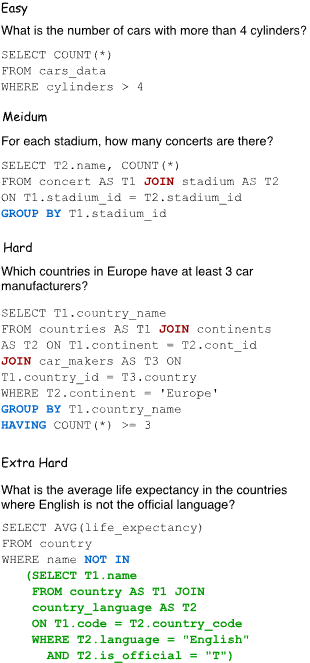
\includegraphics[width=0.35\textwidth]{image.png}
\caption{SQL query examples in 4 hardness levels. Credit: Spider (Yu et al., 2018)}
\label{fig:hardness-levels}
\end{figure}

\subsection{Prompting and Input}
\label{sec:prompting}

Each model receives three pieces of information in a single zero-shot user turn: a system instruction explaining its role as a Text-to-SQL generator, the database schema (Table names, column names, primary keys, and foreign-key relationships, with no example rows), and the natural-language question. No few-shot examples are provided, so that the experiment measures each model's ability to generate SQL from instructions and schema information alone, without the confound of examples steering its output style. The prompt template is identical across all three models, so that differences in performance can be attributed to the models rather than to differences in prompting.

\textbf{Prompt template:}
\begin{verbatim}
Given the following SQLite database schema, write a SQL query that answers
the question.

{schema}

Question: {question}

Respond with only the SQL query in a ```sql code block.
\end{verbatim}

See \hyperref[sec:appendix1]{Appendix 1} for a worked example: a full schema, a question, and the resulting filled prompt.

\subsection{SQL Extraction}
\label{sec:sql-extraction}

For each sample, we decode the model's generated tokens into text using the model-specific tokenizer, and check for the presence of a \texttt{</think>} token. If \texttt{</think>} was generated, we take all text generated before \texttt{</think>} as the reasoning trace and all text to the right as the output SQL; DeepSeek-R1-Distill-Qwen-1.5B is the only model of the three that can emit this token. The SQL is then extracted from the first \texttt{```sql} code block in that remaining text. The extracted SQL is passed to the evaluation script as-is. Outputs that cannot be extracted or parsed are counted as incorrect on every metric rather than excluded from the evaluation, as unusable output is a task failure (see \ref{sec:evaluation-metrics} and \ref{sec:invalid-outputs}).

\subsection{Inference Settings}
\label{sec:inference-settings}

All models are evaluated using the same decoding configuration: greedy decoding (temperature and top-p are not applicable) for consistent, reproducible results between runs. The maximum output length differs by model: 256 tokens for Qwen3-0.6B, and 4096 tokens for both Qwen3-4B and DeepSeek-R1-Distill-Qwen-1.5B. For DeepSeek, the larger budget is needed because its output also has to contain a full reasoning trace rather than only the SQL query; Qwen3-4B is given the same, larger budget as DeepSeek so that a tighter token limit can be ruled out as the reason for any difference between them on invalid-output rate (\ref{sec:invalid-outputs}) or inference time (\ref{sec:efficiency}). Qwen3-0.6B and Qwen3-4B are both run with thinking mode off (both support it). DeepSeek-R1-Distill-Qwen-1.5B always produces a reasoning trace and has no documented way to disable thinking mode, so it is evaluated as the reasoning condition against the two non-reasoning Qwen3 models. All inference runs on the same 1x RTX 4090 GPU described in \ref{sec:models}, with batch size 128.

\subsection{Evaluation}
\label{sec:evaluation-metrics}

We evaluate the output using the same metrics as the Spider paper (Yu et al., 2018). These are:

\begin{enumerate}
\item Component Matching
    \begin{itemize}
        \item For each of the following components:
        \begin{itemize}
            \item SELECT
            \item WHERE
            \item GROUP BY
            \item ORDER BY
            \item KEYWORDS (including all SQL keywords without column names and operators)
        \end{itemize}
        \item Decompose each component in the prediction and ground truth as bags of several sub-components and check whether or not these two sets of components match completely.
        \item Checks accuracy, recall, and F1
    \end{itemize}
\item Exact Matching Accuracy
    \begin{itemize}
        \item We measure whether the generated query as a whole is equivalent to the golden query (AKA ground truth query)
        \item The generated query is correct only if all components are correct
        \item Checks only accuracy
    \end{itemize}
\item Execution Accuracy
    \begin{itemize}
        \item A list of gold values for each question is given
        \item We measure how many gold values the generated query extracts when executed
        \item Checks only accuracy
    \end{itemize}
\end{enumerate}

If output is invalid or unparsable, then it fails exact matching and execution accuracy. Results~\ref{sec:invalid-outputs} reports how often this happens for each model.

\section{RQ1: Results}
\label{sec:rq1-results}

\subsection{Overall Model Performance}
\label{sec:overall-performance}

Below we report how Qwen3-0.6B, Qwen3-4B, and DeepSeek-R1-Distill-Qwen-1.5B perform on the Spider benchmark across all 3 metrics (Component Matching, Exact Matching Accuracy, Execution Accuracy). We calculate the values per problem difficulty as well as overall, and display them in the below tables.

\begin{table}[H]
\centering
\footnotesize
\caption{Overall performance summary, aggregated across all difficulties (all 1034 problems). Component matching is accuracy / recall / F1 (macro-averaged, see the note on Table~\ref{tab:difficulty-component} in \ref{sec:rq1-interpretation}). Per-difficulty breakdowns are in Tables~\ref{tab:difficulty-component}--\ref{tab:difficulty-execution}.}
\label{tab:overall-performance}
\resizebox{\textwidth}{!}{%
\begin{tabular}{lllccc}
\toprule
Model & Parameters & Category & Component matching & Exact matching & Execution accuracy \\
\midrule
Qwen3-0.6B & 0.6B & Decoder-only & 0.628 / 0.209 / 0.314 & 0.099 & 0.209 \\
Qwen3-4B & 4B & Decoder-only & 0.797 / 0.306 / 0.442 & 0.256 & 0.353 \\
DeepSeek-R1-Distill-Qwen-1.5B & 1.5B & Reasoning & 0.661 / 0.174 / 0.275 & 0.085 & 0.121 \\
\bottomrule
\end{tabular}}
\end{table}

All models are evaluated zero-shot with the same prompt on the 20 databases of the Spider dev set. Aggregated across all difficulties and databases, every model is still far from solving the task: execution accuracy ranges from 0.121 (DeepSeek) to 0.353 (Qwen3-4B) and exact matching accuracy from 0.085 (DeepSeek) to 0.256 (Qwen3-4B). Execution accuracy is higher than exact matching accuracy for all three models (for example 0.353 vs.\ 0.256 for Qwen3-4B), which suggests that at least some of the queries that return the correct result are written differently from the gold SQL (see Section \ref{sec:rq1-interpretation} for more on this relationship). Of the three models, Qwen3-4B is now the best on almost every metric, database, and difficulty level; Section \ref{sec:by-database} and Section \ref{sec:rq1-interpretation} quantify how consistently. Table ~\ref{tab:inference-time} reports the efficiency side of this comparison: inference time per example.

\subsection{Performance by Query Difficulty}
\label{sec:by-difficulty}

\begin{table}[H]
\centering
\footnotesize
\caption{Component matching (accuracy / recall / F1) by difficulty.}
\label{tab:difficulty-component}
\begin{tabular}{lcc}
\toprule
Model & easy & medium \\
\midrule
Problems (n) & 248 & 446 \\
Qwen3-0.6B & 0.675 / 0.308 / 0.423 & 0.582 / 0.235 / 0.334 \\
Qwen3-4B & 0.838 / 0.574 / 0.681 & 0.670 / 0.306 / 0.420 \\
DeepSeek-R1-Distill-Qwen-1.5B & 0.566 / 0.288 / 0.382 & 0.642 / 0.185 / 0.287 \\
\bottomrule
\end{tabular}

\vspace{0.5em}

\begin{tabular}{lccc}
\toprule
Model & hard & extra & all \\
\midrule
Problems (n) & 174 & 166 & 1034 \\
Qwen3-0.6B & 0.540 / 0.141 / 0.223 & 0.578 / 0.160 / 0.250 & 0.628 / 0.209 / 0.314 \\
Qwen3-4B & 0.796 / 0.262 / 0.394 & 0.485 / 0.150 / 0.229 & 0.797 / 0.306 / 0.442 \\
DeepSeek-R1-Distill-Qwen-1.5B & 0.543 / 0.113 / 0.187 & 0.389 / 0.104 / 0.164 & 0.661 / 0.174 / 0.275 \\
\bottomrule
\end{tabular}
\end{table}

\begin{table}[H]
\centering
\footnotesize
\caption{Exact matching accuracy by difficulty.}
\label{tab:difficulty-exact}
\begin{tabular}{lccccc}
\toprule
Model & easy & medium & hard & extra & all \\
\midrule
Problems (n) & 248 & 446 & 174 & 166 & 1034 \\
Qwen3-0.6B & 0.157 & 0.137 & 0.006 & 0.006 & 0.099 \\
Qwen3-4B & 0.508 & 0.262 & 0.115 & 0.012 & 0.256 \\
DeepSeek-R1-Distill-Qwen-1.5B & 0.214 & 0.078 & 0.000 & 0.000 & 0.085 \\
\bottomrule
\end{tabular}
\end{table}

\begin{table}[H]
\centering
\footnotesize
\caption{Execution accuracy by difficulty.}
\label{tab:difficulty-execution}
\begin{tabular}{lccccc}
\toprule
Model & easy & medium & hard & extra & all \\
\midrule
Problems (n) & 248 & 446 & 174 & 166 & 1034 \\
Qwen3-0.6B & 0.210 & 0.276 & 0.126 & 0.114 & 0.209 \\
Qwen3-4B & 0.565 & 0.345 & 0.276 & 0.139 & 0.353 \\
DeepSeek-R1-Distill-Qwen-1.5B & 0.258 & 0.128 & 0.017 & 0.006 & 0.121 \\
\bottomrule
\end{tabular}
\end{table}

We break every metric down by the Spider Hardness Criteria (\ref{sec:eval-data}), since aggregate numbers alone would hide whether a model's advantage holds up as queries get harder.

Performance decreases with difficulty for every model, but the decrease is steepest for Qwen3-0.6B and DeepSeek: their exact matching and execution accuracy are both at most 0.006 and 0.126 respectively on hard and extra problems, down from as high as 0.210-0.258 (easy execution) on the easiest problems (Table~\ref{tab:difficulty-exact} and Table~\ref{tab:difficulty-execution}). Qwen3-4B degrades on the same relative scale but from a much higher starting point, from 0.508 easy exact matching / 0.565 easy execution accuracy down to 0.012 extra exact matching / 0.139 extra execution accuracy. Despite the degradation, it remains the best of the three models at every single difficulty level on both metrics (Tables~\ref{tab:difficulty-exact}--\ref{tab:difficulty-execution}).

\subsection{Performance by Database}
\label{sec:by-database}

We also break execution and exact matching accuracy down by each of the 20 Spider dev databases. Qwen3-4B has the highest execution accuracy on 17 of the 20 databases outright (plus a tie on one more) and the highest exact matching accuracy on 18 of 20, while DeepSeek-R1-Distill-Qwen-1.5B is never highest on either metric; Qwen3-0.6B wins outright only on orchestra and battle\_death. Databases with few problems (real\_estate\_properties with n=4, voter\_1 with n=15, battle\_death with n=16, and museum\_visit with n=18) are too small to rank the models reliably, since a single problem changes a score by 6 to 25 percentage points. Execution accuracy ranges from 0.10 (course\_teach) to 0.53 (singer) for Qwen3-0.6B, from 0.19 (battle\_death) to 0.60 (singer) for Qwen3-4B, and from 0.00 (concert\_singer) to 0.27 (singer and voter\_1) for DeepSeek-R1-Distill-Qwen-1.5B (\hyperref[tab:db-execution]{Table 5}). 


\begin{table}[H]
\centering
\footnotesize
\caption{Execution accuracy by database (domain).}
\begin{tabular}{lcccc}
\toprule
Database & Problems (n) & Qwen3-0.6B & Qwen3-4B & DeepSeek-R1-Distill-Qwen-1.5B \\
\midrule
world\_1 & 120 & 0.183 & 0.242 & 0.108 \\
car\_1 & 92 & 0.109 & 0.315 & 0.054 \\
cre\_Doc\_Template\_Mgt & 84 & 0.202 & 0.405 & 0.071 \\
dog\_kennels & 82 & 0.159 & 0.293 & 0.085 \\
flight\_2 & 80 & 0.263 & 0.500 & 0.250 \\
student\_transcripts\_tracking & 78 & 0.128 & 0.321 & 0.064 \\
wta\_1 & 62 & 0.161 & 0.290 & 0.129 \\
tvshow & 62 & 0.339 & 0.435 & 0.129 \\
network\_1 & 56 & 0.286 & 0.375 & 0.179 \\
concert\_singer & 45 & 0.111 & 0.289 & 0.000 \\
pets\_1 & 42 & 0.167 & 0.286 & 0.071 \\
poker\_player & 40 & 0.250 & 0.550 & 0.225 \\
orchestra & 40 & 0.350 & 0.250 & 0.100 \\
employee\_hire\_evaluation & 38 & 0.105 & 0.211 & 0.132 \\
course\_teach & 30 & 0.100 & 0.500 & 0.100 \\
singer & 30 & 0.533 & 0.600 & 0.267 \\
museum\_visit & 18 & 0.278 & 0.500 & 0.222 \\
battle\_death & 16 & 0.375 & 0.188 & 0.188 \\
voter\_1 & 15 & 0.267 & 0.400 & 0.267 \\
real\_estate\_properties & 4 & 0.500 & 0.500 & 0.000 \\
\bottomrule
\label{tab:exec-acc-rq1-by-database}
\end{tabular}
\end{table}


The pattern on exact matching accuracy is just as one-sided (\hyperref[tab:db-exact]{Table 6}): Qwen3-4B is highest on 18 of 20 databases, ties Qwen3-0.6B on orchestra, and loses only on battle\_death; DeepSeek's exact matching accuracy is never the highest of the three, coming closest on flight\_2 (0.200 vs.\ Qwen3-4B's 0.350 and Qwen3-0.6B's 0.075). The full per-database tables and discussion are in \hyperref[sec:appendix2]{Appendix 2}.

\subsection{Analysis of Invalid and Unparseable Outputs}
\label{sec:invalid-outputs}

We also count how often each model's output cannot be used as SQL at all: it either never produces a usable query within the token budget (\ref{sec:inference-settings}) or is truncated before finishing one. Per \ref{sec:evaluation-metrics}, these count as failures on every metric rather than being excluded, and this is a direct measure of how reliably each model follows the ``respond with only a SQL query'' instruction, independent of whether the SQL it does produce is correct. Qwen3-0.6B's invalid rate is 2.2\%, Qwen3-4B's is 0.0\%, and DeepSeek-R1-Distill-Qwen-1.5B's is 9.7\%, about 4x higher than Qwen3-0.6B's despite having the same 4096-token budget as Qwen3-4B (\ref{sec:inference-settings}), i.e. a larger token budget did not cause Qwen3-4B to run on or produce unusable output the way it does for DeepSeek. Section \ref{sec:rq1-interpretation} breaks DeepSeek's failures down further by difficulty and by why the generation failed (see Tables~\ref{tab:deepseek-outcome}--\ref{tab:deepseek-unfinished-by-difficulty}).


\begin{table}[H]
\centering
\footnotesize
\caption{DeepSeek-R1-Distill-Qwen-1.5B by generation outcome. ``Cut'' means the generation reached the 4096-token limit.}
\label{tab:deepseek-outcome}
\begin{tabular}{lccccc}
\toprule
Outcome & Problems (n) & Share & Avg.\ tokens & Exact match & Component F1 \\
\midrule
Finished with SQL & 934 & 90.3\% & 512 & 0.094 & 0.286 \\
Finished, no usable SQL & 2 & 0.2\% & 284 & 0.000 & 0.100 \\
Cut while answering (after \texttt{</think>}) & 13 & 1.3\% & 4096 & 0.000 & 0.096 \\
Cut while thinking (no \texttt{</think>}) & 85 & 8.2\% & 4096 & 0.000 & 0.093 \\
All & 1034 & 100\% & 851 & 0.085 & 0.275 \\
\bottomrule
\end{tabular}
\end{table}

\begin{table}[H]
\centering
\footnotesize
\caption{The same 934 questions that DeepSeek finished, for all three models.}
\label{tab:deepseek-finished-934}
\begin{tabular}{lcc}
\toprule
Model & Exact match & Component F1 \\
\midrule
DeepSeek-R1-Distill-Qwen-1.5B & 0.094 & 0.286 \\
Qwen3-0.6B & 0.103 & 0.317 \\
Qwen3-4B & 0.257 & 0.440 \\
\bottomrule
\end{tabular}
\end{table}

\begin{table}[H]
\centering
\footnotesize
\caption{Share of Deepseek generations that are infinite self-repetition loops. We check self-repetition using compression ratio: a text that repeats itself compresses well, so a low compression ratio of the last 3000 characters indicates a loop. In testing, we found generations with compression ratios <0.15 infinitely self-looped.}
\label{tab:deepseek-repetition}
\begin{tabular}{lcccc}
\toprule
Generations & n & Median compression ratio & Ratio $<$ 0.15 & Last 150 characters repeat 3 or more times \\
\midrule
Cut off & 98 & 0.095 & 95.9\% & 96.9\% \\
Finished & 936 & 0.418 & 0.0\% & 0.2\% \\
\bottomrule
\end{tabular}
\end{table}

\begin{table}[H]
\centering
\footnotesize
\caption{Share of DeepSeek generations that did not finish with SQL, by difficulty.}
\label{tab:deepseek-unfinished-by-difficulty}
\begin{tabular}{lccccc}
\toprule
 & easy & medium & hard & extra & all \\
\midrule
Problems (n) & 248 & 446 & 174 & 166 & 1034 \\
Not finished with SQL (n) & 15 & 33 & 25 & 27 & 100 \\
Share & 6.0\% & 7.4\% & 14.4\% & 16.3\% & 9.7\% \\
\bottomrule
\end{tabular}
\end{table}

\subsection{Efficiency Measures}
\label{sec:efficiency}

\begin{table}[H]
\centering
\footnotesize
\caption{Output tokens per example.}
\label{tab:tokens-per-example}
\begin{tabular}{lccccc}
\toprule
Model & easy & medium & hard & extra & all \\
\midrule
Qwen3-0.6B & 27.5 & 44.7 & 53.7 & 69.9 & 46.1 \\
Qwen3-4B & 23.6 & 37.3 & 46.2 & 59.0 & 39.0 \\
DeepSeek-R1-Distill-Qwen-1.5B & 610.8 & 768.4 & 1096.0 & 1176.9 & 851.3 \\
\bottomrule
\end{tabular}
\end{table}

Inference time is measured from the start of generation to the complete batch output, per batch of 128 examples, with each batch's wall time divided evenly across its 128 examples to get the per-example figure, excluding tokenization, model loading, and warm-up.

\begin{table}[H]
\centering
\footnotesize
\caption{Inference time.}
\label{tab:inference-time}
\begin{tabular}{lcc}
\toprule
Model & Total wall time (s) & Avg.\ time per example (s) \\
\midrule
Qwen3-0.6B & 123.9 & 0.120 \\
Qwen3-4B & 109.1 & 0.106 \\
DeepSeek-R1-Distill-Qwen-1.5B & 3059.8 & 2.959 \\
\bottomrule
\end{tabular}
\end{table}

DeepSeek is about 25x slower per example than Qwen3-0.6B and 28x slower than Qwen3-4B, consistent with its much higher average token count (Table~\ref{tab:tokens-per-example}). Qwen3-4B, despite having about 7x as many parameters as Qwen3-0.6B, is marginally faster per example (0.106s vs.\ 0.120s), consistent with it generating fewer tokens on average (39.0 vs.\ 46.1, Table~\ref{tab:tokens-per-example}) despite having the same 16x larger token budget as DeepSeek (\ref{sec:inference-settings}).


\section{RQ1: Interpretation and Answer}
\label{sec:rq1-interpretation}

\textbf{RQ1:} How do (selected) LLMs perform on cross-domain Text-to-SQL?

\vspace{10px}

All three models are still far from solving the task in this zero-shot setting: exact matching accuracy ranges from 0.085 to 0.256 and execution accuracy from 0.121 to 0.353 (Table~\ref{tab:overall-performance}). Difficulty and database effects are discussed in \ref{sec:by-difficulty} and \ref{sec:by-database}; here we interpret the effects of model size and reasoning architecture and the exact-match/execution-accuracy relationship, and state the answer to RQ1 as three findings.

\subsection{First, within the Qwen family, scale is a strong and almost uniform predictor of performance, but an intermediate-size reasoning model from the DeepSeek family still loses to the smallest model in the Qwen family.}
\label{sec:rq1-finding-scale}

Aggregated across all difficulties, Qwen3-4B has the best component matching (0.797 accuracy / 0.306 recall / 0.442 F1), exact matching (0.256 ), and execution accuracy (0.353) of the three (Table~\ref{tab:overall-performance}), and it beats Qwen3-0.6B on exact matching and execution accuracy at every individual difficulty level, including hard (0.115 vs.\ 0.006) and extra (0.012 vs.\ 0.006), where the smaller model solves almost nothing (Tables~\ref{tab:difficulty-exact}--\ref{tab:difficulty-execution}). This effect is large and holds at every difficulty level. The one exception is component matching on extra-hard problems, where Qwen3-0.6B's accuracy, recall, and F1 (0.578 / 0.160 / 0.250) are all slightly higher than Qwen3-4B's (0.485 / 0.150 / 0.229), the only point in the RQ1 results where the smaller Qwen3 model wins outright (Table~\ref{tab:difficulty-component}). DeepSeek-R1-Distill-Qwen-1.5B sits between the two Qwen3 models in parameter count (1.5B) and is the only one that reasons, yet it is the lowest of the three on every aggregate metric (0.275 component F1, 0.085 exact matching, 0.121 execution accuracy) except its own component-matching accuracy (0.661 vs.\ 0.628 for Qwen3-0.6B). Thus, scale predicts performance well within a family, but does not transfer across the reasoning/non-reasoning boundary: having more parameters than Qwen3-0.6B did not help DeepSeek catch up to it.

\subsection{Second, the reasoning architecture itself, not parameter count, is the most likely driver of DeepSeek's low score.}
\label{sec:rq1-finding-reasoning}

Its invalid-output rate (9.7\%) is markedly higher than Qwen3-0.6B's (2.2\%) and Qwen3-4B's (0.0\% in this run) (\ref{sec:invalid-outputs}). In Tables~\ref{tab:deepseek-outcome}--\ref{tab:deepseek-unfinished-by-difficulty}, 100 of 1034 generations (9.7\%) end without usable SQL. 85 never leave the reasoning phase, 13 are cut while writing the answer, and 2 finish without SQL. The number of unusable SQL generations also grows with difficulty, from 6.0\% on easy to 16.3\% on extra problems. These are not cases of long productive reasoning either: 95.9\% of the cut-off generations are highly self-repetitive (compression ratio below 0.15, median compression ratio 0.095, vs.\ 0.418 for finished generations), rewriting the same query and repeating phrases like ``So the final query is:'' without converging. Finishing does not make it better either: on the 934 questions DeepSeek does finish, its exact matching (0.094) and component F1 (0.286) are still below Qwen3-0.6B's on the same questions (0.103 / 0.317) and far below Qwen3-4B's (0.257 / 0.440), despite generating 512 tokens per question on average there, against 46 and 39 tokens overall for Qwen3-0.6B and Qwen3-4B (about 11x and 13x fewer). This extra length also costs time: DeepSeek is 25-28x slower per example than either Qwen3 model (\ref{sec:efficiency}). The reasoning trace mostly lengthens the output and sometimes never terminates, without improving the SQL when it does, and size alone is not the explanation, since Qwen3-4B is both bigger than DeepSeek and the best model in the comparison. This does not fully isolate reasoning from DeepSeek's other differences from the two Qwen3 models, such as distillation (see Limitations).

\subsection{Third, query difficulty has a substantial, consistent effect on every model, including the best one.}
\label{sec:rq1-finding-difficulty}

Exact matching and execution accuracy both fall sharply from easy to extra-hard problems for all three models (\ref{sec:by-difficulty}). Qwen3-4B's drop is from a much higher base (0.508 to 0.012 exact matching, 0.565 to 0.139 execution accuracy) and it remains the best model at every difficulty level on both metrics, but the drop itself is just as steep in relative terms as for the other two models, and the hardest problems remain largely unsolved even for it.

\subsection{Exact Match vs.\ Execution Accuracy}
\label{sec:rq1-exact-vs-execution}

For all three models, execution accuracy aggregated across all difficulties exceeds exact matching accuracy (Table~\ref{tab:overall-performance}): 0.209 vs.\ 0.099 for Qwen3-0.6B, 0.353 vs.\ 0.256 for Qwen3-4B, and 0.121 vs.\ 0.085 for DeepSeek. Since exact matching requires every SQL component to match the gold query while execution accuracy only requires the same result set, this gap indicates each model writes some queries that are valid and correct but phrased differently from the gold SQL (e.g.\ a different but equivalent join order, or an explicit column list where the gold query uses \texttt{SELECT *}). The gap is widest for Qwen3-0.6B (11.0 points), close behind for Qwen3-4B (9.7 points), and narrowest for DeepSeek (3.6 points); DeepSeek's narrower gap reflects it producing fewer alternative-but-valid queries. Qwen3-4B's gap is almost as wide as Qwen3-0.6B's despite much higher absolute accuracy, so scaling up within the Qwen3 family raises both exact matching accuracy and execution accuracy together rather than closing the gap between them.

\subsection{Limitations}
\label{sec:rq1-limitations}

Our working hypothesis is that Text-to-SQL at this scale does not benefit from an explicit reasoning trace, and that a non-reasoning model is sufficient, with performance instead scaling with parameter count within a fixed model family. The results are consistent with this hypothesis. However, they do not establish that Text-to-SQL is too simple for reasoning models in general due to several factors:

\begin{itemize}
\item \textbf{Model differences beyond reasoning.} Qwen3-0.6B and Qwen3-4B share a model family, isolating the effect of scale between them, but DeepSeek differs from both in family, size, and pretraining/post-training, not only in whether it reasons; it is also a distilled model, so the effect of reasoning cannot be fully separated from distillation quality.
\item \textbf{Aggregated component matching.} The component matching figures in Table~\ref{tab:difficulty-component} (and in Table~\ref{tab:overall-performance}) are our own macro-average (mean of the 10 per-component accuracy and recall scores, with F1 computed from these two means), not a number reported by Spider.
\end{itemize}

Overall, in this zero-shot, cross-domain setting, a larger non-reasoning decoder-only model (Qwen3-4B, 4B) clearly outperforms both a same-family model at under a sixth its size (Qwen3-0.6B) and a reasoning model of intermediate size from a different family (DeepSeek-R1-Distill-Qwen-1.5B, 1.5B), while also being faster per example than either. None of the three models solve more than half of even the easiest problems or more than a small fraction of hard or extra-hard queries. This answers RQ1 for the three models evaluated.
% RQ2.tex -- Task 2 / RQ2 section, part of the report/ directory (see main.tex).
%
% Intended use: % RQ2.tex -- Task 2 / RQ2 section, part of the report/ directory (see main.tex).
%
% Intended use: % RQ2.tex -- Task 2 / RQ2 section, part of the report/ directory (see main.tex).
%
% Intended use: \input{RQ2} into main.tex, after \input{RQ1} (this
% file's cross-references into Task 1 -- table~\ref{tab:deepseek-outcome},
% \ref{tab:tokens-per-example}, \ref{sec:sql-extraction}, etc. -- rely on
% RQ1.tex's labels already being defined earlier in the same document).
%
% Structure: Methodology is organized per-feature (Feature 1: Token Count,
% Feature 2: Information Retention), each with its own Definition / Why it's
% relevant / How we computed it. Results is organized as descriptive
% statistics, differences by correctness, differences by difficulty, and
% relationship with Text-to-SQL correctness (the correlation analysis).

\section{Task 2 -- RQ2: Methodology}
\label{sec:rq2-methodology}

\textbf{RQ2:} How do characteristics of reasoning traces (of reasoning LLM) relate to Text-to-SQL performance?

To answer this question, we examine two features of each reasoning trace: Token Count and Information Retention. We compute both for all 1034 generations in DeepSeek-R1-Distill-Qwen-1.5B's main Task 1 run, then relate each to difficulty and to Text-to-SQL correctness.

\subsection{Feature 1: Token Count}
\label{sec:rq2-feature-tokencount}

\textbf{Definition.} Token Count is the number of tokens in the reasoning segment of a generation, i.e.\ everything the model generates before \texttt{</think>}, excluding the final SQL answer. We split each generation into a reasoning segment and an answer segment using the same \texttt{</think>} split used in Task 1 (\ref{sec:sql-extraction}).

% We hypothesize that for each difficulty there exists a "goldilocks" token-count range, and that performance improves as the answer's token count approaches the mean of that range.

\textbf{Why it's relevant.} Examining token count allows us to investigate whether the amount of generated reasoning is associated with better Text-to-SQL performance. However, a longer trace does not necessarily mean better reasoning, since additional tokens may contain redundant or irrelevant information.

Additionally, we expect Token Count to scale positively with the difficulty of the related Text-to-SQL problem: easy questions should require fewer thinking tokens, while extra-hard questions should require significantly more. Any question that disobeys this relation, or where more tokens associate with worse rather than better answers, is given special attention in Results.

\textbf{How we computed it.} Token Count is the number of tokens in the reasoning segment only, re-tokenized with the model's own tokenizer (not the \texttt{new\_tokens} field logged during generation, which counts the whole generation, reasoning plus SQL). For generations that never emit \texttt{</think>} (truncated at the 4096-token generation limit, see Task 1's table~\ref{tab:deepseek-outcome}), the entire generated text is treated as the reasoning segment, so Token Count for these rows is effectively capped at the generation limit rather than reflecting a completed thought. This is intentional: these cases are exactly the repetition loops Task 1 identified (table~\ref{tab:deepseek-repetition}), and dropping them would hide, rather than explain, the heavy right tail in Token Count. We keep them in the Token Count analysis and flag wherever they drive a result (see finding~\ref{item:rq2-finding-tokencount-difficulty} in Results).

\begin{table}[H]
\centering
\footnotesize
\caption{Token Count: definition and computation summary.}
\label{tab:rq2-feature-tokencount-summary}
\begin{tabular}{p{0.22\textwidth}p{0.7\textwidth}}
\toprule
Property & Detail \\
\midrule
Unit & Tokens (model's own tokenizer) \\
Scope & Reasoning segment only, i.e.\ text before \texttt{</think>} \\
Range & Non-negative integer, long right tail (observed 103--4166) \\
Truncated traces & Treated as reasoning segment in full; capped at the 4096-token generation limit \\
\bottomrule
\end{tabular}
\end{table}

\subsection{Feature 2: Information Retention}
\label{sec:rq2-feature-retention}

\textbf{Definition.} Information Retention is the share of schema-shaped identifiers mentioned in a reasoning trace that actually exist as a table or column name in that question's schema. Equivalently, $$(1-\text{Information Retention})=\text{fraction of mentioned identifiers that are not grounded in the prompt}$$ or in other words, the hallucination rate of the trace.

\textbf{Why it's relevant.} We expect reasoning traces with low Information Retention (frequent hallucination of schema elements) to produce lower-performing answers than traces that stay grounded in the given schema, since inventing a table or column that doesn't exist is very likely to propagate into an incorrect query. We also expect harder problems to not cause lower Information Retention on their own; if they do, this points to the model introducing more assumptions as questions get harder, which is itself worth investigating as a bias rather than attributing the accuracy drop to difficulty alone.

\textbf{How we computed it.} We regex-extract every schema-shaped identifier the trace mentions, either quoted (e.g.\ \texttt{"Singer\_ID"}) or underscore-joined (e.g.\ \texttt{concert\_id}), and take the share of those identifiers that match a table or column name in that question's schema. An identifier that matches neither is treated as a fact the model introduced on its own, i.e., a hallucination. Traces that mention no schema identifiers at all are excluded from Information Retention (but kept for Token Count), since a 0-of-0 ratio is undefined rather than evidence of perfect or zero retention; this drops the usable sample from 1034 to 1017.

\begin{table}[H]
\centering
\footnotesize
\caption{Information Retention: definition and computation summary.}
\label{tab:rq2-feature-retention-summary}
\begin{tabular}{p{0.22\textwidth}p{0.7\textwidth}}
\toprule
Property & Detail \\
\midrule
Unit & Ratio, bounded in $[0,1]$ \\
Numerator & Schema identifiers mentioned in the trace that match a real table/column name \\
Denominator & All schema-shaped identifiers mentioned in the trace (quoted or underscore-joined) \\
Exclusions & Traces mentioning zero schema identifiers (1034 $\rightarrow$ 1017 usable rows) \\
Truncated traces & Scored over the partial text generated before truncation \\
\bottomrule
\end{tabular}
\end{table}

\subsection{Statistical approach}
\label{sec:rq2-statistical-approach}

We relate both Token Count and Information Retention to correctness and difficulty with Spearman's Rank Correlation throughout. Both of our hypotheses are about monotonic relationships, not linear relationships (performance should not decrease as Token Count or Information Retention increase, and Token Count should increase with difficulty), which is exactly what Spearman's Rank Correlation tests for. It also suits the distribution of our two reasoning metrics: Token Count is a non-negative count with a long right tail (DeepSeek alone ranges from 611 tokens on easy problems to 1177 on extra, table~\ref{tab:tokens-per-example}), and Information Retention is a bounded ratio, so neither is likely to be symmetric and unbounded; the $\geq$90\% trace completion rate gives us enough data per stratum to check this on histograms rather than assume it. For correctness, we correlate each reasoning metric against the continuous, per-question component matching accuracy, recall, and F1 for all ten Spider components individually, plus exact matching and execution accuracy.

This gives 32 submetrics per reasoning metric per difficulty level. With 169 correlation tests run in total, we correct for multiple comparisons with the Benjamini-Hochberg procedure rather than a stricter family-wise correction like Bonferroni: we are screening many related, non-independent submetrics for the strongest associations to report and discuss, not making a small number of pre-registered confirmatory claims, so controlling the expected false-discovery rate is a better fit than controlling the probability of any single false positive at the cost of statistical power.

% The Results below report Token Count and Information Retention broken down two ways: by difficulty, since that is the primary hypothesis under test, and by exact-match correctness (correct/incorrect), used for the descriptive statistics and the boxplots (figure~\ref{fig:rq2-boxplots}) because a binary split is easier to read in a table or figure than 32 continuous submetrics. The correlation analysis itself (table~\ref{tab:rq2-correlations}) still uses the continuous submetrics described above, for the statistical-power reasons given there; the binary-correctness view and the continuous-submetric view are two presentations of the same underlying data, not two different analyses.

The Results below report Token Count and Information Retention by correctness and difficulty level, with the continuous submetrics used directly in the correlation analysis (Table~\ref{tab:rq2-correlations}).


\section{RQ2: Results}
\label{sec:rq2-results}

We compute Token Count and Information Retention for all 1034 generations in DeepSeek-R1-Distill-Qwen-1.5B's main Task 1 run, and correlate each against difficulty and against all 32 per-question performance submetrics as described in the Methodology. Tables ~\ref{tab:rq2-descriptive-stats-tokencount-difficulty}, ~\ref{tab:rq2-descriptive-stats-tokencount-correctness}, ~\ref{tab:rq2-descriptive-stats-retention-difficulty}, and~\ref{tab:rq2-descriptive-stats-retention-correctness} give descriptive statistics for each feature by difficulty and by exact-match correctness; figure~\ref{fig:rq2-boxplots} shows the resulting distributions; table~\ref{tab:rq2-correlations} lists the strongest correlations.

\subsection{Descriptive statistics}
\label{sec:rq2-descriptive-stats}


\begin{table}[H]
\centering
\footnotesize
\caption{Token Count descriptive statistics, by difficulty.}
\label{tab:rq2-descriptive-stats-tokencount-difficulty}
\begin{tabular}{lcccccc}
\toprule
Group & n & mean & median & std & min & max \\
\midrule
easy & 248 & 542.3 & 329.0 & 845.2 & 103 & 4096 \\
medium & 446 & 648.2 & 374.0 & 925.7 & 191 & 4166 \\
hard & 174 & 939.2 & 425.0 & 1246.2 & 226 & 4096 \\
extra & 166 & 901.6 & 434.5 & 1199.9 & 222 & 4096 \\
\midrule
all & 1034 & 712.4 & 383.0 & 1026.2 & 103 & 4166 \\
\bottomrule
\end{tabular}
\end{table}

\begin{table}[H]
\centering
\footnotesize
\caption{Token Count descriptive statistics, by exact-match correctness (1 = exact match, 0 = not).}
\label{tab:rq2-descriptive-stats-tokencount-correctness}
\begin{tabular}{lcccccc}
\toprule
Group & n & mean & median & std & min & max \\
\midrule
exact match = 0 & 946 & 748.1 & 394.0 & 1065.6 & 103 & 4166 \\
exact match = 1 & 88 & 329.3 & 314.5 & 97.7 & 195 & 849 \\
\midrule
all & 1034 & 712.4 & 383.0 & 1026.2 & 103 & 4166 \\
\bottomrule
\end{tabular}
\end{table}

\begin{table}[H]
\centering
\footnotesize
\caption{Information Retention descriptive statistics, by difficulty. Excludes traces that mention no schema identifiers (n drops from 1034 to 1017 overall).}
\label{tab:rq2-descriptive-stats-retention-difficulty}
\begin{tabular}{lcccccc}
\toprule
Group & n & mean & median & std & min & max \\
\midrule
easy & 246 & 0.915 & 1.0 & 0.146 & 0.0 & 1.0 \\
medium & 441 & 0.905 & 1.0 & 0.148 & 0.0 & 1.0 \\
hard & 172 & 0.877 & 1.0 & 0.163 & 0.0 & 1.0 \\
extra & 158 & 0.861 & 1.0 & 0.215 & 0.0 & 1.0 \\
\midrule
all & 1017 & 0.896 & 1.0 & 0.163 & 0.0 & 1.0 \\
\bottomrule
\end{tabular}
\end{table}

\begin{table}[H]
\centering
\footnotesize
\caption{Information Retention descriptive statistics, by exact-match correctness (1 = exact match, 0 = not). Excludes traces that mention no schema identifiers (n drops from 1034 to 1017 overall).}
\label{tab:rq2-descriptive-stats-retention-correctness}
\begin{tabular}{lcccccc}
\toprule
Group & n & mean & median & std & min & max \\
\midrule
exact match = 0 & 931 & 0.893 & 1.0 & 0.166 & 0.0 & 1.0 \\
exact match = 1 & 86 & 0.924 & 1.0 & 0.123 & 0.5 & 1.0 \\
\midrule
all & 1017 & 0.896 & 1.0 & 0.163 & 0.0 & 1.0 \\
\bottomrule
\end{tabular}
\end{table}


\begin{figure}[H]
\centering
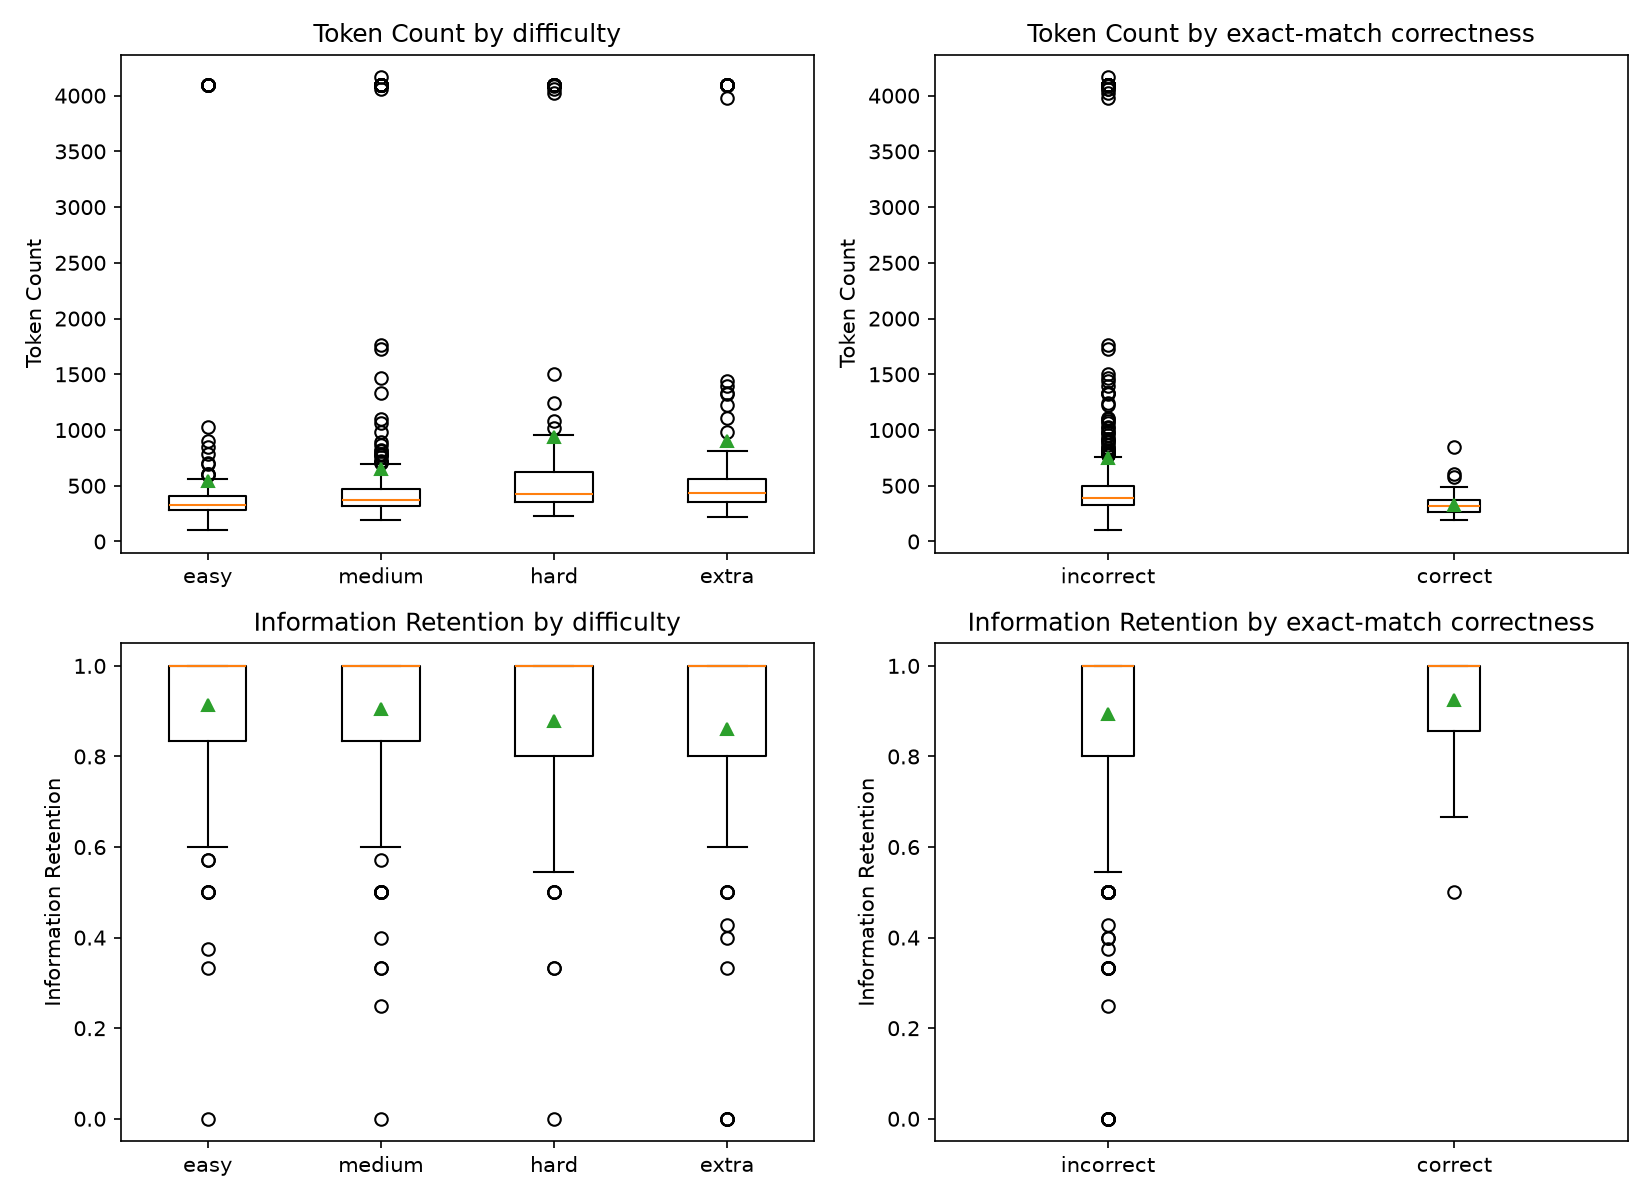
\includegraphics[width=0.85\textwidth]{boxplots.png}
\caption{Token Count and Information Retention by difficulty and by exact-match correctness, for DeepSeek-R1-Distill-Qwen-1.5B's 1034 Task 1 generations. Green triangles are means, orange lines are medians. Means sit well above medians throughout, confirming the right-skewed, bounded distributions the Methodology assumes rather than normal ones.}
\label{fig:rq2-boxplots}
\end{figure}

\subsection{Differences by correctness}
\label{sec:rq2-by-correctness}

Correct generations (exact match = 1) have a much lower mean and tighter spread of Token Count (329.3, std 97.7) than incorrect ones (748.1, std 1065.6, table~\ref{tab:rq2-descriptive-stats-tokencount-correctness}), and a slightly higher mean Information Retention (0.924 vs.\ 0.893, table~\ref{tab:rq2-descriptive-stats-retention-correctness}). Both differences point the same direction as the correlation findings in \ref{sec:rq2-relationship-correctness}: more reasoning tokens and lower retention associate with worse performance. The gap is far larger for Token Count than for Information Retention: incorrect generations' Token Count std (1065.6) is more than ten times that of correct generations (97.7), driven by the truncated, repetition-loop traces described in \ref{sec:rq2-feature-tokencount}, almost none of which are exact matches. Information Retention's median is 1.0 in both correctness groups, so the correctness gap in retention lives entirely in the mean and the lower tail, not in a shift of the typical trace. Overall, correctness tracks Token Count far more strongly than it tracks Information Retention, both in effect size and in where the gap shows up in the distribution.

\subsection{Differences by difficulty}
\label{sec:rq2-by-difficulty}

\begin{enumerate}
\item \label{item:rq2-finding-tokencount-difficulty} \textbf{Token Count increases with difficulty, as hypothesized, but the increase is driven by a heavy tail.} Median token count rises from 329 (easy) to 374 (medium) to 425 (hard) to 434 (extra), and the correlation with difficulty is positive and significant ($\rho=0.313$, $q<0.001$). The mean rises faster than the median at every level (for example 542 vs.\ 329 on easy), because generations hitting the 4096-token limit occur at every difficulty (figure~\ref{fig:rq2-boxplots}, top row); these are the same repetition loops Task 1 identified, not productive extra reasoning on harder problems.
\item \label{item:rq2-finding-retention-difficulty} \textbf{Information Retention decreases slightly with difficulty.} Median retention is 1.0 at every difficulty level, but the mean falls from 0.915 (easy) to 0.861 (extra), and the correlation with difficulty is negative and significant ($\rho=-0.107$, $q=0.013$). This is the case flagged in \ref{sec:rq2-feature-retention} as calling for closer examination of the model's introduced assumptions on harder problems.
\end{enumerate}

\subsection{Relationship with Text-to-SQL}
\label{sec:rq2-relationship-correctness}

\begin{enumerate}
\item \label{item:rq2-finding-tokencount-disobey} \textbf{On easy and medium problems, higher Token Counts track worse performance.} Token Count correlates negatively with \texttt{keywords} F1 on easy ($\rho=-0.42$, $q<0.001$) and medium ($\rho=-0.19$, $q<0.001$) problems, and with \texttt{where} and \texttt{where(no OP)} F1 on easy problems ($\rho=-0.32$ and $-0.33$, $q<0.001$). Knowing token count increases with difficulty (see ~\ref{sec:rq2-by-difficulty}), the extra tokens on these problems look like run-away generation rather than helpful deliberation.
\item \label{item:rq2-finding-retention-performance} \textbf{Where Information Retention relates to performance, it is mostly positive, as hypothesized.} On medium problems, Information Retention correlates positively with \texttt{where} and \texttt{where(no OP)} F1 ($\rho=0.345$, $q<0.001$ for both). Of its 82 submetric tests, 8 remain significant after Benjamini-Hochberg correction, 7 positive and 1 negative (\texttt{where(no OP)} recall on easy problems, $\rho=-0.261$, $q=0.042$).

\begin{table}[H]
\centering
\footnotesize
\caption{Strongest Spearman correlations between reasoning metrics and performance submetrics, Benjamini-Hochberg corrected, top 8 of 169 tests by q-value.}
\label{tab:rq2-correlations}
\begin{tabular}{llcccc}
\toprule
Metric & Submetric & Difficulty & n & $\rho$ & $q$ \\
\midrule
Token Count & difficulty (overall) & all & 1034 & 0.313 & $<$0.001 \\
Information Retention & \texttt{where} F1 & medium & 441 & 0.345 & $<$0.001 \\
Information Retention & \texttt{where(no OP)} F1 & medium & 441 & 0.345 & $<$0.001 \\
Token Count & \texttt{keywords} F1 & easy & 248 & -0.417 & $<$0.001 \\
Token Count & \texttt{where(no OP)} F1 & easy & 248 & -0.332 & $<$0.001 \\
Token Count & \texttt{where} F1 & easy & 248 & -0.322 & $<$0.001 \\
Token Count & \texttt{keywords} F1 & medium & 446 & -0.194 & $<$0.001 \\
Information Retention & difficulty (overall) & all & 1017 & -0.107 & 0.013 \\
\bottomrule
\end{tabular}
\end{table}

% \subsection{Verification: regression controlling for confounds}
% \label{sec:rq2-robustness}

% Sections~\ref{sec:rq2-by-difficulty} and~\ref{sec:rq2-relationship-correctness} test each feature against performance one at a time, but Token Count, Information Retention, and difficulty are not independent of one another: a bivariate finding there could really be driven by one of the other two variables rather than by the feature itself. The regressions below fit all three predictors jointly as statistical models, so each coefficient reflects that predictor's relationship with the outcome after the parts explained by the other two are removed, directly checking whether the findings above survive or are confounded.

% \begin{table}[H]
% \centering
% \footnotesize
% \caption{Logistic regression: exact match on standardized log Token Count, standardized Information Retention, and standardized difficulty, fit jointly ($n=1017$, pseudo $R^2=0.188$). OR is the odds ratio per one-SD increase in the predictor.}
% \label{tab:rq2-logistic}
% \begin{tabular}{lccccc}
% \toprule
% Predictor & coef & SE & $z$ & $p$ & OR [95\% CI] \\
% \midrule
% Intercept & -3.351 & 0.227 & -14.76 & $<$0.001 & 0.035 [0.022, 0.055] \\
% log Token Count ($z$) & -1.087 & 0.300 & -3.62 & $<$0.001 & 0.337 [0.187, 0.607] \\
% Information Retention ($z$) & 0.091 & 0.139 & 0.65 & 0.514 & 1.095 [0.834, 1.437] \\
% Difficulty ($z$) & -1.278 & 0.201 & -6.35 & $<$0.001 & 0.279 [0.188, 0.413] \\
% \bottomrule
% \end{tabular}
% \end{table}

% \begin{table}[H]
% \centering
% \footnotesize
% \caption{Proportional-odds (ordinal) regression: difficulty on standardized log Token Count and standardized Information Retention, fit jointly ($n=1017$). OR is the odds ratio per one-SD increase in the predictor.}
% \label{tab:rq2-ordinal}
% \begin{tabular}{lccccc}
% \toprule
% Predictor & coef & SE & $z$ & $p$ & OR [95\% CI] \\
% \midrule
% log Token Count ($z$) & 0.398 & 0.059 & 6.78 & $<$0.001 & 1.489 [1.327, 1.670] \\
% Information Retention ($z$) & -0.177 & 0.059 & -2.99 & 0.003 & 0.837 [0.746, 0.941] \\
% \bottomrule
% \end{tabular}
% \end{table}

% Controlling for the other feature and for difficulty changes which bivariate relationship survives. Token Count's association with correctness holds up: each one-SD increase in log Token Count is associated with 66\% lower odds of an exact match (OR$=0.337$, $p<0.001$), holding Information Retention and difficulty fixed (table~\ref{tab:rq2-logistic}) --- consistent with, and strengthening, finding~\ref{item:rq2-finding-tokencount-disobey}. Information Retention's association with correctness does not survive the same control (OR$=1.095$, $p=0.514$): once Token Count and difficulty are accounted for, Retention has no detectable independent effect on correctness, so the positive finding in \ref{item:rq2-finding-retention-performance} should be read as a submetric-specific, not a global, relationship. Both features' difficulty relationships, in contrast, are independent of one another: the ordinal regression finds Token Count still predicts higher difficulty (OR$=1.489$ per SD, $p<0.001$) and Information Retention still predicts lower difficulty (OR$=0.837$ per SD, $p=0.003$) when controlling for each other (table~\ref{tab:rq2-ordinal}), so neither difficulty trend in \ref{sec:rq2-by-difficulty} is simply a byproduct of the other feature's trend.

% \subsection{Regression diagnostics}
% \label{sec:rq2-diagnostics}

% The regressions in~\ref{sec:rq2-robustness} are only as trustworthy as their assumptions: if the three predictors are collinear, or if the ordinal model's proportional-odds assumption doesn't hold, the coefficients and significance levels reported there could be misleading rather than reflecting genuine independent effects. The checks below test both before those results are treated as confirmed.

% \begin{table}[H]
% \centering
% \footnotesize
% \caption{Variance inflation factors for the three predictors in the logistic regression (table~\ref{tab:rq2-logistic}).}
% \label{tab:rq2-vif}
% \begin{tabular}{lc}
% \toprule
% Predictor & VIF \\
% \midrule
% log Token Count ($z$) & 1.057 \\
% Information Retention ($z$) & 1.020 \\
% Difficulty ($z$) & 1.059 \\
% \bottomrule
% \end{tabular}
% \end{table}

% \begin{table}[H]
% \centering
% \footnotesize
% \caption{Proportional-odds check: the pooled ordinal-regression coefficient (table~\ref{tab:rq2-ordinal}) against three separately-fit cumulative-logit models, one per difficulty cutoff. Large, systematic drift across cutoffs would indicate the proportional-odds assumption does not hold.}
% \label{tab:rq2-po-check}
% \begin{tabular}{lcccc}
% \toprule
% Cutoff & coef (Token Count) & SE & coef (Retention) & SE \\
% \midrule
% pooled (proportional-odds) & 0.398 & 0.059 & -0.177 & 0.059 \\
% $P(\text{difficulty} \geq \text{medium})$ & 0.576 & 0.117 & -0.128 & 0.081 \\
% $P(\text{difficulty} \geq \text{hard})$ & 0.396 & 0.066 & -0.195 & 0.067 \\
% $P(\text{difficulty} \geq \text{extra})$ & 0.271 & 0.074 & -0.193 & 0.078 \\
% \bottomrule
% \end{tabular}
% \end{table}

% The three predictors in the logistic regression are not meaningfully collinear (all VIF $\approx 1.0$--$1.06$, well below the common rule-of-thumb threshold of 5, table~\ref{tab:rq2-vif}), so the coefficient estimates and significance levels reported in \ref{sec:rq2-robustness} are not an artifact of Token Count, Information Retention and difficulty standing in for one another. The proportional-odds check is more mixed. Information Retention's cumulative-logit coefficient is stable across all three cutoffs ($-0.128$, $-0.195$, $-0.193$, table~\ref{tab:rq2-po-check}), consistent with the pooled $-0.177$ and with the proportional-odds assumption holding for this feature. Token Count's coefficient, however, declines monotonically across cutoffs (0.576 at the easy/medium boundary, down to 0.271 at the hard/extra boundary): Token Count distinguishes difficulty levels well at the low end but loses discriminative power at the high end, a mild violation of the proportional-odds assumption that the single pooled coefficient in table~\ref{tab:rq2-ordinal} averages over. This does not overturn the ordinal regression's conclusion that Token Count predicts difficulty (every individual cutoff coefficient is still positive and more than 3 standard errors from zero), but it means the pooled OR$=1.489$ should be read as an average effect across difficulty levels rather than a uniform one.
 into main.tex, after \usepackage{upquote}

\section{Task 1 -- RQ1: Methodology \& Results}
\label{sec:rq1-methods}

\textbf{RQ1:} How do (selected) LLMs perform on cross-domain Text-to-SQL?


\subsection{Models}
\label{sec:models}

We compare two decoder-only LLMs from the same model family at different scales (Qwen3-0.6B and Qwen3-4B) against one reasoning LLM, so that the comparison isolates the effect of scale within a fixed family from the effect of an explicit reasoning trace, as much as a 3-model study can. All three are accessed as local inference over their bf16 Huggingface checkpoints on 1x NVIDIA GeForce RTX 4090 GPU (no API-based models), so that inference parameters are fully under our control (see \ref{sec:inference-settings}).

\begin{table}[H]
\centering
\footnotesize
\caption{Models compared in RQ1.}
\label{tab:models}
\resizebox{\textwidth}{!}{%
\begin{tabular}{llllll}
\toprule
Model & Category & Parameters & Quantization & Access & Thinking mode \\
\midrule
Qwen3-0.6B (Qwen Team, 2025) & Decoder-only & 0.6B & bf16 (none beyond release precision) & Local, Huggingface checkpoint & Disabled \\
Qwen3-4B (Qwen Team, 2025) & Decoder-only & 4B & bf16 (none beyond release precision) & Local, Huggingface checkpoint & Disabled \\
DeepSeek-R1-Distill-Qwen-1.5B (DeepSeek-AI, 2025) & Reasoning & 1.5B & bf16 (none beyond release precision) & Local, Huggingface checkpoint & Always on (no disable option) \\
\bottomrule
\end{tabular}}
\end{table}

All three are dense (non-MoE) models, so no distinction between total and active parameters applies.

\subsection{Evaluation Data}
\label{sec:eval-data}

We use all 1034 examples in the Spider (Yu et al., 2018) development split, with no subsampling and therefore no sampling seed to report; every example is included, so the per-database counts below and the per-database results tables (\hyperref[tab:db-execution]{Table 5} and \hyperref[tab:db-exact]{Table 6}) enumerate exactly which examples are used. To evaluate cross-domain performance, we additionally report results separately for each of the 20 databases in the Spider dev set: world\_1 (120 problems), car\_1 (92), cre\_Doc\_Template\_Mgt (84), dog\_kennels (82), flight\_2 (80), student\_transcripts\_tracking (78), wta\_1 (62), tvshow (62), network\_1 (56), concert\_singer (45), pets\_1 (42), poker\_player (40), orchestra (40), employee\_hire\_evaluation (38), course\_teach (30), singer (30), museum\_visit (18), battle\_death (16), voter\_1 (15), and real\_estate\_properties (4).

We also use the Spider Hardness Criteria, where queries are assigned difficulties based on the number of SQL components, selections, and conditions, so that queries that contain more SQL keywords are considered harder (figure~\ref{fig:hardness-levels} shows an example of each level).

\begin{figure}[H]
\centering
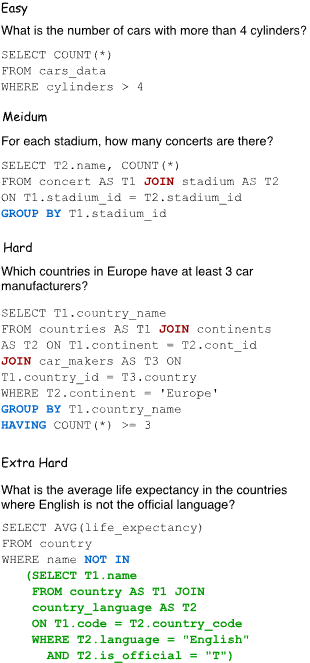
\includegraphics[width=0.35\textwidth]{image.png}
\caption{SQL query examples in 4 hardness levels. Credit: Spider (Yu et al., 2018)}
\label{fig:hardness-levels}
\end{figure}

\subsection{Prompting and Input}
\label{sec:prompting}

Each model receives three pieces of information in a single zero-shot user turn: a system instruction explaining its role as a Text-to-SQL generator, the database schema (Table names, column names, primary keys, and foreign-key relationships, with no example rows), and the natural-language question. No few-shot examples are provided, so that the experiment measures each model's ability to generate SQL from instructions and schema information alone, without the confound of examples steering its output style. The prompt template is identical across all three models, so that differences in performance can be attributed to the models rather than to differences in prompting.

\textbf{Prompt template:}
\begin{verbatim}
Given the following SQLite database schema, write a SQL query that answers
the question.

{schema}

Question: {question}

Respond with only the SQL query in a ```sql code block.
\end{verbatim}

See \hyperref[sec:appendix1]{Appendix 1} for a worked example: a full schema, a question, and the resulting filled prompt.

\subsection{SQL Extraction}
\label{sec:sql-extraction}

For each sample, we decode the model's generated tokens into text using the model-specific tokenizer, and check for the presence of a \texttt{</think>} token. If \texttt{</think>} was generated, we take all text generated before \texttt{</think>} as the reasoning trace and all text to the right as the output SQL; DeepSeek-R1-Distill-Qwen-1.5B is the only model of the three that can emit this token. The SQL is then extracted from the first \texttt{```sql} code block in that remaining text. The extracted SQL is passed to the evaluation script as-is. Outputs that cannot be extracted or parsed are counted as incorrect on every metric rather than excluded from the evaluation, as unusable output is a task failure (see \ref{sec:evaluation-metrics} and \ref{sec:invalid-outputs}).

\subsection{Inference Settings}
\label{sec:inference-settings}

All models are evaluated using the same decoding configuration: greedy decoding (temperature and top-p are not applicable) for consistent, reproducible results between runs. The maximum output length differs by model: 256 tokens for Qwen3-0.6B, and 4096 tokens for both Qwen3-4B and DeepSeek-R1-Distill-Qwen-1.5B. For DeepSeek, the larger budget is needed because its output also has to contain a full reasoning trace rather than only the SQL query; Qwen3-4B is given the same, larger budget as DeepSeek so that a tighter token limit can be ruled out as the reason for any difference between them on invalid-output rate (\ref{sec:invalid-outputs}) or inference time (\ref{sec:efficiency}). Qwen3-0.6B and Qwen3-4B are both run with thinking mode off (both support it). DeepSeek-R1-Distill-Qwen-1.5B always produces a reasoning trace and has no documented way to disable thinking mode, so it is evaluated as the reasoning condition against the two non-reasoning Qwen3 models. All inference runs on the same 1x RTX 4090 GPU described in \ref{sec:models}, with batch size 128.

\subsection{Evaluation}
\label{sec:evaluation-metrics}

We evaluate the output using the same metrics as the Spider paper (Yu et al., 2018). These are:

\begin{enumerate}
\item Component Matching
    \begin{itemize}
        \item For each of the following components:
        \begin{itemize}
            \item SELECT
            \item WHERE
            \item GROUP BY
            \item ORDER BY
            \item KEYWORDS (including all SQL keywords without column names and operators)
        \end{itemize}
        \item Decompose each component in the prediction and ground truth as bags of several sub-components and check whether or not these two sets of components match completely.
        \item Checks accuracy, recall, and F1
    \end{itemize}
\item Exact Matching Accuracy
    \begin{itemize}
        \item We measure whether the generated query as a whole is equivalent to the golden query (AKA ground truth query)
        \item The generated query is correct only if all components are correct
        \item Checks only accuracy
    \end{itemize}
\item Execution Accuracy
    \begin{itemize}
        \item A list of gold values for each question is given
        \item We measure how many gold values the generated query extracts when executed
        \item Checks only accuracy
    \end{itemize}
\end{enumerate}

If output is invalid or unparsable, then it fails exact matching and execution accuracy. Results~\ref{sec:invalid-outputs} reports how often this happens for each model.

\section{RQ1: Results}
\label{sec:rq1-results}

\subsection{Overall Model Performance}
\label{sec:overall-performance}

Below we report how Qwen3-0.6B, Qwen3-4B, and DeepSeek-R1-Distill-Qwen-1.5B perform on the Spider benchmark across all 3 metrics (Component Matching, Exact Matching Accuracy, Execution Accuracy). We calculate the values per problem difficulty as well as overall, and display them in the below tables.

\begin{table}[H]
\centering
\footnotesize
\caption{Overall performance summary, aggregated across all difficulties (all 1034 problems). Component matching is accuracy / recall / F1 (macro-averaged, see the note on Table~\ref{tab:difficulty-component} in \ref{sec:rq1-interpretation}). Per-difficulty breakdowns are in Tables~\ref{tab:difficulty-component}--\ref{tab:difficulty-execution}.}
\label{tab:overall-performance}
\resizebox{\textwidth}{!}{%
\begin{tabular}{lllccc}
\toprule
Model & Parameters & Category & Component matching & Exact matching & Execution accuracy \\
\midrule
Qwen3-0.6B & 0.6B & Decoder-only & 0.628 / 0.209 / 0.314 & 0.099 & 0.209 \\
Qwen3-4B & 4B & Decoder-only & 0.797 / 0.306 / 0.442 & 0.256 & 0.353 \\
DeepSeek-R1-Distill-Qwen-1.5B & 1.5B & Reasoning & 0.661 / 0.174 / 0.275 & 0.085 & 0.121 \\
\bottomrule
\end{tabular}}
\end{table}

All models are evaluated zero-shot with the same prompt on the 20 databases of the Spider dev set. Aggregated across all difficulties and databases, every model is still far from solving the task: execution accuracy ranges from 0.121 (DeepSeek) to 0.353 (Qwen3-4B) and exact matching accuracy from 0.085 (DeepSeek) to 0.256 (Qwen3-4B). Execution accuracy is higher than exact matching accuracy for all three models (for example 0.353 vs.\ 0.256 for Qwen3-4B), which suggests that at least some of the queries that return the correct result are written differently from the gold SQL (see Section \ref{sec:rq1-interpretation} for more on this relationship). Of the three models, Qwen3-4B is now the best on almost every metric, database, and difficulty level; Section \ref{sec:by-database} and Section \ref{sec:rq1-interpretation} quantify how consistently. Table ~\ref{tab:inference-time} reports the efficiency side of this comparison: inference time per example.

\subsection{Performance by Query Difficulty}
\label{sec:by-difficulty}

\begin{table}[H]
\centering
\footnotesize
\caption{Component matching (accuracy / recall / F1) by difficulty.}
\label{tab:difficulty-component}
\begin{tabular}{lcc}
\toprule
Model & easy & medium \\
\midrule
Problems (n) & 248 & 446 \\
Qwen3-0.6B & 0.675 / 0.308 / 0.423 & 0.582 / 0.235 / 0.334 \\
Qwen3-4B & 0.838 / 0.574 / 0.681 & 0.670 / 0.306 / 0.420 \\
DeepSeek-R1-Distill-Qwen-1.5B & 0.566 / 0.288 / 0.382 & 0.642 / 0.185 / 0.287 \\
\bottomrule
\end{tabular}

\vspace{0.5em}

\begin{tabular}{lccc}
\toprule
Model & hard & extra & all \\
\midrule
Problems (n) & 174 & 166 & 1034 \\
Qwen3-0.6B & 0.540 / 0.141 / 0.223 & 0.578 / 0.160 / 0.250 & 0.628 / 0.209 / 0.314 \\
Qwen3-4B & 0.796 / 0.262 / 0.394 & 0.485 / 0.150 / 0.229 & 0.797 / 0.306 / 0.442 \\
DeepSeek-R1-Distill-Qwen-1.5B & 0.543 / 0.113 / 0.187 & 0.389 / 0.104 / 0.164 & 0.661 / 0.174 / 0.275 \\
\bottomrule
\end{tabular}
\end{table}

\begin{table}[H]
\centering
\footnotesize
\caption{Exact matching accuracy by difficulty.}
\label{tab:difficulty-exact}
\begin{tabular}{lccccc}
\toprule
Model & easy & medium & hard & extra & all \\
\midrule
Problems (n) & 248 & 446 & 174 & 166 & 1034 \\
Qwen3-0.6B & 0.157 & 0.137 & 0.006 & 0.006 & 0.099 \\
Qwen3-4B & 0.508 & 0.262 & 0.115 & 0.012 & 0.256 \\
DeepSeek-R1-Distill-Qwen-1.5B & 0.214 & 0.078 & 0.000 & 0.000 & 0.085 \\
\bottomrule
\end{tabular}
\end{table}

\begin{table}[H]
\centering
\footnotesize
\caption{Execution accuracy by difficulty.}
\label{tab:difficulty-execution}
\begin{tabular}{lccccc}
\toprule
Model & easy & medium & hard & extra & all \\
\midrule
Problems (n) & 248 & 446 & 174 & 166 & 1034 \\
Qwen3-0.6B & 0.210 & 0.276 & 0.126 & 0.114 & 0.209 \\
Qwen3-4B & 0.565 & 0.345 & 0.276 & 0.139 & 0.353 \\
DeepSeek-R1-Distill-Qwen-1.5B & 0.258 & 0.128 & 0.017 & 0.006 & 0.121 \\
\bottomrule
\end{tabular}
\end{table}

We break every metric down by the Spider Hardness Criteria (\ref{sec:eval-data}), since aggregate numbers alone would hide whether a model's advantage holds up as queries get harder.

Performance decreases with difficulty for every model, but the decrease is steepest for Qwen3-0.6B and DeepSeek: their exact matching and execution accuracy are both at most 0.006 and 0.126 respectively on hard and extra problems, down from as high as 0.210-0.258 (easy execution) on the easiest problems (Table~\ref{tab:difficulty-exact} and Table~\ref{tab:difficulty-execution}). Qwen3-4B degrades on the same relative scale but from a much higher starting point, from 0.508 easy exact matching / 0.565 easy execution accuracy down to 0.012 extra exact matching / 0.139 extra execution accuracy. Despite the degradation, it remains the best of the three models at every single difficulty level on both metrics (Tables~\ref{tab:difficulty-exact}--\ref{tab:difficulty-execution}).

\subsection{Performance by Database}
\label{sec:by-database}

We also break execution and exact matching accuracy down by each of the 20 Spider dev databases. Qwen3-4B has the highest execution accuracy on 17 of the 20 databases outright (plus a tie on one more) and the highest exact matching accuracy on 18 of 20, while DeepSeek-R1-Distill-Qwen-1.5B is never highest on either metric; Qwen3-0.6B wins outright only on orchestra and battle\_death. Databases with few problems (real\_estate\_properties with n=4, voter\_1 with n=15, battle\_death with n=16, and museum\_visit with n=18) are too small to rank the models reliably, since a single problem changes a score by 6 to 25 percentage points. Execution accuracy ranges from 0.10 (course\_teach) to 0.53 (singer) for Qwen3-0.6B, from 0.19 (battle\_death) to 0.60 (singer) for Qwen3-4B, and from 0.00 (concert\_singer) to 0.27 (singer and voter\_1) for DeepSeek-R1-Distill-Qwen-1.5B (\hyperref[tab:db-execution]{Table 5}). 


\begin{table}[H]
\centering
\footnotesize
\caption{Execution accuracy by database (domain).}
\begin{tabular}{lcccc}
\toprule
Database & Problems (n) & Qwen3-0.6B & Qwen3-4B & DeepSeek-R1-Distill-Qwen-1.5B \\
\midrule
world\_1 & 120 & 0.183 & 0.242 & 0.108 \\
car\_1 & 92 & 0.109 & 0.315 & 0.054 \\
cre\_Doc\_Template\_Mgt & 84 & 0.202 & 0.405 & 0.071 \\
dog\_kennels & 82 & 0.159 & 0.293 & 0.085 \\
flight\_2 & 80 & 0.263 & 0.500 & 0.250 \\
student\_transcripts\_tracking & 78 & 0.128 & 0.321 & 0.064 \\
wta\_1 & 62 & 0.161 & 0.290 & 0.129 \\
tvshow & 62 & 0.339 & 0.435 & 0.129 \\
network\_1 & 56 & 0.286 & 0.375 & 0.179 \\
concert\_singer & 45 & 0.111 & 0.289 & 0.000 \\
pets\_1 & 42 & 0.167 & 0.286 & 0.071 \\
poker\_player & 40 & 0.250 & 0.550 & 0.225 \\
orchestra & 40 & 0.350 & 0.250 & 0.100 \\
employee\_hire\_evaluation & 38 & 0.105 & 0.211 & 0.132 \\
course\_teach & 30 & 0.100 & 0.500 & 0.100 \\
singer & 30 & 0.533 & 0.600 & 0.267 \\
museum\_visit & 18 & 0.278 & 0.500 & 0.222 \\
battle\_death & 16 & 0.375 & 0.188 & 0.188 \\
voter\_1 & 15 & 0.267 & 0.400 & 0.267 \\
real\_estate\_properties & 4 & 0.500 & 0.500 & 0.000 \\
\bottomrule
\label{tab:exec-acc-rq1-by-database}
\end{tabular}
\end{table}


The pattern on exact matching accuracy is just as one-sided (\hyperref[tab:db-exact]{Table 6}): Qwen3-4B is highest on 18 of 20 databases, ties Qwen3-0.6B on orchestra, and loses only on battle\_death; DeepSeek's exact matching accuracy is never the highest of the three, coming closest on flight\_2 (0.200 vs.\ Qwen3-4B's 0.350 and Qwen3-0.6B's 0.075). The full per-database tables and discussion are in \hyperref[sec:appendix2]{Appendix 2}.

\subsection{Analysis of Invalid and Unparseable Outputs}
\label{sec:invalid-outputs}

We also count how often each model's output cannot be used as SQL at all: it either never produces a usable query within the token budget (\ref{sec:inference-settings}) or is truncated before finishing one. Per \ref{sec:evaluation-metrics}, these count as failures on every metric rather than being excluded, and this is a direct measure of how reliably each model follows the ``respond with only a SQL query'' instruction, independent of whether the SQL it does produce is correct. Qwen3-0.6B's invalid rate is 2.2\%, Qwen3-4B's is 0.0\%, and DeepSeek-R1-Distill-Qwen-1.5B's is 9.7\%, about 4x higher than Qwen3-0.6B's despite having the same 4096-token budget as Qwen3-4B (\ref{sec:inference-settings}), i.e. a larger token budget did not cause Qwen3-4B to run on or produce unusable output the way it does for DeepSeek. Section \ref{sec:rq1-interpretation} breaks DeepSeek's failures down further by difficulty and by why the generation failed (see Tables~\ref{tab:deepseek-outcome}--\ref{tab:deepseek-unfinished-by-difficulty}).


\begin{table}[H]
\centering
\footnotesize
\caption{DeepSeek-R1-Distill-Qwen-1.5B by generation outcome. ``Cut'' means the generation reached the 4096-token limit.}
\label{tab:deepseek-outcome}
\begin{tabular}{lccccc}
\toprule
Outcome & Problems (n) & Share & Avg.\ tokens & Exact match & Component F1 \\
\midrule
Finished with SQL & 934 & 90.3\% & 512 & 0.094 & 0.286 \\
Finished, no usable SQL & 2 & 0.2\% & 284 & 0.000 & 0.100 \\
Cut while answering (after \texttt{</think>}) & 13 & 1.3\% & 4096 & 0.000 & 0.096 \\
Cut while thinking (no \texttt{</think>}) & 85 & 8.2\% & 4096 & 0.000 & 0.093 \\
All & 1034 & 100\% & 851 & 0.085 & 0.275 \\
\bottomrule
\end{tabular}
\end{table}

\begin{table}[H]
\centering
\footnotesize
\caption{The same 934 questions that DeepSeek finished, for all three models.}
\label{tab:deepseek-finished-934}
\begin{tabular}{lcc}
\toprule
Model & Exact match & Component F1 \\
\midrule
DeepSeek-R1-Distill-Qwen-1.5B & 0.094 & 0.286 \\
Qwen3-0.6B & 0.103 & 0.317 \\
Qwen3-4B & 0.257 & 0.440 \\
\bottomrule
\end{tabular}
\end{table}

\begin{table}[H]
\centering
\footnotesize
\caption{Share of Deepseek generations that are infinite self-repetition loops. We check self-repetition using compression ratio: a text that repeats itself compresses well, so a low compression ratio of the last 3000 characters indicates a loop. In testing, we found generations with compression ratios <0.15 infinitely self-looped.}
\label{tab:deepseek-repetition}
\begin{tabular}{lcccc}
\toprule
Generations & n & Median compression ratio & Ratio $<$ 0.15 & Last 150 characters repeat 3 or more times \\
\midrule
Cut off & 98 & 0.095 & 95.9\% & 96.9\% \\
Finished & 936 & 0.418 & 0.0\% & 0.2\% \\
\bottomrule
\end{tabular}
\end{table}

\begin{table}[H]
\centering
\footnotesize
\caption{Share of DeepSeek generations that did not finish with SQL, by difficulty.}
\label{tab:deepseek-unfinished-by-difficulty}
\begin{tabular}{lccccc}
\toprule
 & easy & medium & hard & extra & all \\
\midrule
Problems (n) & 248 & 446 & 174 & 166 & 1034 \\
Not finished with SQL (n) & 15 & 33 & 25 & 27 & 100 \\
Share & 6.0\% & 7.4\% & 14.4\% & 16.3\% & 9.7\% \\
\bottomrule
\end{tabular}
\end{table}

\subsection{Efficiency Measures}
\label{sec:efficiency}

\begin{table}[H]
\centering
\footnotesize
\caption{Output tokens per example.}
\label{tab:tokens-per-example}
\begin{tabular}{lccccc}
\toprule
Model & easy & medium & hard & extra & all \\
\midrule
Qwen3-0.6B & 27.5 & 44.7 & 53.7 & 69.9 & 46.1 \\
Qwen3-4B & 23.6 & 37.3 & 46.2 & 59.0 & 39.0 \\
DeepSeek-R1-Distill-Qwen-1.5B & 610.8 & 768.4 & 1096.0 & 1176.9 & 851.3 \\
\bottomrule
\end{tabular}
\end{table}

Inference time is measured from the start of generation to the complete batch output, per batch of 128 examples, with each batch's wall time divided evenly across its 128 examples to get the per-example figure, excluding tokenization, model loading, and warm-up.

\begin{table}[H]
\centering
\footnotesize
\caption{Inference time.}
\label{tab:inference-time}
\begin{tabular}{lcc}
\toprule
Model & Total wall time (s) & Avg.\ time per example (s) \\
\midrule
Qwen3-0.6B & 123.9 & 0.120 \\
Qwen3-4B & 109.1 & 0.106 \\
DeepSeek-R1-Distill-Qwen-1.5B & 3059.8 & 2.959 \\
\bottomrule
\end{tabular}
\end{table}

DeepSeek is about 25x slower per example than Qwen3-0.6B and 28x slower than Qwen3-4B, consistent with its much higher average token count (Table~\ref{tab:tokens-per-example}). Qwen3-4B, despite having about 7x as many parameters as Qwen3-0.6B, is marginally faster per example (0.106s vs.\ 0.120s), consistent with it generating fewer tokens on average (39.0 vs.\ 46.1, Table~\ref{tab:tokens-per-example}) despite having the same 16x larger token budget as DeepSeek (\ref{sec:inference-settings}).


\section{RQ1: Interpretation and Answer}
\label{sec:rq1-interpretation}

\textbf{RQ1:} How do (selected) LLMs perform on cross-domain Text-to-SQL?

\vspace{10px}

All three models are still far from solving the task in this zero-shot setting: exact matching accuracy ranges from 0.085 to 0.256 and execution accuracy from 0.121 to 0.353 (Table~\ref{tab:overall-performance}). Difficulty and database effects are discussed in \ref{sec:by-difficulty} and \ref{sec:by-database}; here we interpret the effects of model size and reasoning architecture and the exact-match/execution-accuracy relationship, and state the answer to RQ1 as three findings.

\subsection{First, within the Qwen family, scale is a strong and almost uniform predictor of performance, but an intermediate-size reasoning model from the DeepSeek family still loses to the smallest model in the Qwen family.}
\label{sec:rq1-finding-scale}

Aggregated across all difficulties, Qwen3-4B has the best component matching (0.797 accuracy / 0.306 recall / 0.442 F1), exact matching (0.256 ), and execution accuracy (0.353) of the three (Table~\ref{tab:overall-performance}), and it beats Qwen3-0.6B on exact matching and execution accuracy at every individual difficulty level, including hard (0.115 vs.\ 0.006) and extra (0.012 vs.\ 0.006), where the smaller model solves almost nothing (Tables~\ref{tab:difficulty-exact}--\ref{tab:difficulty-execution}). This effect is large and holds at every difficulty level. The one exception is component matching on extra-hard problems, where Qwen3-0.6B's accuracy, recall, and F1 (0.578 / 0.160 / 0.250) are all slightly higher than Qwen3-4B's (0.485 / 0.150 / 0.229), the only point in the RQ1 results where the smaller Qwen3 model wins outright (Table~\ref{tab:difficulty-component}). DeepSeek-R1-Distill-Qwen-1.5B sits between the two Qwen3 models in parameter count (1.5B) and is the only one that reasons, yet it is the lowest of the three on every aggregate metric (0.275 component F1, 0.085 exact matching, 0.121 execution accuracy) except its own component-matching accuracy (0.661 vs.\ 0.628 for Qwen3-0.6B). Thus, scale predicts performance well within a family, but does not transfer across the reasoning/non-reasoning boundary: having more parameters than Qwen3-0.6B did not help DeepSeek catch up to it.

\subsection{Second, the reasoning architecture itself, not parameter count, is the most likely driver of DeepSeek's low score.}
\label{sec:rq1-finding-reasoning}

Its invalid-output rate (9.7\%) is markedly higher than Qwen3-0.6B's (2.2\%) and Qwen3-4B's (0.0\% in this run) (\ref{sec:invalid-outputs}). In Tables~\ref{tab:deepseek-outcome}--\ref{tab:deepseek-unfinished-by-difficulty}, 100 of 1034 generations (9.7\%) end without usable SQL. 85 never leave the reasoning phase, 13 are cut while writing the answer, and 2 finish without SQL. The number of unusable SQL generations also grows with difficulty, from 6.0\% on easy to 16.3\% on extra problems. These are not cases of long productive reasoning either: 95.9\% of the cut-off generations are highly self-repetitive (compression ratio below 0.15, median compression ratio 0.095, vs.\ 0.418 for finished generations), rewriting the same query and repeating phrases like ``So the final query is:'' without converging. Finishing does not make it better either: on the 934 questions DeepSeek does finish, its exact matching (0.094) and component F1 (0.286) are still below Qwen3-0.6B's on the same questions (0.103 / 0.317) and far below Qwen3-4B's (0.257 / 0.440), despite generating 512 tokens per question on average there, against 46 and 39 tokens overall for Qwen3-0.6B and Qwen3-4B (about 11x and 13x fewer). This extra length also costs time: DeepSeek is 25-28x slower per example than either Qwen3 model (\ref{sec:efficiency}). The reasoning trace mostly lengthens the output and sometimes never terminates, without improving the SQL when it does, and size alone is not the explanation, since Qwen3-4B is both bigger than DeepSeek and the best model in the comparison. This does not fully isolate reasoning from DeepSeek's other differences from the two Qwen3 models, such as distillation (see Limitations).

\subsection{Third, query difficulty has a substantial, consistent effect on every model, including the best one.}
\label{sec:rq1-finding-difficulty}

Exact matching and execution accuracy both fall sharply from easy to extra-hard problems for all three models (\ref{sec:by-difficulty}). Qwen3-4B's drop is from a much higher base (0.508 to 0.012 exact matching, 0.565 to 0.139 execution accuracy) and it remains the best model at every difficulty level on both metrics, but the drop itself is just as steep in relative terms as for the other two models, and the hardest problems remain largely unsolved even for it.

\subsection{Exact Match vs.\ Execution Accuracy}
\label{sec:rq1-exact-vs-execution}

For all three models, execution accuracy aggregated across all difficulties exceeds exact matching accuracy (Table~\ref{tab:overall-performance}): 0.209 vs.\ 0.099 for Qwen3-0.6B, 0.353 vs.\ 0.256 for Qwen3-4B, and 0.121 vs.\ 0.085 for DeepSeek. Since exact matching requires every SQL component to match the gold query while execution accuracy only requires the same result set, this gap indicates each model writes some queries that are valid and correct but phrased differently from the gold SQL (e.g.\ a different but equivalent join order, or an explicit column list where the gold query uses \texttt{SELECT *}). The gap is widest for Qwen3-0.6B (11.0 points), close behind for Qwen3-4B (9.7 points), and narrowest for DeepSeek (3.6 points); DeepSeek's narrower gap reflects it producing fewer alternative-but-valid queries. Qwen3-4B's gap is almost as wide as Qwen3-0.6B's despite much higher absolute accuracy, so scaling up within the Qwen3 family raises both exact matching accuracy and execution accuracy together rather than closing the gap between them.

\subsection{Limitations}
\label{sec:rq1-limitations}

Our working hypothesis is that Text-to-SQL at this scale does not benefit from an explicit reasoning trace, and that a non-reasoning model is sufficient, with performance instead scaling with parameter count within a fixed model family. The results are consistent with this hypothesis. However, they do not establish that Text-to-SQL is too simple for reasoning models in general due to several factors:

\begin{itemize}
\item \textbf{Model differences beyond reasoning.} Qwen3-0.6B and Qwen3-4B share a model family, isolating the effect of scale between them, but DeepSeek differs from both in family, size, and pretraining/post-training, not only in whether it reasons; it is also a distilled model, so the effect of reasoning cannot be fully separated from distillation quality.
\item \textbf{Aggregated component matching.} The component matching figures in Table~\ref{tab:difficulty-component} (and in Table~\ref{tab:overall-performance}) are our own macro-average (mean of the 10 per-component accuracy and recall scores, with F1 computed from these two means), not a number reported by Spider.
\end{itemize}

Overall, in this zero-shot, cross-domain setting, a larger non-reasoning decoder-only model (Qwen3-4B, 4B) clearly outperforms both a same-family model at under a sixth its size (Qwen3-0.6B) and a reasoning model of intermediate size from a different family (DeepSeek-R1-Distill-Qwen-1.5B, 1.5B), while also being faster per example than either. None of the three models solve more than half of even the easiest problems or more than a small fraction of hard or extra-hard queries. This answers RQ1 for the three models evaluated. (this
% file's cross-references into Task 1 -- table~\ref{tab:deepseek-outcome},
% \ref{tab:tokens-per-example}, \ref{sec:sql-extraction}, etc. -- rely on
% RQ1.tex's labels already being defined earlier in the same document).
%
% Structure: Methodology is organized per-feature (Feature 1: Token Count,
% Feature 2: Information Retention), each with its own Definition / Why it's
% relevant / How we computed it. Results is organized as descriptive
% statistics, differences by correctness, differences by difficulty, and
% relationship with Text-to-SQL correctness (the correlation analysis).

\section{Task 2 -- RQ2: Methodology}
\label{sec:rq2-methodology}

\textbf{RQ2:} How do characteristics of reasoning traces (of reasoning LLM) relate to Text-to-SQL performance?

To answer this question, we examine two features of each reasoning trace: Token Count and Information Retention. We compute both for all 1034 generations in DeepSeek-R1-Distill-Qwen-1.5B's main Task 1 run, then relate each to difficulty and to Text-to-SQL correctness.

\subsection{Feature 1: Token Count}
\label{sec:rq2-feature-tokencount}

\textbf{Definition.} Token Count is the number of tokens in the reasoning segment of a generation, i.e.\ everything the model generates before \texttt{</think>}, excluding the final SQL answer. We split each generation into a reasoning segment and an answer segment using the same \texttt{</think>} split used in Task 1 (\ref{sec:sql-extraction}).

% We hypothesize that for each difficulty there exists a "goldilocks" token-count range, and that performance improves as the answer's token count approaches the mean of that range.

\textbf{Why it's relevant.} Examining token count allows us to investigate whether the amount of generated reasoning is associated with better Text-to-SQL performance. However, a longer trace does not necessarily mean better reasoning, since additional tokens may contain redundant or irrelevant information.

Additionally, we expect Token Count to scale positively with the difficulty of the related Text-to-SQL problem: easy questions should require fewer thinking tokens, while extra-hard questions should require significantly more. Any question that disobeys this relation, or where more tokens associate with worse rather than better answers, is given special attention in Results.

\textbf{How we computed it.} Token Count is the number of tokens in the reasoning segment only, re-tokenized with the model's own tokenizer (not the \texttt{new\_tokens} field logged during generation, which counts the whole generation, reasoning plus SQL). For generations that never emit \texttt{</think>} (truncated at the 4096-token generation limit, see Task 1's table~\ref{tab:deepseek-outcome}), the entire generated text is treated as the reasoning segment, so Token Count for these rows is effectively capped at the generation limit rather than reflecting a completed thought. This is intentional: these cases are exactly the repetition loops Task 1 identified (table~\ref{tab:deepseek-repetition}), and dropping them would hide, rather than explain, the heavy right tail in Token Count. We keep them in the Token Count analysis and flag wherever they drive a result (see finding~\ref{item:rq2-finding-tokencount-difficulty} in Results).

\begin{table}[H]
\centering
\footnotesize
\caption{Token Count: definition and computation summary.}
\label{tab:rq2-feature-tokencount-summary}
\begin{tabular}{p{0.22\textwidth}p{0.7\textwidth}}
\toprule
Property & Detail \\
\midrule
Unit & Tokens (model's own tokenizer) \\
Scope & Reasoning segment only, i.e.\ text before \texttt{</think>} \\
Range & Non-negative integer, long right tail (observed 103--4166) \\
Truncated traces & Treated as reasoning segment in full; capped at the 4096-token generation limit \\
\bottomrule
\end{tabular}
\end{table}

\subsection{Feature 2: Information Retention}
\label{sec:rq2-feature-retention}

\textbf{Definition.} Information Retention is the share of schema-shaped identifiers mentioned in a reasoning trace that actually exist as a table or column name in that question's schema. Equivalently, $$(1-\text{Information Retention})=\text{fraction of mentioned identifiers that are not grounded in the prompt}$$ or in other words, the hallucination rate of the trace.

\textbf{Why it's relevant.} We expect reasoning traces with low Information Retention (frequent hallucination of schema elements) to produce lower-performing answers than traces that stay grounded in the given schema, since inventing a table or column that doesn't exist is very likely to propagate into an incorrect query. We also expect harder problems to not cause lower Information Retention on their own; if they do, this points to the model introducing more assumptions as questions get harder, which is itself worth investigating as a bias rather than attributing the accuracy drop to difficulty alone.

\textbf{How we computed it.} We regex-extract every schema-shaped identifier the trace mentions, either quoted (e.g.\ \texttt{"Singer\_ID"}) or underscore-joined (e.g.\ \texttt{concert\_id}), and take the share of those identifiers that match a table or column name in that question's schema. An identifier that matches neither is treated as a fact the model introduced on its own, i.e., a hallucination. Traces that mention no schema identifiers at all are excluded from Information Retention (but kept for Token Count), since a 0-of-0 ratio is undefined rather than evidence of perfect or zero retention; this drops the usable sample from 1034 to 1017.

\begin{table}[H]
\centering
\footnotesize
\caption{Information Retention: definition and computation summary.}
\label{tab:rq2-feature-retention-summary}
\begin{tabular}{p{0.22\textwidth}p{0.7\textwidth}}
\toprule
Property & Detail \\
\midrule
Unit & Ratio, bounded in $[0,1]$ \\
Numerator & Schema identifiers mentioned in the trace that match a real table/column name \\
Denominator & All schema-shaped identifiers mentioned in the trace (quoted or underscore-joined) \\
Exclusions & Traces mentioning zero schema identifiers (1034 $\rightarrow$ 1017 usable rows) \\
Truncated traces & Scored over the partial text generated before truncation \\
\bottomrule
\end{tabular}
\end{table}

\subsection{Statistical approach}
\label{sec:rq2-statistical-approach}

We relate both Token Count and Information Retention to correctness and difficulty with Spearman's Rank Correlation throughout. Both of our hypotheses are about monotonic relationships, not linear relationships (performance should not decrease as Token Count or Information Retention increase, and Token Count should increase with difficulty), which is exactly what Spearman's Rank Correlation tests for. It also suits the distribution of our two reasoning metrics: Token Count is a non-negative count with a long right tail (DeepSeek alone ranges from 611 tokens on easy problems to 1177 on extra, table~\ref{tab:tokens-per-example}), and Information Retention is a bounded ratio, so neither is likely to be symmetric and unbounded; the $\geq$90\% trace completion rate gives us enough data per stratum to check this on histograms rather than assume it. For correctness, we correlate each reasoning metric against the continuous, per-question component matching accuracy, recall, and F1 for all ten Spider components individually, plus exact matching and execution accuracy.

This gives 32 submetrics per reasoning metric per difficulty level. With 169 correlation tests run in total, we correct for multiple comparisons with the Benjamini-Hochberg procedure rather than a stricter family-wise correction like Bonferroni: we are screening many related, non-independent submetrics for the strongest associations to report and discuss, not making a small number of pre-registered confirmatory claims, so controlling the expected false-discovery rate is a better fit than controlling the probability of any single false positive at the cost of statistical power.

% The Results below report Token Count and Information Retention broken down two ways: by difficulty, since that is the primary hypothesis under test, and by exact-match correctness (correct/incorrect), used for the descriptive statistics and the boxplots (figure~\ref{fig:rq2-boxplots}) because a binary split is easier to read in a table or figure than 32 continuous submetrics. The correlation analysis itself (table~\ref{tab:rq2-correlations}) still uses the continuous submetrics described above, for the statistical-power reasons given there; the binary-correctness view and the continuous-submetric view are two presentations of the same underlying data, not two different analyses.

The Results below report Token Count and Information Retention by correctness and difficulty level, with the continuous submetrics used directly in the correlation analysis (Table~\ref{tab:rq2-correlations}).


\section{RQ2: Results}
\label{sec:rq2-results}

We compute Token Count and Information Retention for all 1034 generations in DeepSeek-R1-Distill-Qwen-1.5B's main Task 1 run, and correlate each against difficulty and against all 32 per-question performance submetrics as described in the Methodology. Tables ~\ref{tab:rq2-descriptive-stats-tokencount-difficulty}, ~\ref{tab:rq2-descriptive-stats-tokencount-correctness}, ~\ref{tab:rq2-descriptive-stats-retention-difficulty}, and~\ref{tab:rq2-descriptive-stats-retention-correctness} give descriptive statistics for each feature by difficulty and by exact-match correctness; figure~\ref{fig:rq2-boxplots} shows the resulting distributions; table~\ref{tab:rq2-correlations} lists the strongest correlations.

\subsection{Descriptive statistics}
\label{sec:rq2-descriptive-stats}


\begin{table}[H]
\centering
\footnotesize
\caption{Token Count descriptive statistics, by difficulty.}
\label{tab:rq2-descriptive-stats-tokencount-difficulty}
\begin{tabular}{lcccccc}
\toprule
Group & n & mean & median & std & min & max \\
\midrule
easy & 248 & 542.3 & 329.0 & 845.2 & 103 & 4096 \\
medium & 446 & 648.2 & 374.0 & 925.7 & 191 & 4166 \\
hard & 174 & 939.2 & 425.0 & 1246.2 & 226 & 4096 \\
extra & 166 & 901.6 & 434.5 & 1199.9 & 222 & 4096 \\
\midrule
all & 1034 & 712.4 & 383.0 & 1026.2 & 103 & 4166 \\
\bottomrule
\end{tabular}
\end{table}

\begin{table}[H]
\centering
\footnotesize
\caption{Token Count descriptive statistics, by exact-match correctness (1 = exact match, 0 = not).}
\label{tab:rq2-descriptive-stats-tokencount-correctness}
\begin{tabular}{lcccccc}
\toprule
Group & n & mean & median & std & min & max \\
\midrule
exact match = 0 & 946 & 748.1 & 394.0 & 1065.6 & 103 & 4166 \\
exact match = 1 & 88 & 329.3 & 314.5 & 97.7 & 195 & 849 \\
\midrule
all & 1034 & 712.4 & 383.0 & 1026.2 & 103 & 4166 \\
\bottomrule
\end{tabular}
\end{table}

\begin{table}[H]
\centering
\footnotesize
\caption{Information Retention descriptive statistics, by difficulty. Excludes traces that mention no schema identifiers (n drops from 1034 to 1017 overall).}
\label{tab:rq2-descriptive-stats-retention-difficulty}
\begin{tabular}{lcccccc}
\toprule
Group & n & mean & median & std & min & max \\
\midrule
easy & 246 & 0.915 & 1.0 & 0.146 & 0.0 & 1.0 \\
medium & 441 & 0.905 & 1.0 & 0.148 & 0.0 & 1.0 \\
hard & 172 & 0.877 & 1.0 & 0.163 & 0.0 & 1.0 \\
extra & 158 & 0.861 & 1.0 & 0.215 & 0.0 & 1.0 \\
\midrule
all & 1017 & 0.896 & 1.0 & 0.163 & 0.0 & 1.0 \\
\bottomrule
\end{tabular}
\end{table}

\begin{table}[H]
\centering
\footnotesize
\caption{Information Retention descriptive statistics, by exact-match correctness (1 = exact match, 0 = not). Excludes traces that mention no schema identifiers (n drops from 1034 to 1017 overall).}
\label{tab:rq2-descriptive-stats-retention-correctness}
\begin{tabular}{lcccccc}
\toprule
Group & n & mean & median & std & min & max \\
\midrule
exact match = 0 & 931 & 0.893 & 1.0 & 0.166 & 0.0 & 1.0 \\
exact match = 1 & 86 & 0.924 & 1.0 & 0.123 & 0.5 & 1.0 \\
\midrule
all & 1017 & 0.896 & 1.0 & 0.163 & 0.0 & 1.0 \\
\bottomrule
\end{tabular}
\end{table}


\begin{figure}[H]
\centering
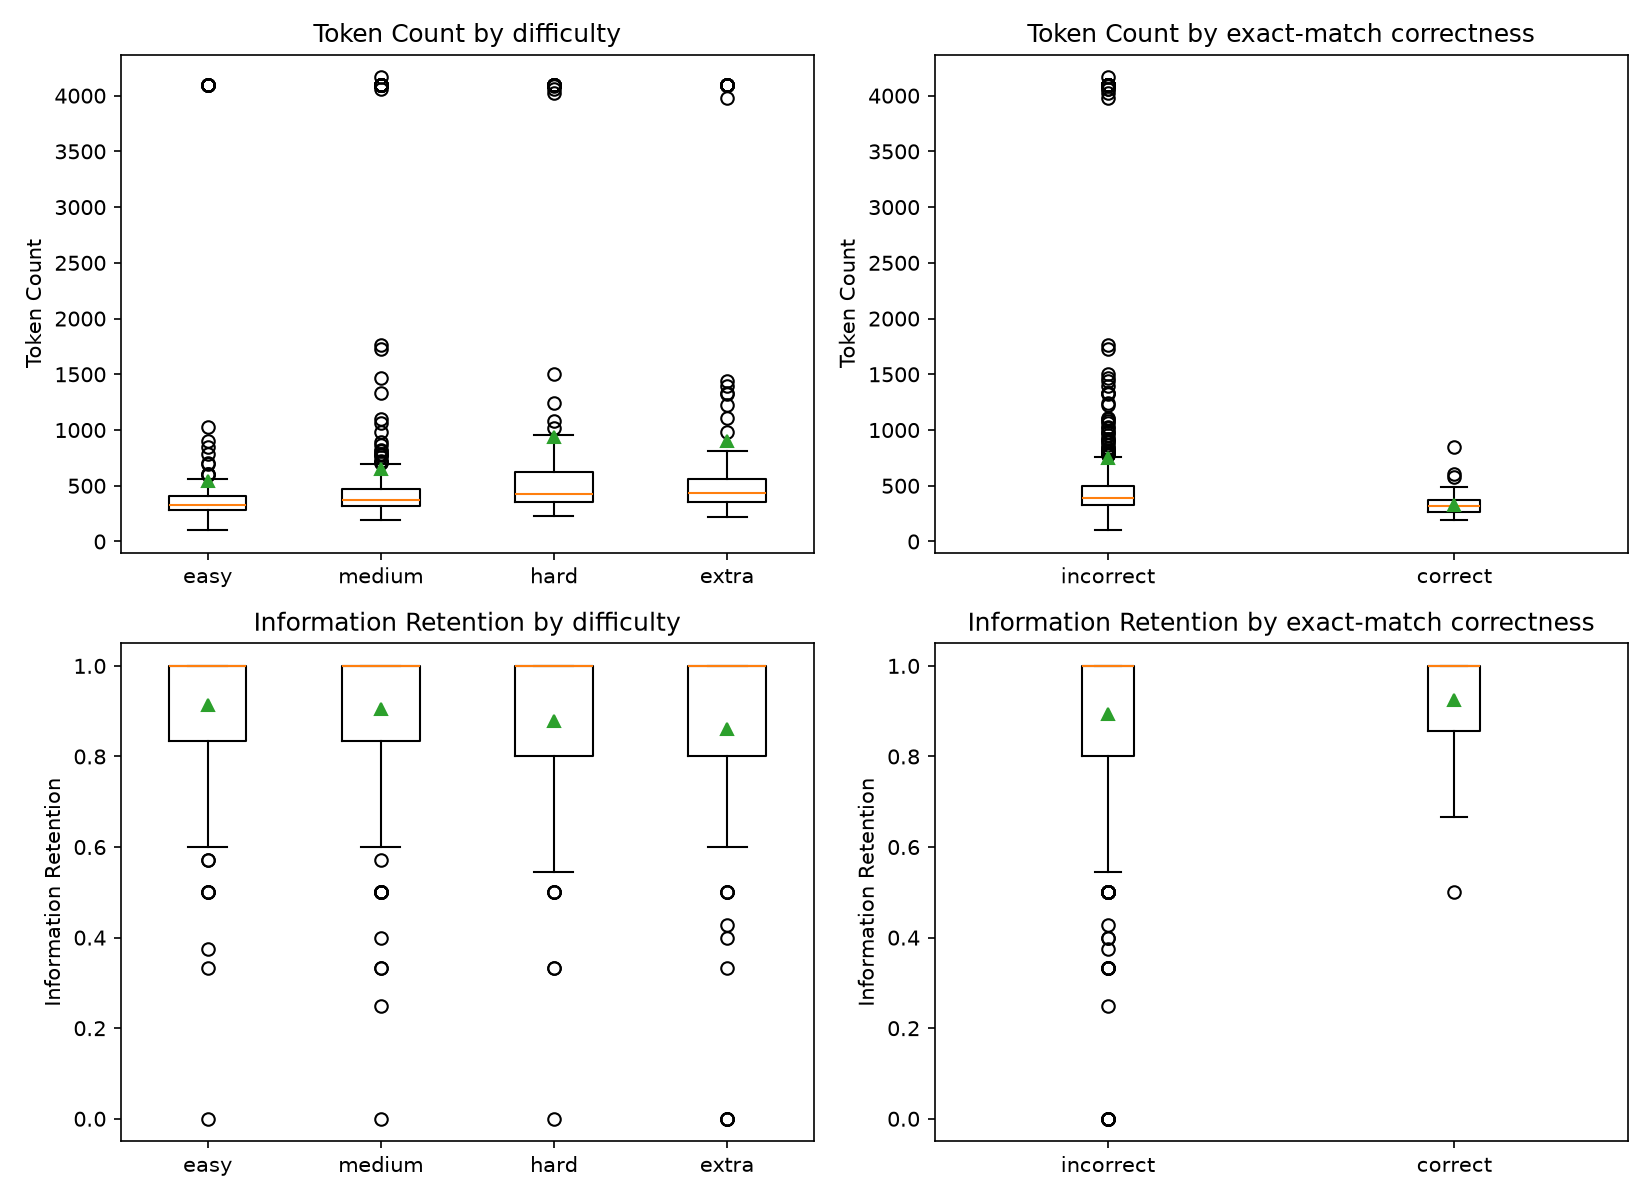
\includegraphics[width=0.85\textwidth]{boxplots.png}
\caption{Token Count and Information Retention by difficulty and by exact-match correctness, for DeepSeek-R1-Distill-Qwen-1.5B's 1034 Task 1 generations. Green triangles are means, orange lines are medians. Means sit well above medians throughout, confirming the right-skewed, bounded distributions the Methodology assumes rather than normal ones.}
\label{fig:rq2-boxplots}
\end{figure}

\subsection{Differences by correctness}
\label{sec:rq2-by-correctness}

Correct generations (exact match = 1) have a much lower mean and tighter spread of Token Count (329.3, std 97.7) than incorrect ones (748.1, std 1065.6, table~\ref{tab:rq2-descriptive-stats-tokencount-correctness}), and a slightly higher mean Information Retention (0.924 vs.\ 0.893, table~\ref{tab:rq2-descriptive-stats-retention-correctness}). Both differences point the same direction as the correlation findings in \ref{sec:rq2-relationship-correctness}: more reasoning tokens and lower retention associate with worse performance. The gap is far larger for Token Count than for Information Retention: incorrect generations' Token Count std (1065.6) is more than ten times that of correct generations (97.7), driven by the truncated, repetition-loop traces described in \ref{sec:rq2-feature-tokencount}, almost none of which are exact matches. Information Retention's median is 1.0 in both correctness groups, so the correctness gap in retention lives entirely in the mean and the lower tail, not in a shift of the typical trace. Overall, correctness tracks Token Count far more strongly than it tracks Information Retention, both in effect size and in where the gap shows up in the distribution.

\subsection{Differences by difficulty}
\label{sec:rq2-by-difficulty}

\begin{enumerate}
\item \label{item:rq2-finding-tokencount-difficulty} \textbf{Token Count increases with difficulty, as hypothesized, but the increase is driven by a heavy tail.} Median token count rises from 329 (easy) to 374 (medium) to 425 (hard) to 434 (extra), and the correlation with difficulty is positive and significant ($\rho=0.313$, $q<0.001$). The mean rises faster than the median at every level (for example 542 vs.\ 329 on easy), because generations hitting the 4096-token limit occur at every difficulty (figure~\ref{fig:rq2-boxplots}, top row); these are the same repetition loops Task 1 identified, not productive extra reasoning on harder problems.
\item \label{item:rq2-finding-retention-difficulty} \textbf{Information Retention decreases slightly with difficulty.} Median retention is 1.0 at every difficulty level, but the mean falls from 0.915 (easy) to 0.861 (extra), and the correlation with difficulty is negative and significant ($\rho=-0.107$, $q=0.013$). This is the case flagged in \ref{sec:rq2-feature-retention} as calling for closer examination of the model's introduced assumptions on harder problems.
\end{enumerate}

\subsection{Relationship with Text-to-SQL}
\label{sec:rq2-relationship-correctness}

\begin{enumerate}
\item \label{item:rq2-finding-tokencount-disobey} \textbf{On easy and medium problems, higher Token Counts track worse performance.} Token Count correlates negatively with \texttt{keywords} F1 on easy ($\rho=-0.42$, $q<0.001$) and medium ($\rho=-0.19$, $q<0.001$) problems, and with \texttt{where} and \texttt{where(no OP)} F1 on easy problems ($\rho=-0.32$ and $-0.33$, $q<0.001$). Knowing token count increases with difficulty (see ~\ref{sec:rq2-by-difficulty}), the extra tokens on these problems look like run-away generation rather than helpful deliberation.
\item \label{item:rq2-finding-retention-performance} \textbf{Where Information Retention relates to performance, it is mostly positive, as hypothesized.} On medium problems, Information Retention correlates positively with \texttt{where} and \texttt{where(no OP)} F1 ($\rho=0.345$, $q<0.001$ for both). Of its 82 submetric tests, 8 remain significant after Benjamini-Hochberg correction, 7 positive and 1 negative (\texttt{where(no OP)} recall on easy problems, $\rho=-0.261$, $q=0.042$).

\begin{table}[H]
\centering
\footnotesize
\caption{Strongest Spearman correlations between reasoning metrics and performance submetrics, Benjamini-Hochberg corrected, top 8 of 169 tests by q-value.}
\label{tab:rq2-correlations}
\begin{tabular}{llcccc}
\toprule
Metric & Submetric & Difficulty & n & $\rho$ & $q$ \\
\midrule
Token Count & difficulty (overall) & all & 1034 & 0.313 & $<$0.001 \\
Information Retention & \texttt{where} F1 & medium & 441 & 0.345 & $<$0.001 \\
Information Retention & \texttt{where(no OP)} F1 & medium & 441 & 0.345 & $<$0.001 \\
Token Count & \texttt{keywords} F1 & easy & 248 & -0.417 & $<$0.001 \\
Token Count & \texttt{where(no OP)} F1 & easy & 248 & -0.332 & $<$0.001 \\
Token Count & \texttt{where} F1 & easy & 248 & -0.322 & $<$0.001 \\
Token Count & \texttt{keywords} F1 & medium & 446 & -0.194 & $<$0.001 \\
Information Retention & difficulty (overall) & all & 1017 & -0.107 & 0.013 \\
\bottomrule
\end{tabular}
\end{table}

% \subsection{Verification: regression controlling for confounds}
% \label{sec:rq2-robustness}

% Sections~\ref{sec:rq2-by-difficulty} and~\ref{sec:rq2-relationship-correctness} test each feature against performance one at a time, but Token Count, Information Retention, and difficulty are not independent of one another: a bivariate finding there could really be driven by one of the other two variables rather than by the feature itself. The regressions below fit all three predictors jointly as statistical models, so each coefficient reflects that predictor's relationship with the outcome after the parts explained by the other two are removed, directly checking whether the findings above survive or are confounded.

% \begin{table}[H]
% \centering
% \footnotesize
% \caption{Logistic regression: exact match on standardized log Token Count, standardized Information Retention, and standardized difficulty, fit jointly ($n=1017$, pseudo $R^2=0.188$). OR is the odds ratio per one-SD increase in the predictor.}
% \label{tab:rq2-logistic}
% \begin{tabular}{lccccc}
% \toprule
% Predictor & coef & SE & $z$ & $p$ & OR [95\% CI] \\
% \midrule
% Intercept & -3.351 & 0.227 & -14.76 & $<$0.001 & 0.035 [0.022, 0.055] \\
% log Token Count ($z$) & -1.087 & 0.300 & -3.62 & $<$0.001 & 0.337 [0.187, 0.607] \\
% Information Retention ($z$) & 0.091 & 0.139 & 0.65 & 0.514 & 1.095 [0.834, 1.437] \\
% Difficulty ($z$) & -1.278 & 0.201 & -6.35 & $<$0.001 & 0.279 [0.188, 0.413] \\
% \bottomrule
% \end{tabular}
% \end{table}

% \begin{table}[H]
% \centering
% \footnotesize
% \caption{Proportional-odds (ordinal) regression: difficulty on standardized log Token Count and standardized Information Retention, fit jointly ($n=1017$). OR is the odds ratio per one-SD increase in the predictor.}
% \label{tab:rq2-ordinal}
% \begin{tabular}{lccccc}
% \toprule
% Predictor & coef & SE & $z$ & $p$ & OR [95\% CI] \\
% \midrule
% log Token Count ($z$) & 0.398 & 0.059 & 6.78 & $<$0.001 & 1.489 [1.327, 1.670] \\
% Information Retention ($z$) & -0.177 & 0.059 & -2.99 & 0.003 & 0.837 [0.746, 0.941] \\
% \bottomrule
% \end{tabular}
% \end{table}

% Controlling for the other feature and for difficulty changes which bivariate relationship survives. Token Count's association with correctness holds up: each one-SD increase in log Token Count is associated with 66\% lower odds of an exact match (OR$=0.337$, $p<0.001$), holding Information Retention and difficulty fixed (table~\ref{tab:rq2-logistic}) --- consistent with, and strengthening, finding~\ref{item:rq2-finding-tokencount-disobey}. Information Retention's association with correctness does not survive the same control (OR$=1.095$, $p=0.514$): once Token Count and difficulty are accounted for, Retention has no detectable independent effect on correctness, so the positive finding in \ref{item:rq2-finding-retention-performance} should be read as a submetric-specific, not a global, relationship. Both features' difficulty relationships, in contrast, are independent of one another: the ordinal regression finds Token Count still predicts higher difficulty (OR$=1.489$ per SD, $p<0.001$) and Information Retention still predicts lower difficulty (OR$=0.837$ per SD, $p=0.003$) when controlling for each other (table~\ref{tab:rq2-ordinal}), so neither difficulty trend in \ref{sec:rq2-by-difficulty} is simply a byproduct of the other feature's trend.

% \subsection{Regression diagnostics}
% \label{sec:rq2-diagnostics}

% The regressions in~\ref{sec:rq2-robustness} are only as trustworthy as their assumptions: if the three predictors are collinear, or if the ordinal model's proportional-odds assumption doesn't hold, the coefficients and significance levels reported there could be misleading rather than reflecting genuine independent effects. The checks below test both before those results are treated as confirmed.

% \begin{table}[H]
% \centering
% \footnotesize
% \caption{Variance inflation factors for the three predictors in the logistic regression (table~\ref{tab:rq2-logistic}).}
% \label{tab:rq2-vif}
% \begin{tabular}{lc}
% \toprule
% Predictor & VIF \\
% \midrule
% log Token Count ($z$) & 1.057 \\
% Information Retention ($z$) & 1.020 \\
% Difficulty ($z$) & 1.059 \\
% \bottomrule
% \end{tabular}
% \end{table}

% \begin{table}[H]
% \centering
% \footnotesize
% \caption{Proportional-odds check: the pooled ordinal-regression coefficient (table~\ref{tab:rq2-ordinal}) against three separately-fit cumulative-logit models, one per difficulty cutoff. Large, systematic drift across cutoffs would indicate the proportional-odds assumption does not hold.}
% \label{tab:rq2-po-check}
% \begin{tabular}{lcccc}
% \toprule
% Cutoff & coef (Token Count) & SE & coef (Retention) & SE \\
% \midrule
% pooled (proportional-odds) & 0.398 & 0.059 & -0.177 & 0.059 \\
% $P(\text{difficulty} \geq \text{medium})$ & 0.576 & 0.117 & -0.128 & 0.081 \\
% $P(\text{difficulty} \geq \text{hard})$ & 0.396 & 0.066 & -0.195 & 0.067 \\
% $P(\text{difficulty} \geq \text{extra})$ & 0.271 & 0.074 & -0.193 & 0.078 \\
% \bottomrule
% \end{tabular}
% \end{table}

% The three predictors in the logistic regression are not meaningfully collinear (all VIF $\approx 1.0$--$1.06$, well below the common rule-of-thumb threshold of 5, table~\ref{tab:rq2-vif}), so the coefficient estimates and significance levels reported in \ref{sec:rq2-robustness} are not an artifact of Token Count, Information Retention and difficulty standing in for one another. The proportional-odds check is more mixed. Information Retention's cumulative-logit coefficient is stable across all three cutoffs ($-0.128$, $-0.195$, $-0.193$, table~\ref{tab:rq2-po-check}), consistent with the pooled $-0.177$ and with the proportional-odds assumption holding for this feature. Token Count's coefficient, however, declines monotonically across cutoffs (0.576 at the easy/medium boundary, down to 0.271 at the hard/extra boundary): Token Count distinguishes difficulty levels well at the low end but loses discriminative power at the high end, a mild violation of the proportional-odds assumption that the single pooled coefficient in table~\ref{tab:rq2-ordinal} averages over. This does not overturn the ordinal regression's conclusion that Token Count predicts difficulty (every individual cutoff coefficient is still positive and more than 3 standard errors from zero), but it means the pooled OR$=1.489$ should be read as an average effect across difficulty levels rather than a uniform one.
 into main.tex, after \usepackage{upquote}

\section{Task 1 -- RQ1: Methodology \& Results}
\label{sec:rq1-methods}

\textbf{RQ1:} How do (selected) LLMs perform on cross-domain Text-to-SQL?


\subsection{Models}
\label{sec:models}

We compare two decoder-only LLMs from the same model family at different scales (Qwen3-0.6B and Qwen3-4B) against one reasoning LLM, so that the comparison isolates the effect of scale within a fixed family from the effect of an explicit reasoning trace, as much as a 3-model study can. All three are accessed as local inference over their bf16 Huggingface checkpoints on 1x NVIDIA GeForce RTX 4090 GPU (no API-based models), so that inference parameters are fully under our control (see \ref{sec:inference-settings}).

\begin{table}[H]
\centering
\footnotesize
\caption{Models compared in RQ1.}
\label{tab:models}
\resizebox{\textwidth}{!}{%
\begin{tabular}{llllll}
\toprule
Model & Category & Parameters & Quantization & Access & Thinking mode \\
\midrule
Qwen3-0.6B (Qwen Team, 2025) & Decoder-only & 0.6B & bf16 (none beyond release precision) & Local, Huggingface checkpoint & Disabled \\
Qwen3-4B (Qwen Team, 2025) & Decoder-only & 4B & bf16 (none beyond release precision) & Local, Huggingface checkpoint & Disabled \\
DeepSeek-R1-Distill-Qwen-1.5B (DeepSeek-AI, 2025) & Reasoning & 1.5B & bf16 (none beyond release precision) & Local, Huggingface checkpoint & Always on (no disable option) \\
\bottomrule
\end{tabular}}
\end{table}

All three are dense (non-MoE) models, so no distinction between total and active parameters applies.

\subsection{Evaluation Data}
\label{sec:eval-data}

We use all 1034 examples in the Spider (Yu et al., 2018) development split, with no subsampling and therefore no sampling seed to report; every example is included, so the per-database counts below and the per-database results tables (\hyperref[tab:db-execution]{Table 5} and \hyperref[tab:db-exact]{Table 6}) enumerate exactly which examples are used. To evaluate cross-domain performance, we additionally report results separately for each of the 20 databases in the Spider dev set: world\_1 (120 problems), car\_1 (92), cre\_Doc\_Template\_Mgt (84), dog\_kennels (82), flight\_2 (80), student\_transcripts\_tracking (78), wta\_1 (62), tvshow (62), network\_1 (56), concert\_singer (45), pets\_1 (42), poker\_player (40), orchestra (40), employee\_hire\_evaluation (38), course\_teach (30), singer (30), museum\_visit (18), battle\_death (16), voter\_1 (15), and real\_estate\_properties (4).

We also use the Spider Hardness Criteria, where queries are assigned difficulties based on the number of SQL components, selections, and conditions, so that queries that contain more SQL keywords are considered harder (figure~\ref{fig:hardness-levels} shows an example of each level).

\begin{figure}[H]
\centering
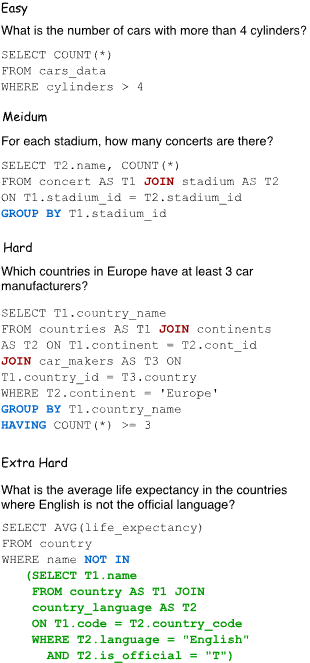
\includegraphics[width=0.35\textwidth]{image.png}
\caption{SQL query examples in 4 hardness levels. Credit: Spider (Yu et al., 2018)}
\label{fig:hardness-levels}
\end{figure}

\subsection{Prompting and Input}
\label{sec:prompting}

Each model receives three pieces of information in a single zero-shot user turn: a system instruction explaining its role as a Text-to-SQL generator, the database schema (Table names, column names, primary keys, and foreign-key relationships, with no example rows), and the natural-language question. No few-shot examples are provided, so that the experiment measures each model's ability to generate SQL from instructions and schema information alone, without the confound of examples steering its output style. The prompt template is identical across all three models, so that differences in performance can be attributed to the models rather than to differences in prompting.

\textbf{Prompt template:}
\begin{verbatim}
Given the following SQLite database schema, write a SQL query that answers
the question.

{schema}

Question: {question}

Respond with only the SQL query in a ```sql code block.
\end{verbatim}

See \hyperref[sec:appendix1]{Appendix 1} for a worked example: a full schema, a question, and the resulting filled prompt.

\subsection{SQL Extraction}
\label{sec:sql-extraction}

For each sample, we decode the model's generated tokens into text using the model-specific tokenizer, and check for the presence of a \texttt{</think>} token. If \texttt{</think>} was generated, we take all text generated before \texttt{</think>} as the reasoning trace and all text to the right as the output SQL; DeepSeek-R1-Distill-Qwen-1.5B is the only model of the three that can emit this token. The SQL is then extracted from the first \texttt{```sql} code block in that remaining text. The extracted SQL is passed to the evaluation script as-is. Outputs that cannot be extracted or parsed are counted as incorrect on every metric rather than excluded from the evaluation, as unusable output is a task failure (see \ref{sec:evaluation-metrics} and \ref{sec:invalid-outputs}).

\subsection{Inference Settings}
\label{sec:inference-settings}

All models are evaluated using the same decoding configuration: greedy decoding (temperature and top-p are not applicable) for consistent, reproducible results between runs. The maximum output length differs by model: 256 tokens for Qwen3-0.6B, and 4096 tokens for both Qwen3-4B and DeepSeek-R1-Distill-Qwen-1.5B. For DeepSeek, the larger budget is needed because its output also has to contain a full reasoning trace rather than only the SQL query; Qwen3-4B is given the same, larger budget as DeepSeek so that a tighter token limit can be ruled out as the reason for any difference between them on invalid-output rate (\ref{sec:invalid-outputs}) or inference time (\ref{sec:efficiency}). Qwen3-0.6B and Qwen3-4B are both run with thinking mode off (both support it). DeepSeek-R1-Distill-Qwen-1.5B always produces a reasoning trace and has no documented way to disable thinking mode, so it is evaluated as the reasoning condition against the two non-reasoning Qwen3 models. All inference runs on the same 1x RTX 4090 GPU described in \ref{sec:models}, with batch size 128.

\subsection{Evaluation}
\label{sec:evaluation-metrics}

We evaluate the output using the same metrics as the Spider paper (Yu et al., 2018). These are:

\begin{enumerate}
\item Component Matching
    \begin{itemize}
        \item For each of the following components:
        \begin{itemize}
            \item SELECT
            \item WHERE
            \item GROUP BY
            \item ORDER BY
            \item KEYWORDS (including all SQL keywords without column names and operators)
        \end{itemize}
        \item Decompose each component in the prediction and ground truth as bags of several sub-components and check whether or not these two sets of components match completely.
        \item Checks accuracy, recall, and F1
    \end{itemize}
\item Exact Matching Accuracy
    \begin{itemize}
        \item We measure whether the generated query as a whole is equivalent to the golden query (AKA ground truth query)
        \item The generated query is correct only if all components are correct
        \item Checks only accuracy
    \end{itemize}
\item Execution Accuracy
    \begin{itemize}
        \item A list of gold values for each question is given
        \item We measure how many gold values the generated query extracts when executed
        \item Checks only accuracy
    \end{itemize}
\end{enumerate}

If output is invalid or unparsable, then it fails exact matching and execution accuracy. Results~\ref{sec:invalid-outputs} reports how often this happens for each model.

\section{RQ1: Results}
\label{sec:rq1-results}

\subsection{Overall Model Performance}
\label{sec:overall-performance}

Below we report how Qwen3-0.6B, Qwen3-4B, and DeepSeek-R1-Distill-Qwen-1.5B perform on the Spider benchmark across all 3 metrics (Component Matching, Exact Matching Accuracy, Execution Accuracy). We calculate the values per problem difficulty as well as overall, and display them in the below tables.

\begin{table}[H]
\centering
\footnotesize
\caption{Overall performance summary, aggregated across all difficulties (all 1034 problems). Component matching is accuracy / recall / F1 (macro-averaged, see the note on Table~\ref{tab:difficulty-component} in \ref{sec:rq1-interpretation}). Per-difficulty breakdowns are in Tables~\ref{tab:difficulty-component}--\ref{tab:difficulty-execution}.}
\label{tab:overall-performance}
\resizebox{\textwidth}{!}{%
\begin{tabular}{lllccc}
\toprule
Model & Parameters & Category & Component matching & Exact matching & Execution accuracy \\
\midrule
Qwen3-0.6B & 0.6B & Decoder-only & 0.628 / 0.209 / 0.314 & 0.099 & 0.209 \\
Qwen3-4B & 4B & Decoder-only & 0.797 / 0.306 / 0.442 & 0.256 & 0.353 \\
DeepSeek-R1-Distill-Qwen-1.5B & 1.5B & Reasoning & 0.661 / 0.174 / 0.275 & 0.085 & 0.121 \\
\bottomrule
\end{tabular}}
\end{table}

All models are evaluated zero-shot with the same prompt on the 20 databases of the Spider dev set. Aggregated across all difficulties and databases, every model is still far from solving the task: execution accuracy ranges from 0.121 (DeepSeek) to 0.353 (Qwen3-4B) and exact matching accuracy from 0.085 (DeepSeek) to 0.256 (Qwen3-4B). Execution accuracy is higher than exact matching accuracy for all three models (for example 0.353 vs.\ 0.256 for Qwen3-4B), which suggests that at least some of the queries that return the correct result are written differently from the gold SQL (see Section \ref{sec:rq1-interpretation} for more on this relationship). Of the three models, Qwen3-4B is now the best on almost every metric, database, and difficulty level; Section \ref{sec:by-database} and Section \ref{sec:rq1-interpretation} quantify how consistently. Table ~\ref{tab:inference-time} reports the efficiency side of this comparison: inference time per example.

\subsection{Performance by Query Difficulty}
\label{sec:by-difficulty}

\begin{table}[H]
\centering
\footnotesize
\caption{Component matching (accuracy / recall / F1) by difficulty.}
\label{tab:difficulty-component}
\begin{tabular}{lcc}
\toprule
Model & easy & medium \\
\midrule
Problems (n) & 248 & 446 \\
Qwen3-0.6B & 0.675 / 0.308 / 0.423 & 0.582 / 0.235 / 0.334 \\
Qwen3-4B & 0.838 / 0.574 / 0.681 & 0.670 / 0.306 / 0.420 \\
DeepSeek-R1-Distill-Qwen-1.5B & 0.566 / 0.288 / 0.382 & 0.642 / 0.185 / 0.287 \\
\bottomrule
\end{tabular}

\vspace{0.5em}

\begin{tabular}{lccc}
\toprule
Model & hard & extra & all \\
\midrule
Problems (n) & 174 & 166 & 1034 \\
Qwen3-0.6B & 0.540 / 0.141 / 0.223 & 0.578 / 0.160 / 0.250 & 0.628 / 0.209 / 0.314 \\
Qwen3-4B & 0.796 / 0.262 / 0.394 & 0.485 / 0.150 / 0.229 & 0.797 / 0.306 / 0.442 \\
DeepSeek-R1-Distill-Qwen-1.5B & 0.543 / 0.113 / 0.187 & 0.389 / 0.104 / 0.164 & 0.661 / 0.174 / 0.275 \\
\bottomrule
\end{tabular}
\end{table}

\begin{table}[H]
\centering
\footnotesize
\caption{Exact matching accuracy by difficulty.}
\label{tab:difficulty-exact}
\begin{tabular}{lccccc}
\toprule
Model & easy & medium & hard & extra & all \\
\midrule
Problems (n) & 248 & 446 & 174 & 166 & 1034 \\
Qwen3-0.6B & 0.157 & 0.137 & 0.006 & 0.006 & 0.099 \\
Qwen3-4B & 0.508 & 0.262 & 0.115 & 0.012 & 0.256 \\
DeepSeek-R1-Distill-Qwen-1.5B & 0.214 & 0.078 & 0.000 & 0.000 & 0.085 \\
\bottomrule
\end{tabular}
\end{table}

\begin{table}[H]
\centering
\footnotesize
\caption{Execution accuracy by difficulty.}
\label{tab:difficulty-execution}
\begin{tabular}{lccccc}
\toprule
Model & easy & medium & hard & extra & all \\
\midrule
Problems (n) & 248 & 446 & 174 & 166 & 1034 \\
Qwen3-0.6B & 0.210 & 0.276 & 0.126 & 0.114 & 0.209 \\
Qwen3-4B & 0.565 & 0.345 & 0.276 & 0.139 & 0.353 \\
DeepSeek-R1-Distill-Qwen-1.5B & 0.258 & 0.128 & 0.017 & 0.006 & 0.121 \\
\bottomrule
\end{tabular}
\end{table}

We break every metric down by the Spider Hardness Criteria (\ref{sec:eval-data}), since aggregate numbers alone would hide whether a model's advantage holds up as queries get harder.

Performance decreases with difficulty for every model, but the decrease is steepest for Qwen3-0.6B and DeepSeek: their exact matching and execution accuracy are both at most 0.006 and 0.126 respectively on hard and extra problems, down from as high as 0.210-0.258 (easy execution) on the easiest problems (Table~\ref{tab:difficulty-exact} and Table~\ref{tab:difficulty-execution}). Qwen3-4B degrades on the same relative scale but from a much higher starting point, from 0.508 easy exact matching / 0.565 easy execution accuracy down to 0.012 extra exact matching / 0.139 extra execution accuracy. Despite the degradation, it remains the best of the three models at every single difficulty level on both metrics (Tables~\ref{tab:difficulty-exact}--\ref{tab:difficulty-execution}).

\subsection{Performance by Database}
\label{sec:by-database}

We also break execution and exact matching accuracy down by each of the 20 Spider dev databases. Qwen3-4B has the highest execution accuracy on 17 of the 20 databases outright (plus a tie on one more) and the highest exact matching accuracy on 18 of 20, while DeepSeek-R1-Distill-Qwen-1.5B is never highest on either metric; Qwen3-0.6B wins outright only on orchestra and battle\_death. Databases with few problems (real\_estate\_properties with n=4, voter\_1 with n=15, battle\_death with n=16, and museum\_visit with n=18) are too small to rank the models reliably, since a single problem changes a score by 6 to 25 percentage points. Execution accuracy ranges from 0.10 (course\_teach) to 0.53 (singer) for Qwen3-0.6B, from 0.19 (battle\_death) to 0.60 (singer) for Qwen3-4B, and from 0.00 (concert\_singer) to 0.27 (singer and voter\_1) for DeepSeek-R1-Distill-Qwen-1.5B (\hyperref[tab:db-execution]{Table 5}). 


\begin{table}[H]
\centering
\footnotesize
\caption{Execution accuracy by database (domain).}
\begin{tabular}{lcccc}
\toprule
Database & Problems (n) & Qwen3-0.6B & Qwen3-4B & DeepSeek-R1-Distill-Qwen-1.5B \\
\midrule
world\_1 & 120 & 0.183 & 0.242 & 0.108 \\
car\_1 & 92 & 0.109 & 0.315 & 0.054 \\
cre\_Doc\_Template\_Mgt & 84 & 0.202 & 0.405 & 0.071 \\
dog\_kennels & 82 & 0.159 & 0.293 & 0.085 \\
flight\_2 & 80 & 0.263 & 0.500 & 0.250 \\
student\_transcripts\_tracking & 78 & 0.128 & 0.321 & 0.064 \\
wta\_1 & 62 & 0.161 & 0.290 & 0.129 \\
tvshow & 62 & 0.339 & 0.435 & 0.129 \\
network\_1 & 56 & 0.286 & 0.375 & 0.179 \\
concert\_singer & 45 & 0.111 & 0.289 & 0.000 \\
pets\_1 & 42 & 0.167 & 0.286 & 0.071 \\
poker\_player & 40 & 0.250 & 0.550 & 0.225 \\
orchestra & 40 & 0.350 & 0.250 & 0.100 \\
employee\_hire\_evaluation & 38 & 0.105 & 0.211 & 0.132 \\
course\_teach & 30 & 0.100 & 0.500 & 0.100 \\
singer & 30 & 0.533 & 0.600 & 0.267 \\
museum\_visit & 18 & 0.278 & 0.500 & 0.222 \\
battle\_death & 16 & 0.375 & 0.188 & 0.188 \\
voter\_1 & 15 & 0.267 & 0.400 & 0.267 \\
real\_estate\_properties & 4 & 0.500 & 0.500 & 0.000 \\
\bottomrule
\label{tab:exec-acc-rq1-by-database}
\end{tabular}
\end{table}


The pattern on exact matching accuracy is just as one-sided (\hyperref[tab:db-exact]{Table 6}): Qwen3-4B is highest on 18 of 20 databases, ties Qwen3-0.6B on orchestra, and loses only on battle\_death; DeepSeek's exact matching accuracy is never the highest of the three, coming closest on flight\_2 (0.200 vs.\ Qwen3-4B's 0.350 and Qwen3-0.6B's 0.075). The full per-database tables and discussion are in \hyperref[sec:appendix2]{Appendix 2}.

\subsection{Analysis of Invalid and Unparseable Outputs}
\label{sec:invalid-outputs}

We also count how often each model's output cannot be used as SQL at all: it either never produces a usable query within the token budget (\ref{sec:inference-settings}) or is truncated before finishing one. Per \ref{sec:evaluation-metrics}, these count as failures on every metric rather than being excluded, and this is a direct measure of how reliably each model follows the ``respond with only a SQL query'' instruction, independent of whether the SQL it does produce is correct. Qwen3-0.6B's invalid rate is 2.2\%, Qwen3-4B's is 0.0\%, and DeepSeek-R1-Distill-Qwen-1.5B's is 9.7\%, about 4x higher than Qwen3-0.6B's despite having the same 4096-token budget as Qwen3-4B (\ref{sec:inference-settings}), i.e. a larger token budget did not cause Qwen3-4B to run on or produce unusable output the way it does for DeepSeek. Section \ref{sec:rq1-interpretation} breaks DeepSeek's failures down further by difficulty and by why the generation failed (see Tables~\ref{tab:deepseek-outcome}--\ref{tab:deepseek-unfinished-by-difficulty}).


\begin{table}[H]
\centering
\footnotesize
\caption{DeepSeek-R1-Distill-Qwen-1.5B by generation outcome. ``Cut'' means the generation reached the 4096-token limit.}
\label{tab:deepseek-outcome}
\begin{tabular}{lccccc}
\toprule
Outcome & Problems (n) & Share & Avg.\ tokens & Exact match & Component F1 \\
\midrule
Finished with SQL & 934 & 90.3\% & 512 & 0.094 & 0.286 \\
Finished, no usable SQL & 2 & 0.2\% & 284 & 0.000 & 0.100 \\
Cut while answering (after \texttt{</think>}) & 13 & 1.3\% & 4096 & 0.000 & 0.096 \\
Cut while thinking (no \texttt{</think>}) & 85 & 8.2\% & 4096 & 0.000 & 0.093 \\
All & 1034 & 100\% & 851 & 0.085 & 0.275 \\
\bottomrule
\end{tabular}
\end{table}

\begin{table}[H]
\centering
\footnotesize
\caption{The same 934 questions that DeepSeek finished, for all three models.}
\label{tab:deepseek-finished-934}
\begin{tabular}{lcc}
\toprule
Model & Exact match & Component F1 \\
\midrule
DeepSeek-R1-Distill-Qwen-1.5B & 0.094 & 0.286 \\
Qwen3-0.6B & 0.103 & 0.317 \\
Qwen3-4B & 0.257 & 0.440 \\
\bottomrule
\end{tabular}
\end{table}

\begin{table}[H]
\centering
\footnotesize
\caption{Share of Deepseek generations that are infinite self-repetition loops. We check self-repetition using compression ratio: a text that repeats itself compresses well, so a low compression ratio of the last 3000 characters indicates a loop. In testing, we found generations with compression ratios <0.15 infinitely self-looped.}
\label{tab:deepseek-repetition}
\begin{tabular}{lcccc}
\toprule
Generations & n & Median compression ratio & Ratio $<$ 0.15 & Last 150 characters repeat 3 or more times \\
\midrule
Cut off & 98 & 0.095 & 95.9\% & 96.9\% \\
Finished & 936 & 0.418 & 0.0\% & 0.2\% \\
\bottomrule
\end{tabular}
\end{table}

\begin{table}[H]
\centering
\footnotesize
\caption{Share of DeepSeek generations that did not finish with SQL, by difficulty.}
\label{tab:deepseek-unfinished-by-difficulty}
\begin{tabular}{lccccc}
\toprule
 & easy & medium & hard & extra & all \\
\midrule
Problems (n) & 248 & 446 & 174 & 166 & 1034 \\
Not finished with SQL (n) & 15 & 33 & 25 & 27 & 100 \\
Share & 6.0\% & 7.4\% & 14.4\% & 16.3\% & 9.7\% \\
\bottomrule
\end{tabular}
\end{table}

\subsection{Efficiency Measures}
\label{sec:efficiency}

\begin{table}[H]
\centering
\footnotesize
\caption{Output tokens per example.}
\label{tab:tokens-per-example}
\begin{tabular}{lccccc}
\toprule
Model & easy & medium & hard & extra & all \\
\midrule
Qwen3-0.6B & 27.5 & 44.7 & 53.7 & 69.9 & 46.1 \\
Qwen3-4B & 23.6 & 37.3 & 46.2 & 59.0 & 39.0 \\
DeepSeek-R1-Distill-Qwen-1.5B & 610.8 & 768.4 & 1096.0 & 1176.9 & 851.3 \\
\bottomrule
\end{tabular}
\end{table}

Inference time is measured from the start of generation to the complete batch output, per batch of 128 examples, with each batch's wall time divided evenly across its 128 examples to get the per-example figure, excluding tokenization, model loading, and warm-up.

\begin{table}[H]
\centering
\footnotesize
\caption{Inference time.}
\label{tab:inference-time}
\begin{tabular}{lcc}
\toprule
Model & Total wall time (s) & Avg.\ time per example (s) \\
\midrule
Qwen3-0.6B & 123.9 & 0.120 \\
Qwen3-4B & 109.1 & 0.106 \\
DeepSeek-R1-Distill-Qwen-1.5B & 3059.8 & 2.959 \\
\bottomrule
\end{tabular}
\end{table}

DeepSeek is about 25x slower per example than Qwen3-0.6B and 28x slower than Qwen3-4B, consistent with its much higher average token count (Table~\ref{tab:tokens-per-example}). Qwen3-4B, despite having about 7x as many parameters as Qwen3-0.6B, is marginally faster per example (0.106s vs.\ 0.120s), consistent with it generating fewer tokens on average (39.0 vs.\ 46.1, Table~\ref{tab:tokens-per-example}) despite having the same 16x larger token budget as DeepSeek (\ref{sec:inference-settings}).


\section{RQ1: Interpretation and Answer}
\label{sec:rq1-interpretation}

\textbf{RQ1:} How do (selected) LLMs perform on cross-domain Text-to-SQL?

\vspace{10px}

All three models are still far from solving the task in this zero-shot setting: exact matching accuracy ranges from 0.085 to 0.256 and execution accuracy from 0.121 to 0.353 (Table~\ref{tab:overall-performance}). Difficulty and database effects are discussed in \ref{sec:by-difficulty} and \ref{sec:by-database}; here we interpret the effects of model size and reasoning architecture and the exact-match/execution-accuracy relationship, and state the answer to RQ1 as three findings.

\subsection{First, within the Qwen family, scale is a strong and almost uniform predictor of performance, but an intermediate-size reasoning model from the DeepSeek family still loses to the smallest model in the Qwen family.}
\label{sec:rq1-finding-scale}

Aggregated across all difficulties, Qwen3-4B has the best component matching (0.797 accuracy / 0.306 recall / 0.442 F1), exact matching (0.256 ), and execution accuracy (0.353) of the three (Table~\ref{tab:overall-performance}), and it beats Qwen3-0.6B on exact matching and execution accuracy at every individual difficulty level, including hard (0.115 vs.\ 0.006) and extra (0.012 vs.\ 0.006), where the smaller model solves almost nothing (Tables~\ref{tab:difficulty-exact}--\ref{tab:difficulty-execution}). This effect is large and holds at every difficulty level. The one exception is component matching on extra-hard problems, where Qwen3-0.6B's accuracy, recall, and F1 (0.578 / 0.160 / 0.250) are all slightly higher than Qwen3-4B's (0.485 / 0.150 / 0.229), the only point in the RQ1 results where the smaller Qwen3 model wins outright (Table~\ref{tab:difficulty-component}). DeepSeek-R1-Distill-Qwen-1.5B sits between the two Qwen3 models in parameter count (1.5B) and is the only one that reasons, yet it is the lowest of the three on every aggregate metric (0.275 component F1, 0.085 exact matching, 0.121 execution accuracy) except its own component-matching accuracy (0.661 vs.\ 0.628 for Qwen3-0.6B). Thus, scale predicts performance well within a family, but does not transfer across the reasoning/non-reasoning boundary: having more parameters than Qwen3-0.6B did not help DeepSeek catch up to it.

\subsection{Second, the reasoning architecture itself, not parameter count, is the most likely driver of DeepSeek's low score.}
\label{sec:rq1-finding-reasoning}

Its invalid-output rate (9.7\%) is markedly higher than Qwen3-0.6B's (2.2\%) and Qwen3-4B's (0.0\% in this run) (\ref{sec:invalid-outputs}). In Tables~\ref{tab:deepseek-outcome}--\ref{tab:deepseek-unfinished-by-difficulty}, 100 of 1034 generations (9.7\%) end without usable SQL. 85 never leave the reasoning phase, 13 are cut while writing the answer, and 2 finish without SQL. The number of unusable SQL generations also grows with difficulty, from 6.0\% on easy to 16.3\% on extra problems. These are not cases of long productive reasoning either: 95.9\% of the cut-off generations are highly self-repetitive (compression ratio below 0.15, median compression ratio 0.095, vs.\ 0.418 for finished generations), rewriting the same query and repeating phrases like ``So the final query is:'' without converging. Finishing does not make it better either: on the 934 questions DeepSeek does finish, its exact matching (0.094) and component F1 (0.286) are still below Qwen3-0.6B's on the same questions (0.103 / 0.317) and far below Qwen3-4B's (0.257 / 0.440), despite generating 512 tokens per question on average there, against 46 and 39 tokens overall for Qwen3-0.6B and Qwen3-4B (about 11x and 13x fewer). This extra length also costs time: DeepSeek is 25-28x slower per example than either Qwen3 model (\ref{sec:efficiency}). The reasoning trace mostly lengthens the output and sometimes never terminates, without improving the SQL when it does, and size alone is not the explanation, since Qwen3-4B is both bigger than DeepSeek and the best model in the comparison. This does not fully isolate reasoning from DeepSeek's other differences from the two Qwen3 models, such as distillation (see Limitations).

\subsection{Third, query difficulty has a substantial, consistent effect on every model, including the best one.}
\label{sec:rq1-finding-difficulty}

Exact matching and execution accuracy both fall sharply from easy to extra-hard problems for all three models (\ref{sec:by-difficulty}). Qwen3-4B's drop is from a much higher base (0.508 to 0.012 exact matching, 0.565 to 0.139 execution accuracy) and it remains the best model at every difficulty level on both metrics, but the drop itself is just as steep in relative terms as for the other two models, and the hardest problems remain largely unsolved even for it.

\subsection{Exact Match vs.\ Execution Accuracy}
\label{sec:rq1-exact-vs-execution}

For all three models, execution accuracy aggregated across all difficulties exceeds exact matching accuracy (Table~\ref{tab:overall-performance}): 0.209 vs.\ 0.099 for Qwen3-0.6B, 0.353 vs.\ 0.256 for Qwen3-4B, and 0.121 vs.\ 0.085 for DeepSeek. Since exact matching requires every SQL component to match the gold query while execution accuracy only requires the same result set, this gap indicates each model writes some queries that are valid and correct but phrased differently from the gold SQL (e.g.\ a different but equivalent join order, or an explicit column list where the gold query uses \texttt{SELECT *}). The gap is widest for Qwen3-0.6B (11.0 points), close behind for Qwen3-4B (9.7 points), and narrowest for DeepSeek (3.6 points); DeepSeek's narrower gap reflects it producing fewer alternative-but-valid queries. Qwen3-4B's gap is almost as wide as Qwen3-0.6B's despite much higher absolute accuracy, so scaling up within the Qwen3 family raises both exact matching accuracy and execution accuracy together rather than closing the gap between them.

\subsection{Limitations}
\label{sec:rq1-limitations}

Our working hypothesis is that Text-to-SQL at this scale does not benefit from an explicit reasoning trace, and that a non-reasoning model is sufficient, with performance instead scaling with parameter count within a fixed model family. The results are consistent with this hypothesis. However, they do not establish that Text-to-SQL is too simple for reasoning models in general due to several factors:

\begin{itemize}
\item \textbf{Model differences beyond reasoning.} Qwen3-0.6B and Qwen3-4B share a model family, isolating the effect of scale between them, but DeepSeek differs from both in family, size, and pretraining/post-training, not only in whether it reasons; it is also a distilled model, so the effect of reasoning cannot be fully separated from distillation quality.
\item \textbf{Aggregated component matching.} The component matching figures in Table~\ref{tab:difficulty-component} (and in Table~\ref{tab:overall-performance}) are our own macro-average (mean of the 10 per-component accuracy and recall scores, with F1 computed from these two means), not a number reported by Spider.
\end{itemize}

Overall, in this zero-shot, cross-domain setting, a larger non-reasoning decoder-only model (Qwen3-4B, 4B) clearly outperforms both a same-family model at under a sixth its size (Qwen3-0.6B) and a reasoning model of intermediate size from a different family (DeepSeek-R1-Distill-Qwen-1.5B, 1.5B), while also being faster per example than either. None of the three models solve more than half of even the easiest problems or more than a small fraction of hard or extra-hard queries. This answers RQ1 for the three models evaluated. (this
% file's cross-references into Task 1 -- table~\ref{tab:deepseek-outcome},
% \ref{tab:tokens-per-example}, \ref{sec:sql-extraction}, etc. -- rely on
% RQ1.tex's labels already being defined earlier in the same document).
%
% Structure: Methodology is organized per-feature (Feature 1: Token Count,
% Feature 2: Information Retention), each with its own Definition / Why it's
% relevant / How we computed it. Results is organized as descriptive
% statistics, differences by correctness, differences by difficulty, and
% relationship with Text-to-SQL correctness (the correlation analysis).

\section{Task 2 -- RQ2: Methodology}
\label{sec:rq2-methodology}

\textbf{RQ2:} How do characteristics of reasoning traces (of reasoning LLM) relate to Text-to-SQL performance?

To answer this question, we examine two features of each reasoning trace: Token Count and Information Retention. We compute both for all 1034 generations in DeepSeek-R1-Distill-Qwen-1.5B's main Task 1 run, then relate each to difficulty and to Text-to-SQL correctness.

\subsection{Feature 1: Token Count}
\label{sec:rq2-feature-tokencount}

\textbf{Definition.} Token Count is the number of tokens in the reasoning segment of a generation, i.e.\ everything the model generates before \texttt{</think>}, excluding the final SQL answer. We split each generation into a reasoning segment and an answer segment using the same \texttt{</think>} split used in Task 1 (\ref{sec:sql-extraction}).

% We hypothesize that for each difficulty there exists a "goldilocks" token-count range, and that performance improves as the answer's token count approaches the mean of that range.

\textbf{Why it's relevant.} Examining token count allows us to investigate whether the amount of generated reasoning is associated with better Text-to-SQL performance. However, a longer trace does not necessarily mean better reasoning, since additional tokens may contain redundant or irrelevant information.

Additionally, we expect Token Count to scale positively with the difficulty of the related Text-to-SQL problem: easy questions should require fewer thinking tokens, while extra-hard questions should require significantly more. Any question that disobeys this relation, or where more tokens associate with worse rather than better answers, is given special attention in Results.

\textbf{How we computed it.} Token Count is the number of tokens in the reasoning segment only, re-tokenized with the model's own tokenizer (not the \texttt{new\_tokens} field logged during generation, which counts the whole generation, reasoning plus SQL). For generations that never emit \texttt{</think>} (truncated at the 4096-token generation limit, see Task 1's table~\ref{tab:deepseek-outcome}), the entire generated text is treated as the reasoning segment, so Token Count for these rows is effectively capped at the generation limit rather than reflecting a completed thought. This is intentional: these cases are exactly the repetition loops Task 1 identified (table~\ref{tab:deepseek-repetition}), and dropping them would hide, rather than explain, the heavy right tail in Token Count. We keep them in the Token Count analysis and flag wherever they drive a result (see finding~\ref{item:rq2-finding-tokencount-difficulty} in Results).

\begin{table}[H]
\centering
\footnotesize
\caption{Token Count: definition and computation summary.}
\label{tab:rq2-feature-tokencount-summary}
\begin{tabular}{p{0.22\textwidth}p{0.7\textwidth}}
\toprule
Property & Detail \\
\midrule
Unit & Tokens (model's own tokenizer) \\
Scope & Reasoning segment only, i.e.\ text before \texttt{</think>} \\
Range & Non-negative integer, long right tail (observed 103--4166) \\
Truncated traces & Treated as reasoning segment in full; capped at the 4096-token generation limit \\
\bottomrule
\end{tabular}
\end{table}

\subsection{Feature 2: Information Retention}
\label{sec:rq2-feature-retention}

\textbf{Definition.} Information Retention is the share of schema-shaped identifiers mentioned in a reasoning trace that actually exist as a table or column name in that question's schema. Equivalently, $$(1-\text{Information Retention})=\text{fraction of mentioned identifiers that are not grounded in the prompt}$$ or in other words, the hallucination rate of the trace.

\textbf{Why it's relevant.} We expect reasoning traces with low Information Retention (frequent hallucination of schema elements) to produce lower-performing answers than traces that stay grounded in the given schema, since inventing a table or column that doesn't exist is very likely to propagate into an incorrect query. We also expect harder problems to not cause lower Information Retention on their own; if they do, this points to the model introducing more assumptions as questions get harder, which is itself worth investigating as a bias rather than attributing the accuracy drop to difficulty alone.

\textbf{How we computed it.} We regex-extract every schema-shaped identifier the trace mentions, either quoted (e.g.\ \texttt{"Singer\_ID"}) or underscore-joined (e.g.\ \texttt{concert\_id}), and take the share of those identifiers that match a table or column name in that question's schema. An identifier that matches neither is treated as a fact the model introduced on its own, i.e., a hallucination. Traces that mention no schema identifiers at all are excluded from Information Retention (but kept for Token Count), since a 0-of-0 ratio is undefined rather than evidence of perfect or zero retention; this drops the usable sample from 1034 to 1017.

\begin{table}[H]
\centering
\footnotesize
\caption{Information Retention: definition and computation summary.}
\label{tab:rq2-feature-retention-summary}
\begin{tabular}{p{0.22\textwidth}p{0.7\textwidth}}
\toprule
Property & Detail \\
\midrule
Unit & Ratio, bounded in $[0,1]$ \\
Numerator & Schema identifiers mentioned in the trace that match a real table/column name \\
Denominator & All schema-shaped identifiers mentioned in the trace (quoted or underscore-joined) \\
Exclusions & Traces mentioning zero schema identifiers (1034 $\rightarrow$ 1017 usable rows) \\
Truncated traces & Scored over the partial text generated before truncation \\
\bottomrule
\end{tabular}
\end{table}

\subsection{Statistical approach}
\label{sec:rq2-statistical-approach}

We relate both Token Count and Information Retention to correctness and difficulty with Spearman's Rank Correlation throughout. Both of our hypotheses are about monotonic relationships, not linear relationships (performance should not decrease as Token Count or Information Retention increase, and Token Count should increase with difficulty), which is exactly what Spearman's Rank Correlation tests for. It also suits the distribution of our two reasoning metrics: Token Count is a non-negative count with a long right tail (DeepSeek alone ranges from 611 tokens on easy problems to 1177 on extra, table~\ref{tab:tokens-per-example}), and Information Retention is a bounded ratio, so neither is likely to be symmetric and unbounded; the $\geq$90\% trace completion rate gives us enough data per stratum to check this on histograms rather than assume it. For correctness, we correlate each reasoning metric against the continuous, per-question component matching accuracy, recall, and F1 for all ten Spider components individually, plus exact matching and execution accuracy.

This gives 32 submetrics per reasoning metric per difficulty level. With 169 correlation tests run in total, we correct for multiple comparisons with the Benjamini-Hochberg procedure rather than a stricter family-wise correction like Bonferroni: we are screening many related, non-independent submetrics for the strongest associations to report and discuss, not making a small number of pre-registered confirmatory claims, so controlling the expected false-discovery rate is a better fit than controlling the probability of any single false positive at the cost of statistical power.

% The Results below report Token Count and Information Retention broken down two ways: by difficulty, since that is the primary hypothesis under test, and by exact-match correctness (correct/incorrect), used for the descriptive statistics and the boxplots (figure~\ref{fig:rq2-boxplots}) because a binary split is easier to read in a table or figure than 32 continuous submetrics. The correlation analysis itself (table~\ref{tab:rq2-correlations}) still uses the continuous submetrics described above, for the statistical-power reasons given there; the binary-correctness view and the continuous-submetric view are two presentations of the same underlying data, not two different analyses.

The Results below report Token Count and Information Retention by correctness and difficulty level, with the continuous submetrics used directly in the correlation analysis (Table~\ref{tab:rq2-correlations}).


\section{RQ2: Results}
\label{sec:rq2-results}

We compute Token Count and Information Retention for all 1034 generations in DeepSeek-R1-Distill-Qwen-1.5B's main Task 1 run, and correlate each against difficulty and against all 32 per-question performance submetrics as described in the Methodology. Tables ~\ref{tab:rq2-descriptive-stats-tokencount-difficulty}, ~\ref{tab:rq2-descriptive-stats-tokencount-correctness}, ~\ref{tab:rq2-descriptive-stats-retention-difficulty}, and~\ref{tab:rq2-descriptive-stats-retention-correctness} give descriptive statistics for each feature by difficulty and by exact-match correctness; figure~\ref{fig:rq2-boxplots} shows the resulting distributions; table~\ref{tab:rq2-correlations} lists the strongest correlations.

\subsection{Descriptive statistics}
\label{sec:rq2-descriptive-stats}


\begin{table}[H]
\centering
\footnotesize
\caption{Token Count descriptive statistics, by difficulty.}
\label{tab:rq2-descriptive-stats-tokencount-difficulty}
\begin{tabular}{lcccccc}
\toprule
Group & n & mean & median & std & min & max \\
\midrule
easy & 248 & 542.3 & 329.0 & 845.2 & 103 & 4096 \\
medium & 446 & 648.2 & 374.0 & 925.7 & 191 & 4166 \\
hard & 174 & 939.2 & 425.0 & 1246.2 & 226 & 4096 \\
extra & 166 & 901.6 & 434.5 & 1199.9 & 222 & 4096 \\
\midrule
all & 1034 & 712.4 & 383.0 & 1026.2 & 103 & 4166 \\
\bottomrule
\end{tabular}
\end{table}

\begin{table}[H]
\centering
\footnotesize
\caption{Token Count descriptive statistics, by exact-match correctness (1 = exact match, 0 = not).}
\label{tab:rq2-descriptive-stats-tokencount-correctness}
\begin{tabular}{lcccccc}
\toprule
Group & n & mean & median & std & min & max \\
\midrule
exact match = 0 & 946 & 748.1 & 394.0 & 1065.6 & 103 & 4166 \\
exact match = 1 & 88 & 329.3 & 314.5 & 97.7 & 195 & 849 \\
\midrule
all & 1034 & 712.4 & 383.0 & 1026.2 & 103 & 4166 \\
\bottomrule
\end{tabular}
\end{table}

\begin{table}[H]
\centering
\footnotesize
\caption{Information Retention descriptive statistics, by difficulty. Excludes traces that mention no schema identifiers (n drops from 1034 to 1017 overall).}
\label{tab:rq2-descriptive-stats-retention-difficulty}
\begin{tabular}{lcccccc}
\toprule
Group & n & mean & median & std & min & max \\
\midrule
easy & 246 & 0.915 & 1.0 & 0.146 & 0.0 & 1.0 \\
medium & 441 & 0.905 & 1.0 & 0.148 & 0.0 & 1.0 \\
hard & 172 & 0.877 & 1.0 & 0.163 & 0.0 & 1.0 \\
extra & 158 & 0.861 & 1.0 & 0.215 & 0.0 & 1.0 \\
\midrule
all & 1017 & 0.896 & 1.0 & 0.163 & 0.0 & 1.0 \\
\bottomrule
\end{tabular}
\end{table}

\begin{table}[H]
\centering
\footnotesize
\caption{Information Retention descriptive statistics, by exact-match correctness (1 = exact match, 0 = not). Excludes traces that mention no schema identifiers (n drops from 1034 to 1017 overall).}
\label{tab:rq2-descriptive-stats-retention-correctness}
\begin{tabular}{lcccccc}
\toprule
Group & n & mean & median & std & min & max \\
\midrule
exact match = 0 & 931 & 0.893 & 1.0 & 0.166 & 0.0 & 1.0 \\
exact match = 1 & 86 & 0.924 & 1.0 & 0.123 & 0.5 & 1.0 \\
\midrule
all & 1017 & 0.896 & 1.0 & 0.163 & 0.0 & 1.0 \\
\bottomrule
\end{tabular}
\end{table}


\begin{figure}[H]
\centering
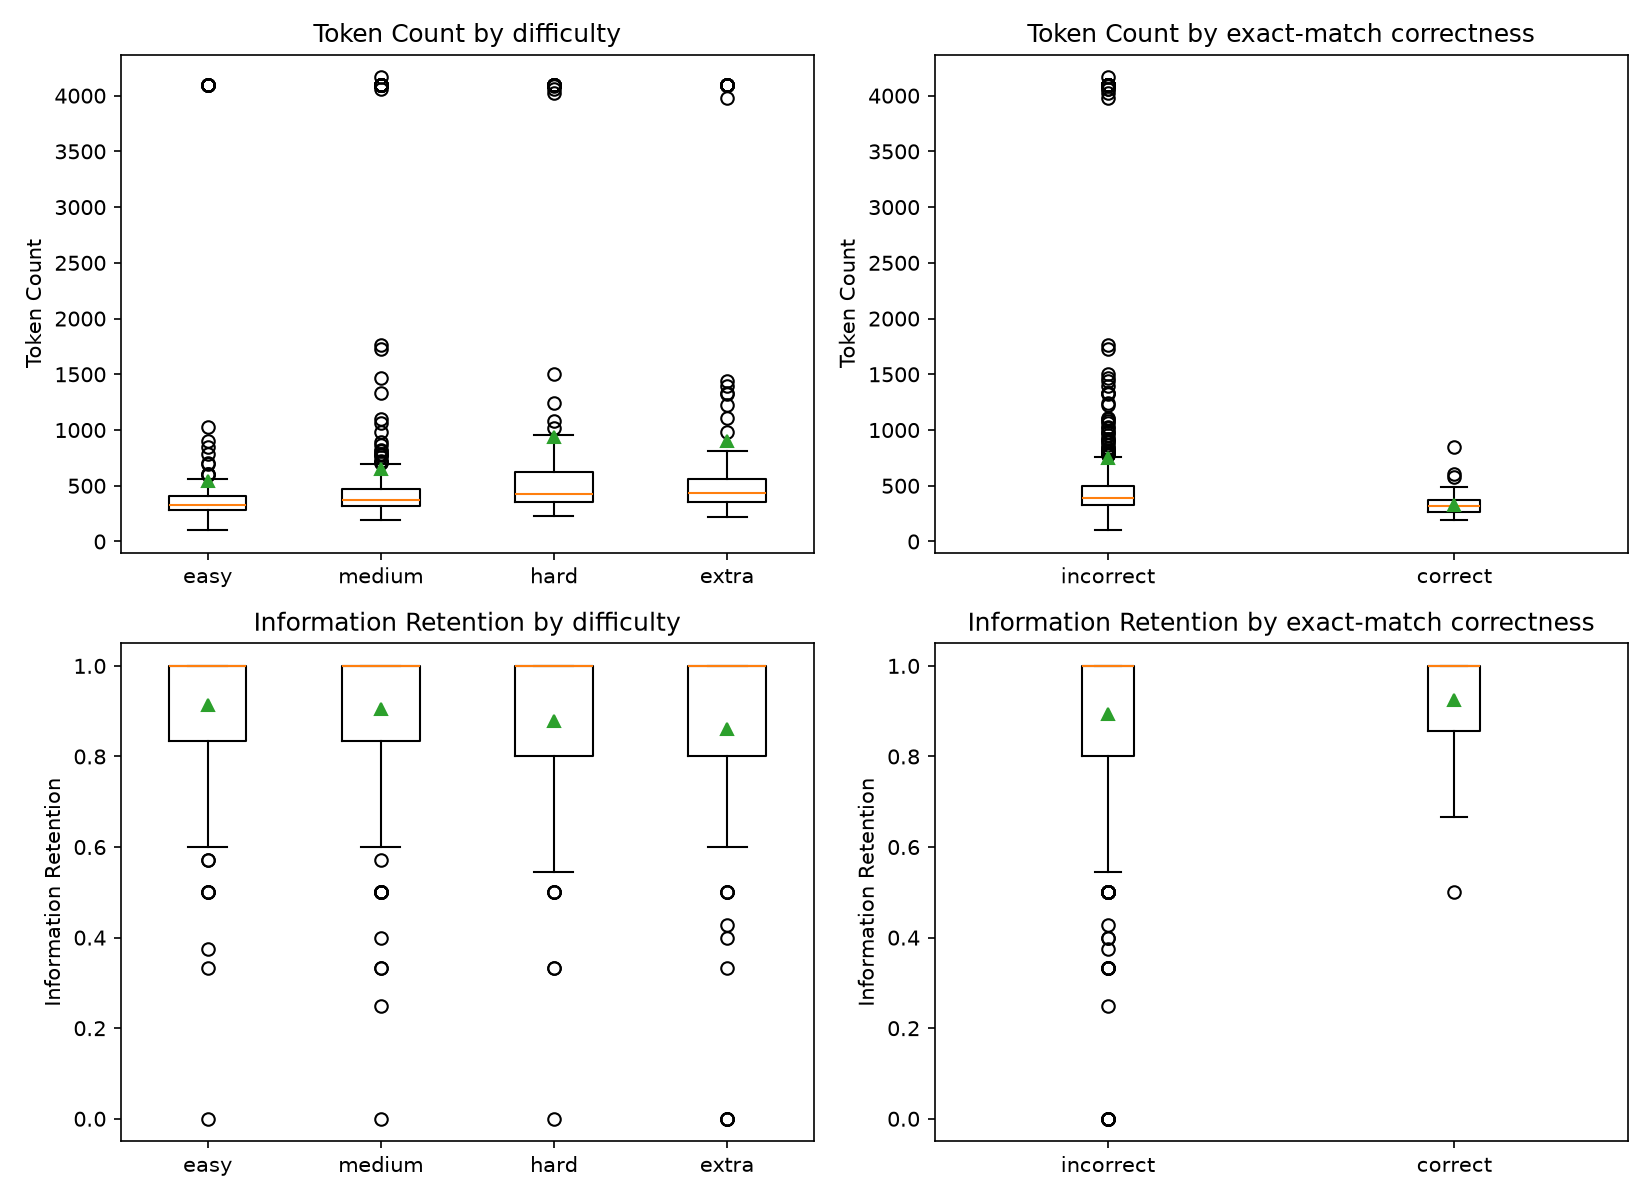
\includegraphics[width=0.85\textwidth]{boxplots.png}
\caption{Token Count and Information Retention by difficulty and by exact-match correctness, for DeepSeek-R1-Distill-Qwen-1.5B's 1034 Task 1 generations. Green triangles are means, orange lines are medians. Means sit well above medians throughout, confirming the right-skewed, bounded distributions the Methodology assumes rather than normal ones.}
\label{fig:rq2-boxplots}
\end{figure}

\subsection{Differences by correctness}
\label{sec:rq2-by-correctness}

Correct generations (exact match = 1) have a much lower mean and tighter spread of Token Count (329.3, std 97.7) than incorrect ones (748.1, std 1065.6, table~\ref{tab:rq2-descriptive-stats-tokencount-correctness}), and a slightly higher mean Information Retention (0.924 vs.\ 0.893, table~\ref{tab:rq2-descriptive-stats-retention-correctness}). Both differences point the same direction as the correlation findings in \ref{sec:rq2-relationship-correctness}: more reasoning tokens and lower retention associate with worse performance. The gap is far larger for Token Count than for Information Retention: incorrect generations' Token Count std (1065.6) is more than ten times that of correct generations (97.7), driven by the truncated, repetition-loop traces described in \ref{sec:rq2-feature-tokencount}, almost none of which are exact matches. Information Retention's median is 1.0 in both correctness groups, so the correctness gap in retention lives entirely in the mean and the lower tail, not in a shift of the typical trace. Overall, correctness tracks Token Count far more strongly than it tracks Information Retention, both in effect size and in where the gap shows up in the distribution.

\subsection{Differences by difficulty}
\label{sec:rq2-by-difficulty}

\begin{enumerate}
\item \label{item:rq2-finding-tokencount-difficulty} \textbf{Token Count increases with difficulty, as hypothesized, but the increase is driven by a heavy tail.} Median token count rises from 329 (easy) to 374 (medium) to 425 (hard) to 434 (extra), and the correlation with difficulty is positive and significant ($\rho=0.313$, $q<0.001$). The mean rises faster than the median at every level (for example 542 vs.\ 329 on easy), because generations hitting the 4096-token limit occur at every difficulty (figure~\ref{fig:rq2-boxplots}, top row); these are the same repetition loops Task 1 identified, not productive extra reasoning on harder problems.
\item \label{item:rq2-finding-retention-difficulty} \textbf{Information Retention decreases slightly with difficulty.} Median retention is 1.0 at every difficulty level, but the mean falls from 0.915 (easy) to 0.861 (extra), and the correlation with difficulty is negative and significant ($\rho=-0.107$, $q=0.013$). This is the case flagged in \ref{sec:rq2-feature-retention} as calling for closer examination of the model's introduced assumptions on harder problems.
\end{enumerate}

\subsection{Relationship with Text-to-SQL}
\label{sec:rq2-relationship-correctness}

\begin{enumerate}
\item \label{item:rq2-finding-tokencount-disobey} \textbf{On easy and medium problems, higher Token Counts track worse performance.} Token Count correlates negatively with \texttt{keywords} F1 on easy ($\rho=-0.42$, $q<0.001$) and medium ($\rho=-0.19$, $q<0.001$) problems, and with \texttt{where} and \texttt{where(no OP)} F1 on easy problems ($\rho=-0.32$ and $-0.33$, $q<0.001$). Knowing token count increases with difficulty (see ~\ref{sec:rq2-by-difficulty}), the extra tokens on these problems look like run-away generation rather than helpful deliberation.
\item \label{item:rq2-finding-retention-performance} \textbf{Where Information Retention relates to performance, it is mostly positive, as hypothesized.} On medium problems, Information Retention correlates positively with \texttt{where} and \texttt{where(no OP)} F1 ($\rho=0.345$, $q<0.001$ for both). Of its 82 submetric tests, 8 remain significant after Benjamini-Hochberg correction, 7 positive and 1 negative (\texttt{where(no OP)} recall on easy problems, $\rho=-0.261$, $q=0.042$).

\begin{table}[H]
\centering
\footnotesize
\caption{Strongest Spearman correlations between reasoning metrics and performance submetrics, Benjamini-Hochberg corrected, top 8 of 169 tests by q-value.}
\label{tab:rq2-correlations}
\begin{tabular}{llcccc}
\toprule
Metric & Submetric & Difficulty & n & $\rho$ & $q$ \\
\midrule
Token Count & difficulty (overall) & all & 1034 & 0.313 & $<$0.001 \\
Information Retention & \texttt{where} F1 & medium & 441 & 0.345 & $<$0.001 \\
Information Retention & \texttt{where(no OP)} F1 & medium & 441 & 0.345 & $<$0.001 \\
Token Count & \texttt{keywords} F1 & easy & 248 & -0.417 & $<$0.001 \\
Token Count & \texttt{where(no OP)} F1 & easy & 248 & -0.332 & $<$0.001 \\
Token Count & \texttt{where} F1 & easy & 248 & -0.322 & $<$0.001 \\
Token Count & \texttt{keywords} F1 & medium & 446 & -0.194 & $<$0.001 \\
Information Retention & difficulty (overall) & all & 1017 & -0.107 & 0.013 \\
\bottomrule
\end{tabular}
\end{table}

% \subsection{Verification: regression controlling for confounds}
% \label{sec:rq2-robustness}

% Sections~\ref{sec:rq2-by-difficulty} and~\ref{sec:rq2-relationship-correctness} test each feature against performance one at a time, but Token Count, Information Retention, and difficulty are not independent of one another: a bivariate finding there could really be driven by one of the other two variables rather than by the feature itself. The regressions below fit all three predictors jointly as statistical models, so each coefficient reflects that predictor's relationship with the outcome after the parts explained by the other two are removed, directly checking whether the findings above survive or are confounded.

% \begin{table}[H]
% \centering
% \footnotesize
% \caption{Logistic regression: exact match on standardized log Token Count, standardized Information Retention, and standardized difficulty, fit jointly ($n=1017$, pseudo $R^2=0.188$). OR is the odds ratio per one-SD increase in the predictor.}
% \label{tab:rq2-logistic}
% \begin{tabular}{lccccc}
% \toprule
% Predictor & coef & SE & $z$ & $p$ & OR [95\% CI] \\
% \midrule
% Intercept & -3.351 & 0.227 & -14.76 & $<$0.001 & 0.035 [0.022, 0.055] \\
% log Token Count ($z$) & -1.087 & 0.300 & -3.62 & $<$0.001 & 0.337 [0.187, 0.607] \\
% Information Retention ($z$) & 0.091 & 0.139 & 0.65 & 0.514 & 1.095 [0.834, 1.437] \\
% Difficulty ($z$) & -1.278 & 0.201 & -6.35 & $<$0.001 & 0.279 [0.188, 0.413] \\
% \bottomrule
% \end{tabular}
% \end{table}

% \begin{table}[H]
% \centering
% \footnotesize
% \caption{Proportional-odds (ordinal) regression: difficulty on standardized log Token Count and standardized Information Retention, fit jointly ($n=1017$). OR is the odds ratio per one-SD increase in the predictor.}
% \label{tab:rq2-ordinal}
% \begin{tabular}{lccccc}
% \toprule
% Predictor & coef & SE & $z$ & $p$ & OR [95\% CI] \\
% \midrule
% log Token Count ($z$) & 0.398 & 0.059 & 6.78 & $<$0.001 & 1.489 [1.327, 1.670] \\
% Information Retention ($z$) & -0.177 & 0.059 & -2.99 & 0.003 & 0.837 [0.746, 0.941] \\
% \bottomrule
% \end{tabular}
% \end{table}

% Controlling for the other feature and for difficulty changes which bivariate relationship survives. Token Count's association with correctness holds up: each one-SD increase in log Token Count is associated with 66\% lower odds of an exact match (OR$=0.337$, $p<0.001$), holding Information Retention and difficulty fixed (table~\ref{tab:rq2-logistic}) --- consistent with, and strengthening, finding~\ref{item:rq2-finding-tokencount-disobey}. Information Retention's association with correctness does not survive the same control (OR$=1.095$, $p=0.514$): once Token Count and difficulty are accounted for, Retention has no detectable independent effect on correctness, so the positive finding in \ref{item:rq2-finding-retention-performance} should be read as a submetric-specific, not a global, relationship. Both features' difficulty relationships, in contrast, are independent of one another: the ordinal regression finds Token Count still predicts higher difficulty (OR$=1.489$ per SD, $p<0.001$) and Information Retention still predicts lower difficulty (OR$=0.837$ per SD, $p=0.003$) when controlling for each other (table~\ref{tab:rq2-ordinal}), so neither difficulty trend in \ref{sec:rq2-by-difficulty} is simply a byproduct of the other feature's trend.

% \subsection{Regression diagnostics}
% \label{sec:rq2-diagnostics}

% The regressions in~\ref{sec:rq2-robustness} are only as trustworthy as their assumptions: if the three predictors are collinear, or if the ordinal model's proportional-odds assumption doesn't hold, the coefficients and significance levels reported there could be misleading rather than reflecting genuine independent effects. The checks below test both before those results are treated as confirmed.

% \begin{table}[H]
% \centering
% \footnotesize
% \caption{Variance inflation factors for the three predictors in the logistic regression (table~\ref{tab:rq2-logistic}).}
% \label{tab:rq2-vif}
% \begin{tabular}{lc}
% \toprule
% Predictor & VIF \\
% \midrule
% log Token Count ($z$) & 1.057 \\
% Information Retention ($z$) & 1.020 \\
% Difficulty ($z$) & 1.059 \\
% \bottomrule
% \end{tabular}
% \end{table}

% \begin{table}[H]
% \centering
% \footnotesize
% \caption{Proportional-odds check: the pooled ordinal-regression coefficient (table~\ref{tab:rq2-ordinal}) against three separately-fit cumulative-logit models, one per difficulty cutoff. Large, systematic drift across cutoffs would indicate the proportional-odds assumption does not hold.}
% \label{tab:rq2-po-check}
% \begin{tabular}{lcccc}
% \toprule
% Cutoff & coef (Token Count) & SE & coef (Retention) & SE \\
% \midrule
% pooled (proportional-odds) & 0.398 & 0.059 & -0.177 & 0.059 \\
% $P(\text{difficulty} \geq \text{medium})$ & 0.576 & 0.117 & -0.128 & 0.081 \\
% $P(\text{difficulty} \geq \text{hard})$ & 0.396 & 0.066 & -0.195 & 0.067 \\
% $P(\text{difficulty} \geq \text{extra})$ & 0.271 & 0.074 & -0.193 & 0.078 \\
% \bottomrule
% \end{tabular}
% \end{table}

% The three predictors in the logistic regression are not meaningfully collinear (all VIF $\approx 1.0$--$1.06$, well below the common rule-of-thumb threshold of 5, table~\ref{tab:rq2-vif}), so the coefficient estimates and significance levels reported in \ref{sec:rq2-robustness} are not an artifact of Token Count, Information Retention and difficulty standing in for one another. The proportional-odds check is more mixed. Information Retention's cumulative-logit coefficient is stable across all three cutoffs ($-0.128$, $-0.195$, $-0.193$, table~\ref{tab:rq2-po-check}), consistent with the pooled $-0.177$ and with the proportional-odds assumption holding for this feature. Token Count's coefficient, however, declines monotonically across cutoffs (0.576 at the easy/medium boundary, down to 0.271 at the hard/extra boundary): Token Count distinguishes difficulty levels well at the low end but loses discriminative power at the high end, a mild violation of the proportional-odds assumption that the single pooled coefficient in table~\ref{tab:rq2-ordinal} averages over. This does not overturn the ordinal regression's conclusion that Token Count predicts difficulty (every individual cutoff coefficient is still positive and more than 3 standard errors from zero), but it means the pooled OR$=1.489$ should be read as an average effect across difficulty levels rather than a uniform one.

\section{Task 3 -- RQ3: Methodology}
\label{sec:rq3-methodology}

\textbf{RQ3:} To what extent does PlanPlay-SQL improve Qwen3-0.6B?

\subsection{Model and Option Selection}
\label{sec:rq3-model-selection}

\textbf{We select Option B -- Adaptation / Learning to Adapt: we adapt Qwen3-0.6B's parameters using PlanPlay-SQL}, rather than Option A's reasoning-only strategies. Text-to-SQL requires substantial schema understanding, and precise SQl generaiton. This makes Qwen3-0.6B an interesting model to improve, as its relatively small size makes it computationally efficient and accessible for fine-tuning.

\subsection{Approach: PlanPlay-SQL in Four Stages}
\label{sec:rq3-approach}

We call our method \textbf{PlanPlay-SQL}: the model first writes a short \emph{plan}, then is trained by verified self-\emph{play}. It combines three ideas from recent work on small-model Text-to-SQL into four stages, each motivated by a specific gap in the base model:

\begin{enumerate}
\item \textbf{Plan prompting.} From Enhancing LLM Fine-Tuning for Text-to-SQLs (2024) and FINER-SQL (2026), the model writes a short plan (tables and joins, columns, filters, aggregation and ordering) before the SQL. \emph{Why:} a model with no thinking mode otherwise has no scratch space to organize the schema before committing to SQL syntax.
\item \textbf{Supervised warm start}: we attach a fresh LoRA adapter to the frozen base checkpoint and train only the adapter to imitate the gold SQL and its rule-based plan. \emph{Why:} Task 1 showed many of the model's outputs are valid SQL that differs from the gold query, so the fastest way to close that gap is to show it Spider's own conventions directly.
\item \textbf{Verification-based iterative fine-tuning (VBI-FT)}, following SPFT-SQL (2025): the model answers training questions, we execute its SQL and the gold SQL, keep the answers with matching results as positives, and fine-tune on them. \emph{Why:} this trains on the model's own output distribution rather than only gold text, which should reduce remaining execution errors without needing additional human-labeled data.
\item \textbf{Self-play fine-tuning}, using the logistic loss of SPIN (Chen et al., 2024): we train the best checkpoint to prefer the gold answer over an incorrect answer produced by the worst checkpoint. \emph{Why:} SPFT-SQL (2025) found this stage added a further 0.6 to 0.8 points on top of verification-based fine-tuning, on much larger models, so we test whether a comparable gain appears at 0.6B.
\end{enumerate}

We train using Spider's provided training split, and checkpoints are selected on held-out training databases (\ref{sec:rq3-evaluation}), so the dev set stays untouched and evaluation stays cross-domain. We skip SPFT-SQL's (2025) synthetic question generation because Spider already provides gold SQL to execute against.

We expect PlanPlay-SQL to improve performance in several ways: stage 1 (the plan prompt with no fine-tuning) serves as a control that isolates what the prompt format contributes on its own, so any further gain from stage 2 onward can be attributed to training the model to use the format rather than to the format itself. Stage 2 (the warm start) should raise exact and execution accuracy most, since it directly targets the style gap identified in \ref{sec:rq3-model-selection}. Stage 3 (verification-based fine-tuning) then trains on the model's own execution-verified outputs rather than only gold text, which should reduce its remaining execution errors without needing additional gold-labeled data. Stage 4 (self-play) should add a further small gain on top of stage 3, by analogy with SPFT-SQL's (2025) 0.6-to-0.8-point gain on larger models. To measure each part, we report five rows on the same dev set and metrics as \hyperref[sec:rq1-results]{Task 1}: the original solution, the plan prompt only, the warm start only, warm start plus verification fine-tuning, and the full PlanPlay-SQL.



\subsection{Model Training}
\label{sec:rq3-training}

Spider's Gold SQL has no plan annotation, so we use a rule-based parser to generate stage 2's warm-start target. The parser reads each gold query's top-level clauses (FROM/JOIN, SELECT, WHERE, GROUP BY/ORDER BY/LIMIT, and any set operator) with a small regex-based SQL splitter and deterministically renders them into the five-line plan format used as the training target.

All stages use LoRA adapters (rank 32, alpha 64) on top of the frozen base checkpoint, rather than full fine-tuning, as LoRA fine-tuning achieves identical performance as full fine-tuning for most tasks at significantly less compute, memory, and storage cost.

Table~\ref{tab:rq3-training-settings} gives the learning rate, epochs, batch size, and training-item counts actually used for each stage; all stages share seed 0 and the same 707-question, 20-database held-out validation set described in \ref{sec:rq3-evaluation}. ``Samples per question'' (k) is the number of candidate SQL completions per training question sampled at temperature 0.7 and top-p 0.95 during verification-based and self-play fine-tuning (stages 3-4), before the correctness filter is applied; the resulting training-item count after filtering is reported in the ``training items'' column, since not every sampled question yields a usable positive or preference pair. Self-play additionally requires a second, frozen \emph{opponent} checkpoint: the opponent is sampled to supply the incorrect half of each preference pair, and the loss measures the trained (``policy'') checkpoint's margin between the correct and incorrect completions relative to the opponent's own margin on the same pair. Rows A-C (plain supervised or verification-based fine-tuning) have no opponent, since they have no preference pair at all. Row D is labeled as step 1 of the lower-LR self-play branch, but the step itself is a plain VBI-FT pass on a separate 800-question sample, used only to produce a slightly improved policy checkpoint for row E; it likewise has no opponent. Rows E and F are the only two rows that actually run the self-play preference-loss step.

\begin{table}[H]
\centering
\footnotesize
\caption{Training settings for each stage. Learning rate is the peak LR under a linear schedule. ``---'' marks columns that do not apply to a given row (no opponent checkpoint for non-self-play stages; no sampling for gold-only stages).}
\label{tab:rq3-training-settings}
\resizebox{\textwidth}{!}{%
\begin{tabular}{llllccccc}
\toprule
Stage & Policy init & Opponent & Training items & \# of Samples per Training Question & LR & Epochs & Batch & Rounds \\
\midrule
A: Warm start (plan format, 1500 gold) & Qwen3-0.6B & --- & 1500 gold SQL+plan pairs & --- & 2e-4 & 3 & 32 & 1 \\
B: A + 1500 further gold (supervised control) & Warm start & --- & 1500 gold SQL+plan pairs & --- & 1e-4 & 1 & 32 & 1 \\
C: B + VBI-FT (1500 q, hard only) & Warm start & --- & 476 verified positives (of 1500 sampled) & 4 & 1e-4 & 1 & 32 & 1 \\
D: self-play (lower LR), step 1/2: internal VBI-FT (own 800 q) & Warm start & --- & 946 verified positives (of 800 sampled) & 4 & 5e-5 & 1 & 32 & 1 of 2 planned \\
E: self-play (lower LR), step 2/2: preference training & D's checkpoint (val.\ acc.\ 0.624) & Warm start & 279 verified preference pairs (of 800 sampled) & 4 & 1e-5 & 1 & 32 & 1 of 2 planned \\
F: self-play (higher LR), round 1 & Warm start & Warm start (same checkpoint; round 1 has no earlier opponent) & 727 verified preference pairs (of 1500 sampled) & 4 & 1e-4 & 2 & 32 & 1 \\
\bottomrule
\end{tabular}}
\end{table}

\subsection{Evaluation Setup}
\label{sec:rq3-evaluation}

See \hyperref[sec:appendix4]{Appendix 4} for the full PlanPlay-SQL prompt template and the rule-based parser that renders gold SQL into the plan format used as the warm-start training target.

We evaluate on the same 1034-question Spider dev set and the same metrics as \hyperref[sec:rq1-results]{Task 1} (component matching, exact matching, execution accuracy), so that Task 3's comparison is a direct extension of Task 1 rather than a new benchmark. The adapted model uses the PlanPlay-SQL prompt, greedy decoding, and a maximum of 384 new tokens (Task 1: 256).

Checkpoints across all stages are selected on a held-out validation set of 707 questions from 20 training databases that were never used for training, keeping the dev set untouched for a single final comparison as well as keeping evaluation cross-domain. This mimics how the Spider benchmark was used in Task 1.

\section{RQ3: Results}
\label{sec:rq3-results}

\subsection{Overall Results}
\label{sec:rq3-results-overall}

Table~\ref{tab:rq3-dev-results-06b} compares the original Qwen3-0.6B from \hyperref[sec:rq1-results]{Task 1} with the PlanPlay-SQL-adapted model on the same 1034 Spider dev questions, with the same metrics and the same execution-checking databases.

\begin{table}[H]
\centering
\footnotesize
\caption{Original and adapted Qwen3-0.6B on the Spider dev set, overall and by difficulty. Component matching is accuracy / recall / F1 (macro-averaged as in \hyperref[sec:rq1-interpretation]{Task 1}). Execution accuracy is on mock databases.}
\label{tab:rq3-dev-results-06b}
\resizebox{\textwidth}{!}{%
\begin{tabular}{llccccc}
\toprule
Metric & Model & easy & medium & hard & extra & all \\
\midrule
Problems (n) & & 248 & 446 & 174 & 166 & 1034 \\
Component matching & Original (Task 1) & 0.675 / 0.308 / 0.423 & 0.582 / 0.235 / 0.334 & 0.540 / 0.141 / 0.223 & 0.578 / 0.160 / 0.250 & 0.628 / 0.209 / 0.314 \\
 & Adapted & 0.809 / 0.763 / 0.786 & 0.750 / 0.643 / 0.693 & 0.815 / 0.626 / 0.708 & 0.696 / 0.478 / 0.567 & 0.783 / 0.636 / 0.702 \\
Exact matching & Original (Task 1) & 0.157 & 0.137 & 0.006 & 0.006 & 0.099 \\
 & Adapted & 0.762 & 0.594 & 0.385 & 0.265 & 0.546 \\
Execution (mock DB) & Original (Task 1) & 0.173 & 0.179 & 0.029 & 0.036 & 0.130 \\
 & Adapted & 0.794 & 0.583 & 0.443 & 0.277 & 0.561 \\
\bottomrule
\end{tabular}}
\end{table}

The adapted model is better than the original on every metric and every difficulty level. Exact matching accuracy rises from 0.099 to 0.546 overall, execution accuracy on the mock databases rises from 0.130 to 0.561, and component matching recall rises from 0.209 to 0.636, so the model now writes most of the components the gold query contains. Our motivating claim in \ref{sec:rq3-model-selection} (adapting Qwen3-0.6B's parameters (Option B) on the Spider training split would close its style gap) held, with much larger gains than we expected from a 0.6B model.

\subsection{Results by Difficulty Level}
\label{sec:rq3-results-difficulty}

The gain is not uniform across difficulty. The largest relative gains are on hard (exact matching 0.006 to 0.385) and extra (0.006 to 0.265) problems, which the original model almost never solved. This is consistent with the warm start fixing a systematic style/convention gap rather than a difficulty-specific one, since harder questions have the most schema and clause structure for the plan format to organize. Easy and medium problems also improve substantially (exact matching 0.157 to 0.762 and 0.137 to 0.594 respectively), so the adaptation is not merely redistributing accuracy toward harder cases at the expense of easy ones.

\subsection{Metrics Breakdown}
\label{sec:rq3-metrics-breakdown}

The three metrics agree on direction but differ in what they reveal. Execution accuracy (0.130 to 0.561) and exact matching (0.099 to 0.546) rise by nearly the same amount, so the model is not merely producing lucky executions on the mock databases but genuinely matching gold queries. Component matching recall rises further in relative terms (0.209 to 0.636), meaning the model now includes most gold-query components even in cases where it falls short of an exact or executable match (see Table~\ref{tab:rq3-component-breakdown-06b})

\begin{table}[H]
\centering
\footnotesize
\caption{Component Matching accuracy by SQL component, original vs.\ PlanPlay-SQL-adapted Qwen3-0.6B, on the same 1034 Spider dev questions as table~\ref{tab:rq3-dev-results-06b}. Component-matching accuracy does not depend on the execution databases.}
\label{tab:rq3-component-breakdown-06b}
\resizebox{0.7\textwidth}{!}{%
\begin{tabular}{llccccc}
\toprule
Component & Model & easy & medium & hard & extra & all \\
\midrule
select & Original & 0.844 & 0.819 & 0.960 & 0.862 & 0.843 \\
 & Adapted & 0.956 & 0.855 & 0.975 & 0.792 & 0.892 \\
select (no AGG) & Original & 0.875 & 0.839 & 0.960 & 0.862 & 0.861 \\
 & Adapted & 0.973 & 0.866 & 0.975 & 0.792 & 0.901 \\
where & Original & 0.711 & 0.359 & 0.150 & 0.158 & 0.391 \\
 & Adapted & 0.875 & 0.833 & 0.694 & 0.569 & 0.784 \\
where (no OP) & Original & 0.711 & 0.391 & 0.200 & 0.368 & 0.438 \\
 & Adapted & 0.896 & 0.833 & 0.726 & 0.667 & 0.808 \\
group (no Having) & Original & 1.000 & 0.667 & 1.000 & 1.000 & 0.900 \\
 & Adapted & 0.850 & 0.741 & 0.857 & 0.696 & 0.758 \\
group & Original & 0.000 & 0.667 & 1.000 & 1.000 & 0.800 \\
 & Adapted & 0.750 & 0.672 & 0.857 & 0.625 & 0.696 \\
order & Original & 0.810 & 0.571 & 0.000 & 0.333 & 0.552 \\
 & Adapted & 0.864 & 0.833 & 0.900 & 0.875 & 0.866 \\
and/or & Original & 1.000 & 0.916 & 0.893 & 0.883 & 0.927 \\
 & Adapted & 1.000 & 0.966 & 0.959 & 0.905 & 0.964 \\
IUEN & Original & 0.000 & 0.000 & 0.000 & 0.000 & 0.000 \\
 & Adapted & 0.000 & 0.000 & 0.400 & 0.231 & 0.288 \\
keywords & Original & 0.800 & 0.591 & 0.240 & 0.310 & 0.572 \\
 & Adapted & 0.928 & 0.906 & 0.803 & 0.811 & 0.878 \\
\bottomrule
\end{tabular}}
\end{table}

\subsection{Stage-wise Ablation}
\label{sec:rq3-ablation}

To see which part of the method helps, table~\ref{tab:rq3-validation-accuracy-06b} reports accuracy on the held-out validation set of 707 questions after each stage. The rows correspond to table~\ref{tab:rq3-training-settings} as follows (counting table~\ref{tab:rq3-validation-accuracy-06b}'s first data row, ``Base model, original prompt*,'' as row 1): the warm start row 3, the supervised control is row 4, VBI-FT is row 5, the combined lower-LR self-play branch is row 6, and the higher-LR self-play branch is row 7.

\begin{table}[H]
\centering
\footnotesize
\caption{Validation accuracy (execution match on mock databases, 707 questions) after each stage. The row marked * uses a 300-question subset of the same validation set.}
\label{tab:rq3-validation-accuracy-06b}
\begin{tabular}{lc}
\toprule
Stage & Validation accuracy \\
\midrule
1. Base model, original prompt* & 0.407 \\
2. Base model, plan prompt, no training* & 0.050 \\
3. Warm start on 1500 gold questions (plan format) & 0.622 \\
4. + 1500 further gold questions (supervised control) & 0.652 \\
5. + VBI-FT on the same 1500 questions (no gold SQL, hard questions only, 476 verified samples) & 0.651 \\
6. + self-play, lower learning rate (1e-5, 9 steps) & 0.631 \\
7. + self-play, higher learning rate (1e-4, 46 steps) & 0.034 \\
\bottomrule
\end{tabular}
\end{table}

Stage 1's premise did not hold: giving the base model the plan-prompt format with no fine-tuning does not add scratch space for it to organize the schema, as \ref{sec:rq3-approach} motivated it. Instead, it collapses validation accuracy from 0.407 to 0.050, a far larger effect than a neutral control would produce. A model never trained on the plan format has no reason to follow it, so it most likely spends the budget on a malformed or incomplete plan instead of SQL, rather than using the extra structure productively. 

However, the warm start recovers from this collapse and accounts for most of the overall gain (0.050 to 0.622, or 0.407 to 0.622 against the better zero-shot baseline). Verification-based fine-tuning (stage 3) matched the supervised control (0.651 vs.\ 0.652, a difference far smaller than the roughly 2-point sampling error of 707 questions) while using only 476 self-generated, execution-verified training items instead of 1500 gold ones and no gold SQL text. This shows the model can close most of its remaining gap on its own verified outputs using LoRA fine-tuning and VBI-FT.


Our expectation that stage 4 would add a further, smaller gain as in SPFT-SQL (2025) did not hold. Self-play did not help: with a low learning rate it barely changed the model (0.622 to 0.631), and with a higher learning rate the training loss fell from 0.69 to 0.25 but accuracy collapsed to 0.034 with most outputs failing to execute. This is more pronounced than SPFT-SQL's (2025) own small gains on much larger models: self-play's margin at 0.6B is thin enough that a higher learning rate overshoots it entirely. We did not rerun the higher-learning-rate setting with intermediate checkpointing or a lower learning rate, so we cannot rule out that a different schedule would recover some of the gain the lower-LR run showed.

\subsection{Examples}
\label{sec:rq3-examples}

Out of 1034 dev questions, the adapted model gets 474 right that the original got wrong, loses 28 that the original got right, and both get 106 right (execution match on mock databases). One fixed example is the network\_1 question ``Show the student IDs and numbers of friends corresponding to each.'' The original model wrote \texttt{SELECT h.ID, h.name, h.grade, f.friend\_id FROM Highschooler h JOIN Friend f ON h.ID = f.student\_id}, which lists friends instead of counting them. The adapted model first wrote the plan \texttt{tables: friend; select: student\_id , count(*); group/order: group by student\_id} and then \texttt{SELECT student\_id , count(*) FROM friend GROUP BY student\_id}, which matches the gold query. One broken example is the tvshow question ``What are the titles of the cartoons sorted alphabetically?'' The original model wrote a correct query (\texttt{SELECT Title FROM Cartoon ORDER BY Title ASC}), but the adapted model's plan misspelled the table name (\texttt{tables: CARTON}), and the SQL that followed inherited the error (\texttt{SELECT Title FROM CARTON ORDER BY Title}), which fails to run. In this case the plan step propagated a mistake into the final query.

\subsection{Limitations}
\label{sec:rq3-limitations}

\begin{itemize}
\item \textbf{Mock databases.} The official Spider database files with rows were not available, so we generated databases with random rows seeded from the literals in each question's gold query. Execution accuracy on them only approximates the official execution accuracy. For example, Task 1's execution accuracy for the original model drops from 0.209 on schema-only databases to 0.130 on the mock databases (table~\ref{tab:overall-performance}), because on empty databases every query that returns nothing counts as "correct". Exact matching accuracy does not depend on the databases.
\item \textbf{Different prompt and token budget.} The adapted model uses a different prompt and a larger token budget than the original, so the gain combines fine-tuning, the plan format, and the longer limit.
\end{itemize}


\section*{Task 4:}

Generative AI tools were used in this assignment in a supporting capacity, with all substantive judgment and final work remaining my own. Claude was used to architect the scaffolding for the experiment runners and the Jupyter notebook, and I verified this code by running it, sampling its outputs, and manually checking them for correctness. I frequently had to fill in what the AI left incomplete, such as managing GPU memory and compute at runtime, and to correct experiment setup scripts that were set up incorrectly. I manually reviewed all output data and results and handwrote the first draft of the report myself. I then improved the report over several iterations, combining my own judgment with feedback from ChatGPT review agents.

\section*{References}

\begin{enumerate}[leftmargin=2.2em, label={[\arabic*]}]
\item Tao Yu, Rui Zhang, Kai Yang, Michihiro Yasunaga, Dongxu Wang, Zifan Li, James Ma, Irene Li, Qingning Yao, Shanelle Roman, Zilin Zhang, and Dragomir Radev. 2018. Spider: A Large-Scale Human-Labeled Dataset for Complex and Cross-Domain Semantic Parsing and Text-to-SQL Task. In Proceedings of the 2018 Conference on Empirical Methods in Natural Language Processing (EMNLP), pages 3911-3921, Brussels, Belgium. \url{https://aclanthology.org/D18-1425/} (arXiv:1809.08887)
\setcounter{enumi}{1}
\item Qwen Team. 2025. Qwen3 Technical Report. arXiv:2505.09388. \url{https://arxiv.org/abs/2505.09388}
\setcounter{enumi}{3}
\item DeepSeek-AI. 2025. DeepSeek-R1: Incentivizing Reasoning Capability in LLMs via Reinforcement Learning. arXiv:2501.12948. \url{https://arxiv.org/abs/2501.12948}
\item SPFT-SQL: Enhancing Large Language Model for Text-to-SQL Parsing by Self-Play Fine-Tuning. 2025. arXiv:2509.03937. \url{https://arxiv.org/abs/2509.03937}
\item FINER-SQL: Boosting Small Language Models for Text-to-SQL. 2026. arXiv:2605.03465. \url{https://arxiv.org/abs/2605.03465}
\item Enhancing LLM Fine-tuning for Text-to-SQLs by SQL Quality Measurement. 2024. arXiv:2410.01869. \url{https://arxiv.org/abs/2410.01869} [todo: add authors for [5]-[7]]
\item Zixiang Chen, Yihe Deng, Huizhuo Yuan, Kaixuan Ji, and Quanquan Gu. 2024. Self-Play Fine-Tuning Converts Weak Language Models to Strong Language Models. arXiv:2401.01335. \url{https://arxiv.org/abs/2401.01335} [todo: verify authors and ID]
\end{enumerate}

\section*{Appendix 1: Worked Prompt Example (Task 1)}

Referenced from 1.3 Prompting and Input Representation. One of the schemas used is:

\begin{verbatim}
CREATE TABLE "stadium" (
  "Stadium_ID" NUMERIC, "Location" TEXT, "Name" TEXT, "Capacity" NUMERIC,
  "Highest" NUMERIC, "Lowest" NUMERIC, "Average" NUMERIC,
  PRIMARY KEY ("Stadium_ID")
)

CREATE TABLE "singer" (
  "Singer_ID" NUMERIC, "Name" TEXT, "Country" TEXT, "Song_Name" TEXT,
  "Song_release_year" TEXT, "Age" NUMERIC, "Is_male" TEXT,
  PRIMARY KEY ("Singer_ID")
)

CREATE TABLE "concert" (
  "concert_ID" NUMERIC, "concert_Name" TEXT, "Theme" TEXT, "Stadium_ID" TEXT, "Year" TEXT,
  PRIMARY KEY ("concert_ID"),
  FOREIGN KEY ("Stadium_ID") REFERENCES "stadium"("Stadium_ID")
)

CREATE TABLE "singer_in_concert" (
  "concert_ID" NUMERIC, "Singer_ID" TEXT,
  PRIMARY KEY ("concert_ID"),
  FOREIGN KEY ("concert_ID") REFERENCES "concert"("concert_ID"),
  FOREIGN KEY ("Singer_ID") REFERENCES "singer"("Singer_ID")
)
\end{verbatim}

we could ask the question:
\begin{verbatim}
How many singers do we have?
\end{verbatim}

to form a prompt like:

\begin{verbatim}
Given the following SQLite database schema, write a SQL query that answers
the question.

CREATE TABLE "stadium" (
  "Stadium_ID" NUMERIC, "Location" TEXT, "Name" TEXT, "Capacity" NUMERIC,
  "Highest" NUMERIC, "Lowest" NUMERIC, "Average" NUMERIC,
  PRIMARY KEY ("Stadium_ID")
)

CREATE TABLE "singer" (
  "Singer_ID" NUMERIC, "Name" TEXT, "Country" TEXT, "Song_Name" TEXT,
  "Song_release_year" TEXT, "Age" NUMERIC, "Is_male" TEXT,
  PRIMARY KEY ("Singer_ID")
)

CREATE TABLE "concert" (
  "concert_ID" NUMERIC, "concert_Name" TEXT, "Theme" TEXT, "Stadium_ID" TEXT, "Year" TEXT,
  PRIMARY KEY ("concert_ID"),
  FOREIGN KEY ("Stadium_ID") REFERENCES "stadium"("Stadium_ID")
)

CREATE TABLE "singer_in_concert" (
  "concert_ID" NUMERIC, "Singer_ID" TEXT,
  PRIMARY KEY ("concert_ID"),
  FOREIGN KEY ("concert_ID") REFERENCES "concert"("concert_ID"),
  FOREIGN KEY ("Singer_ID") REFERENCES "singer"("Singer_ID")
)

Question: How many singers do we have?

Respond with only the SQL query in a ```sql code block.
\end{verbatim}

\section*{Appendix 2: Performance by Database (Task 1)}

Referenced from 2.3 Performance by Database. Tables 5 and 6 report execution and exact matching accuracy on each of the 20 Spider dev databases, all of which are unseen by the models.

\begin{table}[H]
\centering
\footnotesize
\caption{Table 5: Execution accuracy by database (domain).}
\begin{tabular}{lcccc}
\toprule
Database & Problems (n) & Qwen3-0.6B & Qwen3-4B & DeepSeek-R1-Distill-Qwen-1.5B \\
\midrule
world\_1 & 120 & 0.183 & 0.242 & 0.108 \\
car\_1 & 92 & 0.109 & 0.315 & 0.054 \\
cre\_Doc\_Template\_Mgt & 84 & 0.202 & 0.405 & 0.071 \\
dog\_kennels & 82 & 0.159 & 0.293 & 0.085 \\
flight\_2 & 80 & 0.263 & 0.500 & 0.250 \\
student\_transcripts\_tracking & 78 & 0.128 & 0.321 & 0.064 \\
wta\_1 & 62 & 0.161 & 0.290 & 0.129 \\
tvshow & 62 & 0.339 & 0.435 & 0.129 \\
network\_1 & 56 & 0.286 & 0.375 & 0.179 \\
concert\_singer & 45 & 0.111 & 0.289 & 0.000 \\
pets\_1 & 42 & 0.167 & 0.286 & 0.071 \\
poker\_player & 40 & 0.250 & 0.550 & 0.225 \\
orchestra & 40 & 0.350 & 0.250 & 0.100 \\
employee\_hire\_evaluation & 38 & 0.105 & 0.211 & 0.132 \\
course\_teach & 30 & 0.100 & 0.500 & 0.100 \\
singer & 30 & 0.533 & 0.600 & 0.267 \\
museum\_visit & 18 & 0.278 & 0.500 & 0.222 \\
battle\_death & 16 & 0.375 & 0.188 & 0.188 \\
voter\_1 & 15 & 0.267 & 0.400 & 0.267 \\
real\_estate\_properties & 4 & 0.500 & 0.500 & 0.000 \\
\bottomrule
\end{tabular}
\end{table}

\begin{table}[H]
\centering
\footnotesize
\caption{Table 6: Exact matching accuracy by database (domain).}
\begin{tabular}{lcccc}
\toprule
Database & Problems (n) & Qwen3-0.6B & Qwen3-4B & DeepSeek-R1-Distill-Qwen-1.5B \\
\midrule
world\_1 & 120 & 0.067 & 0.142 & 0.025 \\
car\_1 & 92 & 0.043 & 0.152 & 0.033 \\
cre\_Doc\_Template\_Mgt & 84 & 0.071 & 0.238 & 0.071 \\
dog\_kennels & 82 & 0.085 & 0.244 & 0.061 \\
flight\_2 & 80 & 0.075 & 0.350 & 0.200 \\
student\_transcripts\_tracking & 78 & 0.090 & 0.269 & 0.064 \\
wta\_1 & 62 & 0.065 & 0.177 & 0.129 \\
tvshow & 62 & 0.226 & 0.339 & 0.097 \\
network\_1 & 56 & 0.125 & 0.214 & 0.179 \\
concert\_singer & 45 & 0.022 & 0.178 & 0.000 \\
pets\_1 & 42 & 0.000 & 0.095 & 0.024 \\
poker\_player & 40 & 0.175 & 0.550 & 0.100 \\
orchestra & 40 & 0.225 & 0.225 & 0.100 \\
employee\_hire\_evaluation & 38 & 0.105 & 0.158 & 0.105 \\
course\_teach & 30 & 0.033 & 0.500 & 0.067 \\
singer & 30 & 0.333 & 0.600 & 0.167 \\
museum\_visit & 18 & 0.056 & 0.500 & 0.111 \\
battle\_death & 16 & 0.250 & 0.188 & 0.062 \\
voter\_1 & 15 & 0.133 & 0.400 & 0.200 \\
real\_estate\_properties & 4 & 0.000 & 0.250 & 0.000 \\
\bottomrule
\end{tabular}
\end{table}

Execution accuracy ranges from 0.10 (course\_teach) to 0.53 (singer) for Qwen3-0.6B, from 0.19 (battle\_death) to 0.60 (singer) for Qwen3-4B, and from 0.00 (concert\_singer) to 0.27 (singer and voter\_1) for DeepSeek-R1-Distill-Qwen-1.5B. One model now wins or ties almost everywhere: Qwen3-4B has the highest execution accuracy on 17 of the 20 databases outright and ties for highest on a further 1 (real\_estate\_properties, n=4), Qwen3-0.6B is highest on the remaining 2 (orchestra and battle\_death), and DeepSeek-R1-Distill-Qwen-1.5B is highest on none. The pattern on exact matching accuracy (table 6) is just as one-sided: Qwen3-4B is highest on 18 of 20 databases, ties Qwen3-0.6B on orchestra, and loses only on battle\_death; DeepSeek's exact matching accuracy is never the highest of the three, including on flight\_2, where it comes closest (0.200 vs.\ Qwen3-4B's 0.350 and Qwen3-0.6B's 0.075). Databases with few problems (real\_estate\_properties with n=4, voter\_1 with n=15, battle\_death with n=16, and museum\_visit with n=18) are too small to rank the models reliably, since a single problem changes a score by 6 to 25 percentage points; battle\_death (n=16) is one of these. Orchestra (n=40), the other database where Qwen3-4B does not lead outright, is not small in this sense, so Qwen3-0.6B's win there looks like a genuine exception rather than noise.

\section*{Appendix 3: Invalid and Unparseable Outputs (Task 1)}

Referenced from 2.4 Invalid and Unparseable Outputs. We count how often each model's output cannot be used as SQL at all: it either never produces a usable query within the token budget (1.5) or is truncated before finishing one. Per 1.6, these count as failures on every metric rather than being excluded. This is a direct measure of how reliably each model follows the ``respond with only a SQL query'' instruction, independent of whether the SQL it does produce is correct.

\begin{table}[H]
\centering
\footnotesize
\caption{Table 7: Invalid or unfinished outputs per model, out of 1034 generations each. An output is invalid if it is truncated at the model's max-output-length (1.5) or finishes without at least 3 words of usable text.}
\begin{tabular}{lcc}
\toprule
Model & Invalid outputs & Invalid rate \\
\midrule
Qwen3-0.6B & 23 & 2.2\% \\
Qwen3-4B & 0 & 0.0\% \\
DeepSeek-R1-Distill-Qwen-1.5B & 100 & 9.7\% \\
\bottomrule
\end{tabular}
\end{table}

DeepSeek's invalid rate is about 4x higher than Qwen3-0.6B's and does not have a comparably-sized denominator for Qwen3-4B, which produced zero invalid outputs in this run despite having the same 4096-token budget (1.5) -- i.e.\ a larger token budget did not cause it to run on or produce unusable output the way it does for DeepSeek. 2.6 breaks DeepSeek's failures down further by difficulty and by why the generation failed (Tables 10-13).

\section*{Appendix 4: PlanPlay-SQL Prompt and Plan Rendering (Task 3)}
\label{sec:appendix4}

Referenced from Section~\ref{sec:rq3-evaluation} (Evaluation Setup). PlanPlay-SQL's prompt extends Appendix 1's baseline template with an explicit plan format, so the model writes a short plan (tables and joins, columns, filters, aggregation and ordering, \ref{sec:rq3-approach}) before the SQL. Using the same schema and question as Appendix 1, the prompt is:

\begin{verbatim}
Given the following SQLite database schema, write a SQL query that answers
the question.

CREATE TABLE "stadium" (
  "Stadium_ID" NUMERIC, "Location" TEXT, "Name" TEXT, "Capacity" NUMERIC,
  "Highest" NUMERIC, "Lowest" NUMERIC, "Average" NUMERIC,
  PRIMARY KEY ("Stadium_ID")
)

CREATE TABLE "singer" (
  "Singer_ID" NUMERIC, "Name" TEXT, "Country" TEXT, "Song_Name" TEXT,
  "Song_release_year" TEXT, "Age" NUMERIC, "Is_male" TEXT,
  PRIMARY KEY ("Singer_ID")
)

CREATE TABLE "concert" (
  "concert_ID" NUMERIC, "concert_Name" TEXT, "Theme" TEXT, "Stadium_ID" TEXT, "Year" TEXT,
  PRIMARY KEY ("concert_ID"),
  FOREIGN KEY ("Stadium_ID") REFERENCES "stadium"("Stadium_ID")
)

CREATE TABLE "singer_in_concert" (
  "concert_ID" NUMERIC, "Singer_ID" TEXT,
  PRIMARY KEY ("concert_ID"),
  FOREIGN KEY ("concert_ID") REFERENCES "concert"("concert_ID"),
  FOREIGN KEY ("Singer_ID") REFERENCES "singer"("Singer_ID")
)

Question: How many singers do we have?

First write a short plan using exactly these lines:
Plan:
- tables: ...
- join: ...
- select: ...
- filter: ...
- group/order: ...
Then write the SQL query in a ```sql code block.
\end{verbatim}

This same template builds both the inference-time prompt (every PlanPlay-SQL row in Table~\ref{tab:rq3-dev-results-06b} is evaluated with it) and the input half of each warm-start training example, since warm start (\ref{sec:rq3-training}) trains the model to reproduce this plan-then-SQL format.

The warm-start training target pairs this prompt with a plan rendered automatically from the gold SQL by a rule-based parser (\ref{sec:rq3-training}): the parser splits the query into its top-level clauses (\texttt{FROM}/\texttt{JOIN}, \texttt{SELECT}, \texttt{WHERE}, \texttt{GROUP BY}/\texttt{ORDER BY}/\texttt{LIMIT}, and any set operator), resolves table aliases in the \texttt{FROM}/\texttt{JOIN} clause, and renders each field into the fixed five-line format (a field with nothing to report renders as \texttt{none}; a query with \texttt{INTERSECT}/\texttt{UNION}/\texttt{EXCEPT} renders its first half normally and appends ``then \texttt{<op>} with a second query'' instead of parsing the second half). For the gold query \texttt{SELECT count(*) FROM singer}, the parser produces, and the model is trained to reproduce:

\begin{verbatim}
Plan:
- tables: singer
- join: none
- select: count(*)
- filter: none
- group/order: none
```sql
SELECT count(*) FROM singer
```
\end{verbatim}

\end{document}
